%% This document is created by 
%%  Dr. Putu Harry Gunawan
%% Template untuk Proposal TA 1 dan TA
%% Template ini digunakan untuk penulisan proposal TA 1 atau TA Fakultas Informatika, Telkom University.

\documentclass[a4paper,12pt,oneside]{book}
\usepackage[utf8]{inputenc}
\usepackage{sectsty}
\usepackage{graphicx}
\usepackage{epstopdf}
\usepackage{algorithm}
\usepackage{amsmath}	
\usepackage{algpseudocode}
\usepackage{array}
\usepackage[table]{xcolor}
\usepackage{anysize}
\usepackage{amsmath}
\usepackage{amssymb}
\usepackage{enumerate}
\usepackage{enumitem}
\usepackage[english]{babel}
\usepackage{indentfirst} %Spasi untuk paragraf pertama
\usepackage{adjustbox,lipsum}
\usepackage{geometry}
\usepackage{multirow}% http://ctan.org/pkg/multirow
\usepackage{hhline}% http://ctan.org/pkg/hhline
\marginsize{4cm}{3cm}{3cm}{3cm} %{left}{right}{top}{bottom}
\usepackage[compact]{titlesec} 
\usepackage{etoolbox}
\usepackage[justification=centering]{caption}
\usepackage{longtable}


\algnewcommand\algorithmicforeach{\textbf{for each}}
\algdef{S}[FOR]{ForEach}[1]{\algorithmicforeach\ #1\ \algorithmicdo}
\let\oldReturn\Return
\renewcommand{\Return}{\State\oldReturn}

\makeatletter
\patchcmd{\ttlh@hang}{\parindent\z@}{\parindent\z@\leavevmode}{}{}
\patchcmd{\ttlh@hang}{\noindent}{}{}{}
\makeatother

\chapterfont{\centering}
\newcommand{\bigsize}{\fontsize{16pt}{14pt}\selectfont}
\chapterfont{\centering\bigsize\bfseries}
\sectionfont{\large\bfseries}
\usepackage{tikz}
\usetikzlibrary{shapes.geometric, arrows}
%\renewcommand{\chaptertitle}{BAB}
\renewcommand{\thechapter}{\Roman{chapter}}
\renewcommand\thesection{\arabic{chapter}.\arabic{section}}
\renewcommand\thesubsection{\thesection.\arabic{subsection}}
\renewcommand{\theequation}{\arabic{chapter}.\arabic{equation}}
\renewcommand{\thefigure}{\arabic{chapter}.\arabic{figure}}
\renewcommand{\thetable}{\arabic{chapter}.\arabic{table}}

\renewcommand\bibname{Reference}
\addto{\captionsbahasa}{\renewcommand{\bibname}{Reference}}
\usepackage{fancyhdr}
\pagestyle{fancy}
\lhead{}
\chead{}
\rhead{}
\lfoot{}
\cfoot{\thepage}
\rfoot{}
\renewcommand{\headrulewidth}{0pt}

\makeatletter

%%%%%%%%%%%%%%%%%%%%%%%%%%%%%%%%%%%%%%%%%%%%%%%%%%%%%%%%%%%%
%
%  Berikut adalah data-data yang wajib diisi oleh mahasiswa
%
%%%%%%%%%%%%%%%%%%%%%%%%%%%%%%%%%%%%%%%%%%%%%%%%%%%%%%%%%%%%

\title{First Aid Emergency System \\using Network Voronoi Diagram Based K-Nearest Neighbor}\let\Title\@title   %Judul dalam bahasa Indonesia

\newcommand{\EngTitle}{Sistem Pertolongan Pertama Gawat Darurat \\Menggunakan Network Voronoi Diagram dan K-Nearest Neighbor}  %Judul dalam bahasa Inggris

\author{Ashari Fachrizal Nuhrintama}  \let\Author\@author  %Nama mhs
\newcommand{\NIM}{1103130168}
\newcommand{\Prodi}{Informatics Engineering}
\newcommand{\KK}{ Software Engineering, Information System and Data Engineering } %UNTUK TA
\newcommand{\Gelar}{Computational Science} % UNTUK TA
\date{2017}           \let\Date\@date %Maskkan hanya tahun saja
\newcommand{\Tanggal}{1} % Tanggal Pengesahan
\newcommand{\Bulan}{August} % Bulan Pengesahan
\newcommand{\PembimbingSatu}{Kiki Maulana Adhinugraha, S.Kom., M.T., Ph.D.}
\newcommand{\NIPPembimbingSatu}{06800352-1}
\newcommand{\PembimbingDua}{                          }
\newcommand{\NIPPembimbingDua}{ }
\newcommand{\Kaprodi}{Ir. Moch Arif Bijaksana, M.Tech., Ph.D.	}
\newcommand{\NIPKaprodi}{03650029}
\newif\iflogTA
\logTAtrue   %%%%%% WARNING kode ini diaktifkan untuk format TUGAS AKHIR
\makeatother
\linespread{1}


\begin{document}
\pagenumbering{roman} 
%%\maketitle
\begin{titlepage}
\thispagestyle{empty}
%\vspace*{0.7cm}
{\centering
\large
{\bigsize\bf \Title}\\
\vspace{ 2cm}
\rm
\iflogTA
\textbf{Final Project}\\
\vspace{0.5 cm}
\textbf{Research Group: \KK}\\
\else
\textbf{Proposal Tugas Akhir}\\
\vspace{0.5 cm}
\textbf{Kelas TA 1}\\
\fi
\vspace{0.5 cm}
\textbf{\Author}\\ \textbf{NIM: \NIM}\\ 

\vspace{1.5 cm}

\begin{figure}[h]
{\centering {
\includegraphics[scale=0.17]{Tel-U-Logo}}\par}
\end{figure}

\vspace{2 cm}
{\bigsize\textbf{Departement of Informatics Engineering}\\
\vspace{0.5 cm}
\textbf{School of Computing}\\
\vspace{0.5 cm}
\textbf{Telkom University}\\
\vspace{0.5 cm}
\textbf{Bandung}\\
\vspace{0.5 cm}
\textbf{\Date}\\}
}
\pagebreak
\thispagestyle{empty}
{\centering
\textbf{\large Statement of Authenticity}\\  %UNTUK TA
\vspace{1cm}
}

I hereby declare that this final project entitled "First Aid Emergency System using Network Voronoi Diagram based K-Nearest Neighbor" and all of its contents is truly my own work and I am not plagiarizing or citing in ways that are not suitable with the applicable scientific ethics. On this statement, I am ready to bear the risk imposed it there is  violation of scientific ethics or claims from others in this final project. \\
	
\vspace{0.5cm}

\begin{flushleft}
{Bandung, August 1$^{st}$ 2017}\\
\vspace{0.5cm}

Authors,\\
\vspace{2cm}

\underline{Ashari Fachrizal Nuhrintama} \\ 
NIM: \NIM
\end{flushleft}
\pagebreak
\thispagestyle{empty}
{\centering
\iflogTA
\textbf{\large Approval Sheet}\\  %UNTUK TA
\else
\textbf{\large Acceptance Page}\\
\fi
\vspace{0.5cm}
\textbf{\Title}\\
\vspace{0.5cm}
\textbf{\textit{\EngTitle}}\\
\vspace{0.5cm}
\textbf{\Author}\\
\textbf{NIM: \NIM}\\
\vspace{1cm}

\iflogTA 
{ This Final Project is accepted and validated to partial fulfillment of the requirements for Undergraduate Program on Departement of Informatics Engineering School of Computing Telkom University}\\  %% UNTUK TA
\else
{ This proposal was made for final project on\\ Bachelor Degree \Prodi\\ Faculty of Informatics Telkom University}\\
\fi
\vspace{0.5cm}

{Bandung, August 1$^{st}$ 2017}\\

\vspace{0.5cm}
{Approved by}\\
\iflogTA
Supervisor
\else
Candidate Supervisor 1 & Candidate Supervisor 2
\fi
\begin{center}
\vspace{2cm}
\underline{\PembimbingSatu} \\ 
NIP: \NIPPembimbingSatu
\end{center}
\vspace{0.5cm}
\iflogTA
Validated by,\\   %% UNTUK TA
Head of Informatics Engineering Study Program\\ %% UNTUK TA
\vspace{2.5cm}   %% UNTUK TA
\underline{\Kaprodi}\\ NIP: \NIPKaprodi\\  %% UNTUK TA
\fi
}
\pagebreak
\end{titlepage}
\addcontentsline{toc}{chapter}{Abstrak}
\chapter*{Abstrak}

Keadaan darurat adalah peristiwa yang dapat mengancam dan mengganggu kehidupan seseorang. Keadaan darurat terjadi secara tiba-tiba dengan tempat dan waktu yang tak terduga. Banyak dampak fatal dalam keadaan darurat dapat dicegah atau dikurangi dengan bantuan pertama yang memadai. Sebagian besar negara telah menerapkan beberapa bentuk layanan darurat untuk melakukan pertolongan pertama dalam situasi darurat. Di kota Bandung, layanan darurat menggunakan nomor telepon 112 sebagai panggilan darurat tunggal dan dikelola oleh operator. Operator ini harus memutuskan unit mana yang terdekat dengan lokasi darurat. Lingkungan mereka beroperasi ditandai dengan tingkat ketidakpastian yang tinggi, karena mereka tidak mengetahui jarak yang pasti dari masing-masing unit ke lokasi darurat. K-Nearest Neighbor (KNN) dapat digunakan untuk menemukan unit gawat darurat terdekat. Namun, dengan tingginya jumlah panggilan darurat di kota Bandung, KNN memiliki biaya komputasi yang tinggi. KNN harus mengukur setiap jarak unit gawat darurat ke lokasi darurat berulang-ulang. Dengan mengggunakan bantuan Network Voronoi Diagram (NVD), peran KNN dapat dioptimalkan untuk menemukan unit gawat darurat terdekat dengan mempartisi ruang ke dalam wilayah untuk masing-masing unit. Jadi NVD bisa langsung mendapatkan unit terdekat tersebut dengan melihat ke dalam lokasi darurat wilayah unit mana yang ada.
  
\vspace{0.5 cm}
\begin{flushleft}
{\textbf{Kata Kunci:} Darurat, Pertolongan Pertama, NVD, KNN.}
\end{flushleft}
\iflogTA
\pagebreak
\addcontentsline{toc}{chapter}{Abstract}
\chapter*{Abstract}

Emergency is an event that can threaten and disrupt a person's life. Emergency situation occur suddenly with unexpected place and time. Many fatal impact in emergency can be prevented or reduced by adequate first aid. Most countries have implemented some form of emergency services in order to do first aid in emergency situation like traffic accident. In Bandung city, emergency services used 112 as a single emergency call and managed by operators. These operators have to decide which unit is nearest to emergency location. The environment they operate is characterized by high degree of uncertainty, as they don't know exact distance from each unit to emergency location. K-nearest neighbor (KNN) can be used to finding nearest emergency unit. However, with the high number of emergency calls in Bandung city, KNN has high computational cost. It has to measuring each emergency unit distance to emergency location over and over. With Network Voronoi diagram (NVD) as extension, KNN's role can be optimized to find nearest emergency units by partitioning space into territories for each unit. So NVD can directly gets the nearest unit by looking into which unit's territory emergency location exist.

\vspace{0.5 cm}
\begin{flushleft}
{\textbf{Keywords:} Emergency, First aid, NVD, KNN.}
\end{flushleft}
\pagebreak
\addcontentsline{toc}{chapter}{Dedication}
\chapter*{Dedication}

The writer would like to acknowledge his countless thanks to the Most Gracious and the Most Merciful, Allah SWT who always give the best of this life so the writer could done this final project with title "First Aid Emergency System using Network Voronoi Diagram-based K-Nearest Neighbor". This final project is presented to fulfill one of the requirements in accomplishing the bachelor degree at Informatics Engineering  The writer would like to take her opportunity to express her deep and sincere gratitude to the following:
  \begin{enumerate}
      \item My lovely family who give me spirit , love and material to help me to completing this final project.
      \item Prof. Mochamad Ashari, Ph.D as a Rector of Telkom Univeristy.
      \item \Kaprodi as a head study program of \Prodi.
      \item \PembimbingSatu as a supervisor 1 and Academic Advisors who help me until finish this final project
      \item My crazy friend in urhul.
      \item Florita Diana Sari M.A as my old Academic Advisors in first semester until Fifth semester.
      \item IF-37-08 as classmate until 8 semester.
      \item Anyone who cannot be mentioned directly or indirectly who has helped the writer in completing this final project. The writer does appreciate any opinion and suggestion for the improvement of this final project.
  \end{enumerate}
\pagebreak
\addcontentsline{toc}{chapter}{Acknowledgement}
\chapter*{Acknowledgement}

Praise be thankful for all the grace of Allah SWT which has given the author opportunity to do and complete this Final Project with the title "First Aid Emergency System using Network Voronoi Diagram-based K-Nearest Neighbor". Shalawat and greetings are always rendered to Prophet Muhammad SAW. This Final Project is organized as one of the requirements of the Final Project session on Informatics Engineering, Faculty of Informatics, Telkom University.

The author realizes there are still many shortcomings in this Final Project, because the criticism and suggestions are expected and accepted with pleasure so that this Final Project to be even better. Hopefully this Final Project provides benefits for anyone who read or participate in researching what is in this Final Project.

Finally, the authors apologize for magnitude to all parties if there is a mistake that the author did during the process of making this final task either intentional or not.

\vspace{2cm}


{\setlength{\parindent}{0cm}
{Bandung, August 1st 2017}\\
{Approved by}\\

\vspace{0.5cm}

Authors,

\vspace{2cm}
\underline{Ashari Fachrizal Nuhrintama} \\ 
NIM: 1103130168
}

\pagebreak
\fi
\cleardoublepage
\addcontentsline{toc}{chapter}{Table of Contents}
\tableofcontents
\iflogTA
\newpage
\cleardoublepage
\addcontentsline{toc}{chapter}{List of Figures}
\listoffigures
\newpage
\cleardoublepage
\addcontentsline{toc}{chapter}{List of Tables}
\listoftables
%\pagebreak
\fi
%
\cleardoublepage
\pagenumbering{arabic}
\chapter{Introduction}
This chapter discusses key points about this final project, i.e. motivation, problem formulation, limitation of study, objective of study, and systematic writing.

\section{Motivation}
Emergency is an abnormal event that has negative impact because it can threaten and disrupt a person's life. Emergency occurs suddenly with unexpected place and time. An emergency can be presented in many forms; from everyday incidents like traffic accident or assault, to major incidents like wildfire, earthquake, or large-scale terrorist attacks.

Many fatal impact in emergency situation can be prevented or reduced by adequate first aid. Therefore, most countries have implemented some form of emergency services in order to do first aid in emergency. In Indonesia, emergency services divided into several hotline which are 118 for ambulance services, 110 for police services, and 113 for fire brigade services. On December 2016, KOMINFO implementing single hotline number 112 emergency services as an experiment project for some cities. One of those cities is Bandung.

The 112 emergency services  aims to establish an easy recall number that can be accessed by anyone, anytime, anywhere. It provides services of ambulance, police, and fire brigade. This emergency service works as a bridge connecting user to each emergency units. On June 2017,  112 emergency services in Bandung received 637 emergency requests. It means over 21 emergency requests received per day by specially trained operators. The operator have to decide which nearest emergency unit to dispatch to emergency location every time emergency happens. The environment they operate is characterized by high degree of uncertainty. Its because they don't know the exact distance from each unit to emergency location which inconvenience them to determining nearest emergency unit.

\pagebreak

\begin{figure}[H]
    \centering
    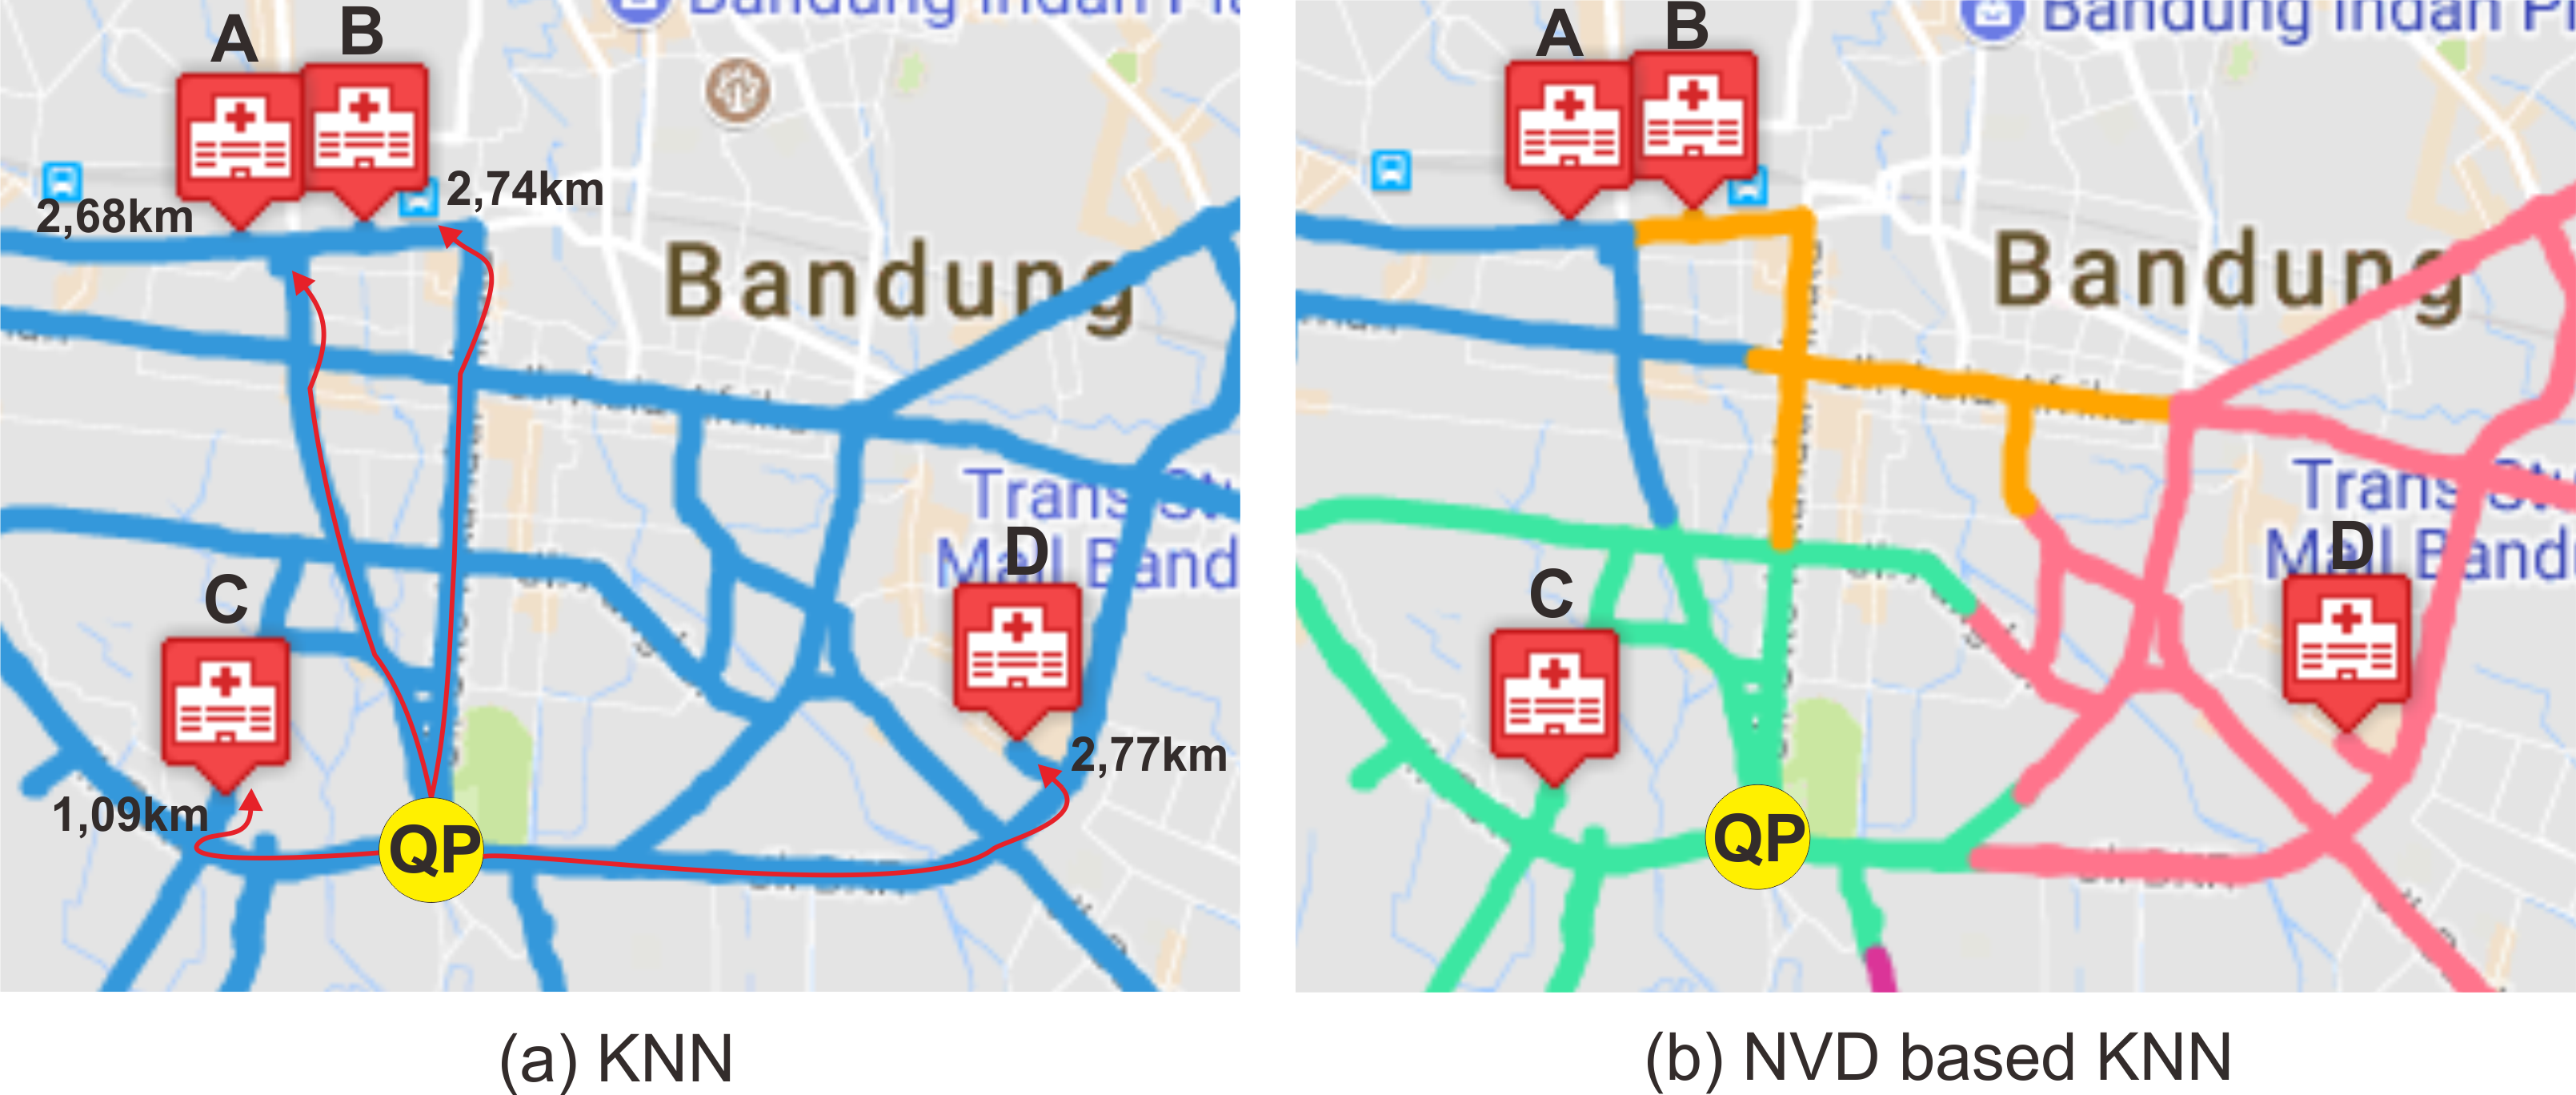
\includegraphics[scale=0.5]{illustration.png}
    \caption{Emergency services illustration in Bandung}
    \label{fig:illustration}
\end{figure}

In computer science, finding nearest emergency unit can be determine by using K-Nearest Neighbor (KNN) algorithm. Consider road network in Bandung shown in figure \ref{fig:illustration}(a), where emergency happens in Query Point (QP). KNN needs to determine each emergency unit distance to QP before comparing it and pick up the emergency unit with minimum distance. So in figure \ref{fig:illustration}(a), the nearest ambulance is C-ambulance. Notice that if there are emergency requests from many different location, then these process will repetead for each request. More requests means more processes KNN will takes.

Each emergency unit basically has a coverage area which specifies that its closer to the emergency unit than others. It can be done by using Network Voronoi Diagram (NVD) algorithm. NVD works as shown in figure \ref{fig:illustration}(b), where every road network's color represented each emergency unit's territories. So when emergency happens, NVD just needs to determine which emergency unit's territory emergency exist. In figure \ref{fig:illustration}(b) QP exist in C-ambulance with green territory which is the nearest ambulance.

This final project presents Network Voronoi Diagram based K-Nearest Neighbor development for 3 emergency services (ambulance, police, and fire brigade) in Bandung. In general, when an emergency occurs, user contact 112 to make a report. System will determine user coordinate location and select nearest emergency unit. System also support finding next nearest emergency units if nearest unit is on duty. The selected unit will be dispatch after receiving shortest path to the emergency location.

\pagebreak

\section{Problem Formulation}
Based on facts and problems mentioned in subsection motivation above, the main problems which will be discussed in this final project as follows :
\begin{enumerate}
	\item How to get k-nearest emergency unit to emergency location?
    \item How to find shortest path from selected units to emergency location?
\end{enumerate}

\section{Limitation of the Study}
To scope this final project to be more specific in accordance with the title and purpose, this final project limited to be discussed as follows :
\begin{enumerate}
    \item This final project only focused on emergency services in Bandung but only in west, south, east region.
    \item The road network used is the road segments that have functions as primary arterial roads, primary collector roads, secondary arterial road, and secondary collector road.
    \item Emergency units are divided into ambulance, police and fire brigade.
    \item Emergency unit selected is based on k-nearest from emergency location.
    \item Route determination from selected units to emergency location using shortest path ignoring road conditions.
\end{enumerate}


\section{Objective of the Study}
Based on the formulation of the above problems, this final project's objective are described as follows:
\begin{enumerate}
    \item To help operators determining k-nearest emergency unit from emergency location.
    \item To generate shortest path from emergency unit to emergency location so these unit can do first aid before fatal injury happens.
\end{enumerate}


\pagebreak
\iflogTA
\section{Systematic Writing}
The writing of the results in this report follows the description given in each successive chapter to facilitate discussion. From the subject matter can be divided into six chapters as described below :
\begin{enumerate}[label=Chapter I \hspace{5mm} : \hspace{2mm}, leftmargin=*, topsep=0pt, itemsep=-1ex, partopsep=1ex, parsep=1ex]
\item Introduction chapter contains an introduction that includes background, problem formulation, limitation of the study, objective of study, and systematic writing.
\end{enumerate}
\begin{enumerate}[label=Chapter II \hspace{3.5mm} : \hspace{2mm}, leftmargin=*, topsep=0pt, itemsep=-1ex, partopsep=1ex, parsep=1ex]
\item Review of Related Literature\\This chapter contains the theoretical foundations that support and directly relate to research to be conducted from books, research journals, internet, and other literary sources.
\end{enumerate}
\begin{enumerate}[label=Chapter III \hspace{2mm} : \hspace{2mm}, leftmargin=*, topsep=0pt, itemsep=-1ex, partopsep=1ex, parsep=1ex]
\item Method of Investigation\\This chapter contains a description of the steps of research conducted, but it is also a picture of author's mind frame in doing this final project from the beginning until it completed.
\end{enumerate}
\begin{enumerate}[label=Chapter IV \hspace{2mm} : \hspace{2mm}, leftmargin=*, topsep=0pt, itemsep=-1ex, partopsep=1ex, parsep=1ex]
\item Data Collection and Processing \\This chapter contains data collection process used in tis final project and contains process of data processing as an effort to create solutions for existing problems.
\end{enumerate}
\begin{enumerate}[label=Chapter V \hspace{3.5mm} : \hspace{2mm}, leftmargin=*, topsep=0pt, itemsep=-1ex, partopsep=1ex, parsep=1ex]
\item Result Analysis\\This chapter contains the analysis and data interpretation of the results in the previous section. The purpose of this section is to provide clear information about the results of this final project and able to provide solutions of the problems that arise.
\end{enumerate}
\begin{enumerate}[label=Chapter VI \hspace{2mm} : \hspace{2mm}, leftmargin=*, topsep=0pt, itemsep=-1ex, partopsep=1ex, parsep=1ex]
\item Conclusion\\This chapter contains the conclusions derived from the system design and analysis that have been done and the recommendations given for improvement.
\end{enumerate}
\else
\section{Plan Activity}
\begin{itemize}
	\item Study of literature
	
	At this stage, author tries to learn the concepts and theories about Network Voronoi Diagram also K-Nearest Neighbor from existing literature in books or international papers.
	\item Collecting Data

At this stage, author collecting necessary data as dataset by searching for information in advance on the internet and confirm it to speaker who are more competent.
\pagebreak
	\item Design and Implementation System

At this stage, author designing and implementation Network Voronoi Diagram KNN for building the system from problems.
	\item Testing and Analysis Results

In this stage, author do the test such  black box testing and white box testing. Author also gives the opportunity for some people to do the testing for strengthen the analysis results.
	\item Preparation of final report

At this stage, author preparing written report based on research conducted documentation and attach the conclusions and recommendations of the research results.
\end{itemize}

\fi
%
\chapter{Literature Review}
This final project discusses the design model to determining k-nearest emergency unit from emergency location. To establish the groundwork, this chapter will discuss theories and facts related.

\section{Emergency}
Emergency is an abnormal event that have negative impact. It can threaten and disrupt a person's life. An emergency can be presented in many forms; from everyday incidents like traffic accident or assault, to major incidents like wildfire, earthquake, or large-scale terrorist attacks. Emergency occurs suddenly with unexpected place and time \cite{hauke2011}.

\subsection{Emergency Services}

Emergency services ensure public safety by addressing emergency location and doing first aid. Basically there are three main emergency service functions which are law enforcement, emergency medical services, and fire service. These three function works as one and managed by emergency center. 

Emergency services vary widely in their use of technology. In some country, emergency services are reached by calling desired service by calling 7-digit telephone number, and then contacting the agency directly. In other areas, technology allows callers to use the single telephone number for every service they want.


\begin{figure}[H]
    \centering
    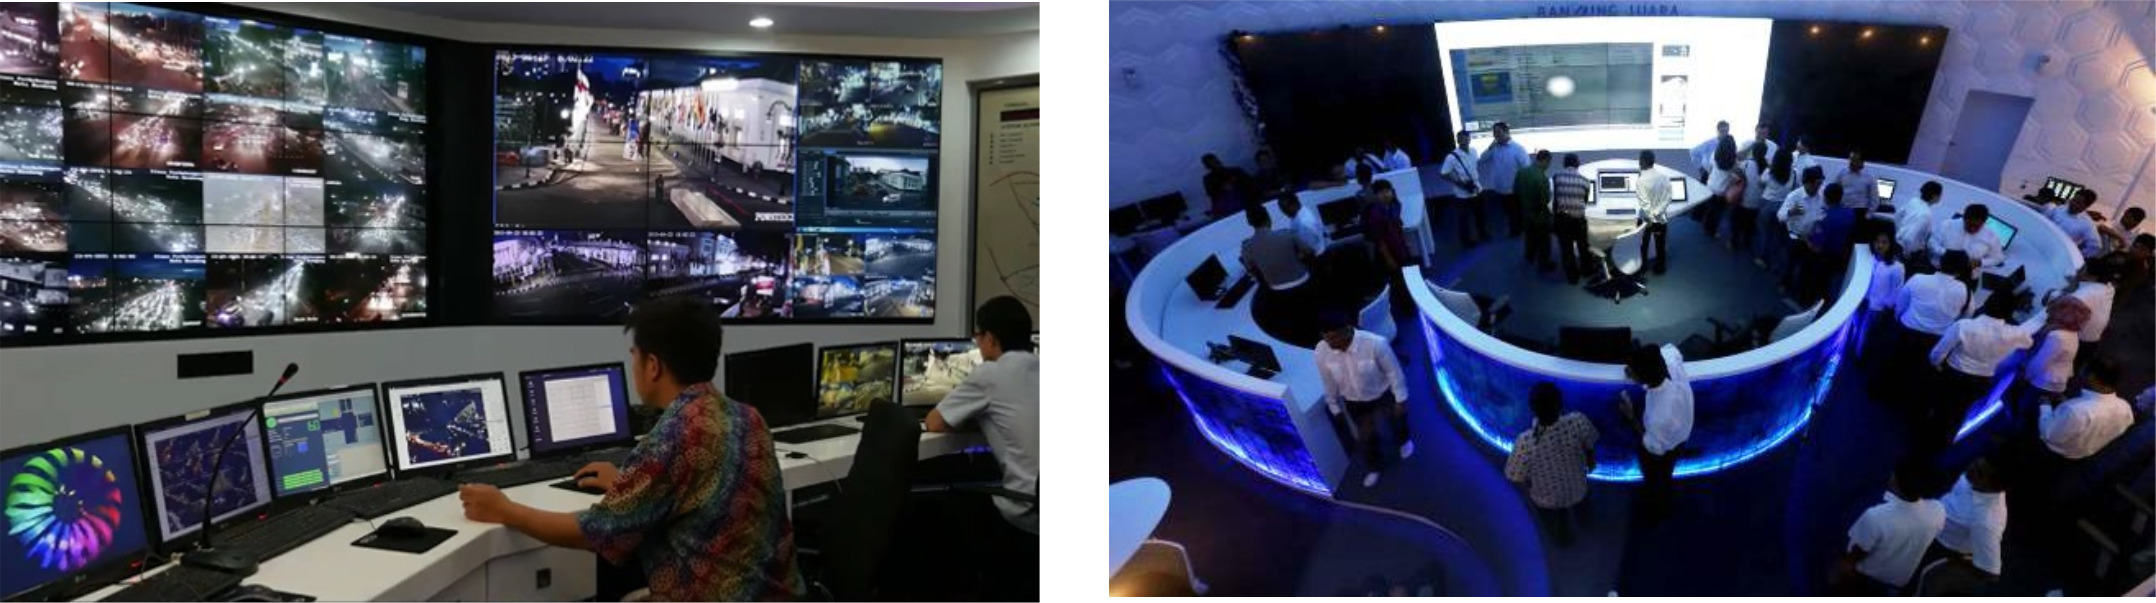
\includegraphics[scale=0.7]{emergency_center.png}
    \caption{Emergency Service Center in Bandung}
    \label{fig:emergency-units}
\end{figure}


\pagebreak
\subsection{Emergency Units}
Emergency unit is any unit that has to respond to an emergency in a life-threatening situation. In some major countries, the emergency unit consists of ambulance, police, and fire brigade. These units dispatched from a centre that takes calls from an emergency request. 

Many emergency units are likely to be fitted with audible and visual warning devices, which are designed to facilitate their movement through traffic to reach their destination, and to provide some protection on the scene. Traditionally, these units have relied on experience, practiced skills, good equipment, and teamwork for effective and successful emergency response.

\begin{figure}[H]
    \centering
    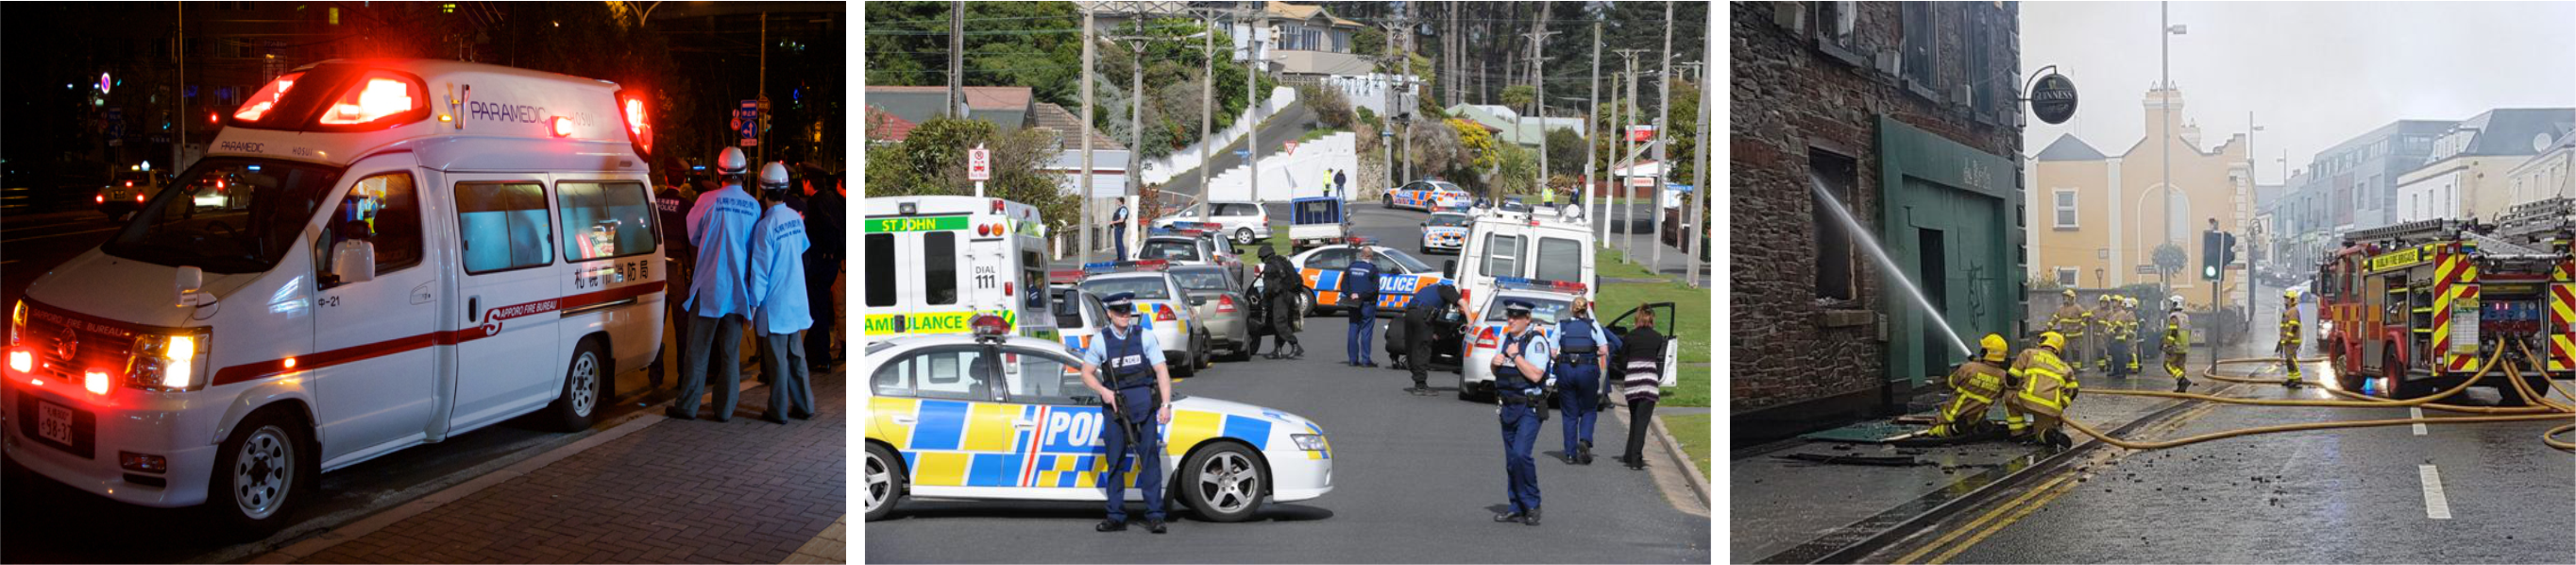
\includegraphics[scale=0.6]{emergency-units.png}
    \caption{Emergency Units consist of ambulance, police, and fire brigade}
    \label{fig:emergency-units}
\end{figure}

\section{Geographic Information System}
A GIS is required to monitor environmental conditions for various applications including policy making. This involves the use of data. A GIS will, in general, have a means of inputting data into a database, editing the data, displaying information stored in the database, and performing certain calculations including sorting of the data in the database. The nature of the data stored and the analytical and modeling capacity of a GIS will determine the solution to particular problems related to floods or land use planning or other potential needs \cite{ondieki1997}.

The role of a GIS is to enable the capture, storage, and manipulation of data in a structured form, therefore allowing the use of analytical techniques on the spatial dimensions of problems. With a GIS, analysis and depiction of spatially referenced information as well as dissemination of results of analysis using thematic maps is possible. Environmental science and other disciplines have generated enormous amounts of data of many different types, and this is bound to increase in future \cite{raju1997}.

\pagebreak
\subsection{Spatial Data}

In various fields there is a need to manage geometric, geographic, or spatial data, which means data related to space.  While typical databases have developed to manage various numeric and character types of data, such databases require additional functionality to process spatial data types efficiently, and developers have often added geometry or feature data types \cite{ooi1993}.

Spatial database is data that has, as a property, some connection with coordinates in a 2-dimensional, 3-dimensional space or even a higher dimensional space. Spatial data are large in quantity and are complex in structures and relationships. Spatial data properties shown as follows \cite{bonham-carter2014} :
\begin{enumerate}[leftmargin=*, topsep=5pt, itemsep=-1ex, partopsep=1ex, parsep=2ex]
\item Spatial Data Types: \\ It should support the point, line and surface types, since in daily practice people are familiar with the use of these objects.
\item Data Structures: \\ They should be simple. As opposed to the First Normal Form (1NN) relational model, for example, it is noticed that a nested model, though more powerful, is more difficult to both implement and use. Similarly, it is penalizing for the user to process two distinct data structures.
\item Spatial Operations: \\ They should apply to structures containing any type of spatial data.
\end{enumerate}

\begin{figure}[H]
    \centering
    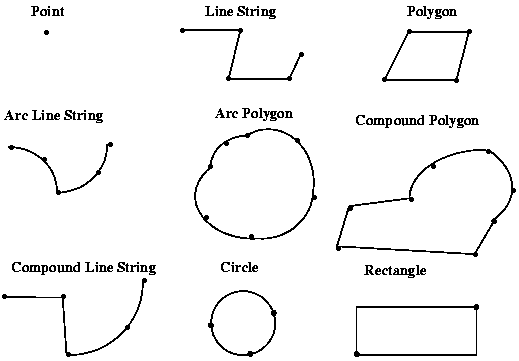
\includegraphics[scale=0.6]{spatial_data.png}
    \caption{Spatial Data Types}
    \label{fig:gis}
\end{figure}


\pagebreak
\subsection{Map Overlay}
The map overlay operation is a building block for various analysis operations in GIS. Its involves unions or intersection for two-map overlay. Map overlay works by executed as a sequence if binary map overlay operations. Map overlay implemented in either vector or raster system. In the vector case, often referred to as polygon overlay, the intersection of two or more data layers produces new features (polygons). Attributes (symbolized as colors in the illustration) of intersecting polygons are combined. The raster implementation (known as grid overlay) combines attributes within grid cells that align exactly. Misaligned grids must be resampled to common formats \cite{jampani2004}.

\begin{figure}[H]
    \centering
    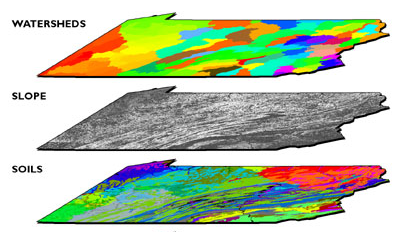
\includegraphics[scale=0.8]{map_overlay.png}
    \caption{map overlay illustration}
    \label{fig:gis}
\end{figure}


\section{Optimization Problems}
Optimization is the search for the values of variables that are considered optimal, effective, and efficient to achieve the desired goals. The optimization problem varies according to the conditions under which the system works. One of the most frequent optimization problems especially in the field of transportation is the search for the shortest path \cite{hannawati2002}.

Optimization in the shortest path can be based on the nearest distance to a facility or based on the fastest time to achieve it. This settlement process should still take into account the conditions that arise in it for a journey from the origin to the destination point such as traffic jam. The result of solving the shortest route problem can be called an optimal route. The optimal route is a route that has minimum travel time and distance.

\subsection{Solution of Optimization Problems}
To solving the problem of finding the shortest path can be done by using two methods, namely conventional method and heuristic method. Conventional methods are applied with ordinary mathematical calculations, while heuristic methods are applied with artificial intelligence calculations \cite{mutakhiroh2007}.
\pagebreak
\begin{enumerate}
\item The conventional method is a method that uses ordinary mathematical calculations. There are several conventional methods commonly used to perform the shortest path search, including: djikstra algorithm, Floyd-Warshall algorithm, and Bellman-Ford algorithm.

\item The heuristic method is a sub-field of artificial intelligence used for search and optimization. There are several algorithms on heuristic methods commonly used in optimization problems, including genetic algorithms, ant algorithms, fuzzy logic, neural networks, taboo search, simulated annealing, and others.
\end{enumerate}

\subsection{Solution of Shortest Path Problems}
The shortest path is a travel routing network in which a road steer wants to determine the shortest path between two cities, based on some available alternative paths, where the destination point is only one. The case can be illustrated as follows :

\begin{figure}[H]
    \centering
    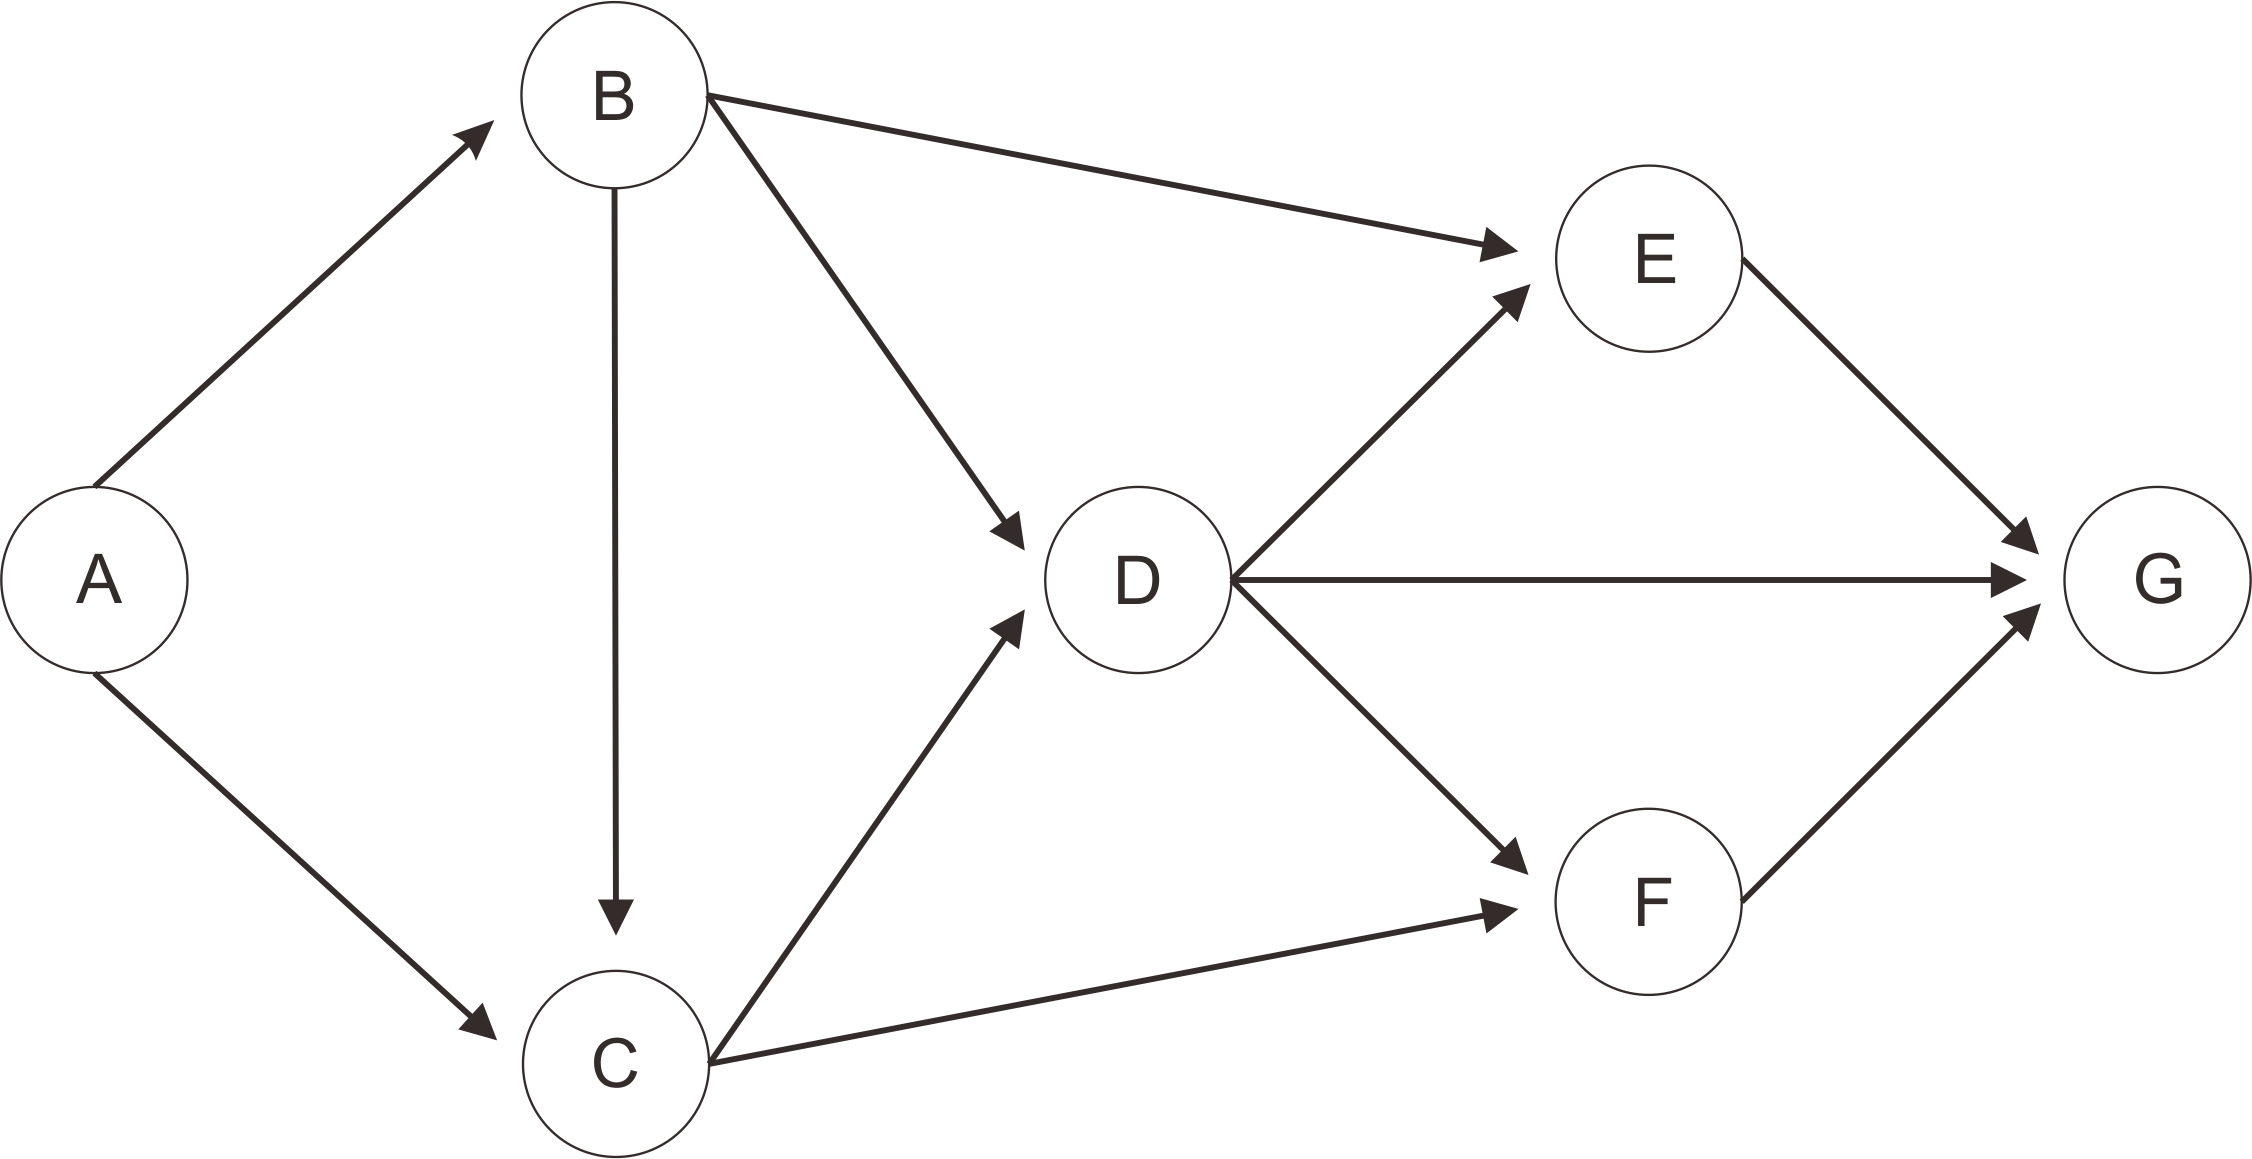
\includegraphics[scale=0.5]{graph-ABCDEFG.png}
    \caption{Graph ABCDEFG}
    \label{fig:graph-ABCDEFG}
\end{figure}

In \ref{fig:graph-ABCDEFG}, consider vertex A is the starting point and vertex G is the endpoint. To travel to vertex G there are many possible path which are :

\begin{enumerate}[leftmargin=*, topsep=5pt, itemsep=-1ex, partopsep=1ex, parsep=2ex]
\item $A \to B \to C \to D \to E \to G$ \hspace{10mm} 7. \hspace{0.5mm} $A \to B \to D \to G$
\item $A \to B \to C \to D \to F \to G$ \hspace{10mm} 8. \hspace{0.5mm} $A \to B \to E \to G$
\item $A \to B \to C \to D \to G$ \hspace{20mm} 9. \hspace{0.5mm} $A \to C \to D \to E \to G$
\item $A \to B \to C \to F \to G$ \hspace{20mm} 10. $A \to C \to D \to F \to G$
\item $A \to B \to D \to E \to G$ \hspace{20mm} 11. $A \to C \to D \to G$
\item $A \to B \to D \to F \to G$ \hspace{20mm} 12. $A \to C \to F \to G$
\end{enumerate}

Based on the above data, the shortest path can be calculated by finding the distance between the paths. If the distance between paths is not yet known, the distance can be calculated based on the coordinates of adjacent vertex.

\section{Road Network System}
Road network system is a unity of road network consisting of primary road network system and secondary road network system interwoven in hierarchy relationship. The road network system is structured with reference to the spatial plan of the region and with respect to interconnection and/or interconnection within urban areas, and rural areas \cite{zhang2005} \cite{weiping1989}.

\begin{figure}[H]
    \centering
    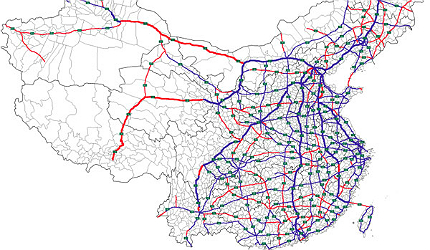
\includegraphics[scale=0.7]{road-network.jpg}
    \caption{Road Network System}
    \label{fig:Road Network System}
\end{figure}

\subsection{Road Classification}
The road is a land transport infrastructure covering all parts of the road, including auxiliary buildings and equipment intended for traffic, located on the soil surface, above ground level, below ground and / or water, and above water level, Lorries, and cable roads.

Road classification based on its function according to UU no. 38/2004 includes:
\begin{enumerate}[label=- , leftmargin=*, topsep=5pt, itemsep=-1ex, partopsep=1ex, parsep=2ex]
\item Arterial road is a public road that serves the main transport with long-distance travel features, high average speed, and the number of entrances are limited efficiently.
\item Road collector is a public road that serves to serve the collector or the spacer with medium distance features, moderate average speed, and the number of entrances is limited.
\item Local roads are public roads that serve local transport with features of short distance travel, low average speed, and unlimited number of entrances.
\item The road environment is a public road that serves the transportation of the environment with the characteristics of travel at close range, and with low average speed.
\end{enumerate}

\pagebreak

\section{K-Nearest Neighbor}
K-Nearest Neighbor (KNN) is one of classification algorithm that classifies by proximity of data with others data. In the KNN algorithm of q-dimensional data, the distance from the data to others data can be calculated. Distance values are used as proximity values or similarities between data testing and datasets. The K value of the KNN algorithm is the closest amount of data from the data testing. If K = 1, then the class of data testing is the class of the nearest neighbor. If k = 3, three closest neighbors will be taken from the dataset \cite{prasetyo2012}.

KNN is one of the most widely used algorithms in machine learning. KNN is a learning method based on the case and no learning phase is required (training). The model developed in the KNN algorithm is a training sample relating to the distance function and the choice of class function based on the nearest neighbor class. The functioning of the method depends on the choice of some number of parameters such as the K parameter representing the number of neighbors selected to assign the new data class and the distance calculation method used \cite{medjahed2013}.

\subsection{KNN Classification}
Let G is a set of a data in dataset which has class. KNN compute distance from Q to each data in dataset. Then KNN sort data with minimum distance before determine class for Q. If k=1, Q's class of data testing is the class of $g_{1}$. If k=3, Q gets three closest neighbors which is $g_{1}$, $g_{2}$, and $g_{3}$.

\begin{figure}[H]
    \centering
    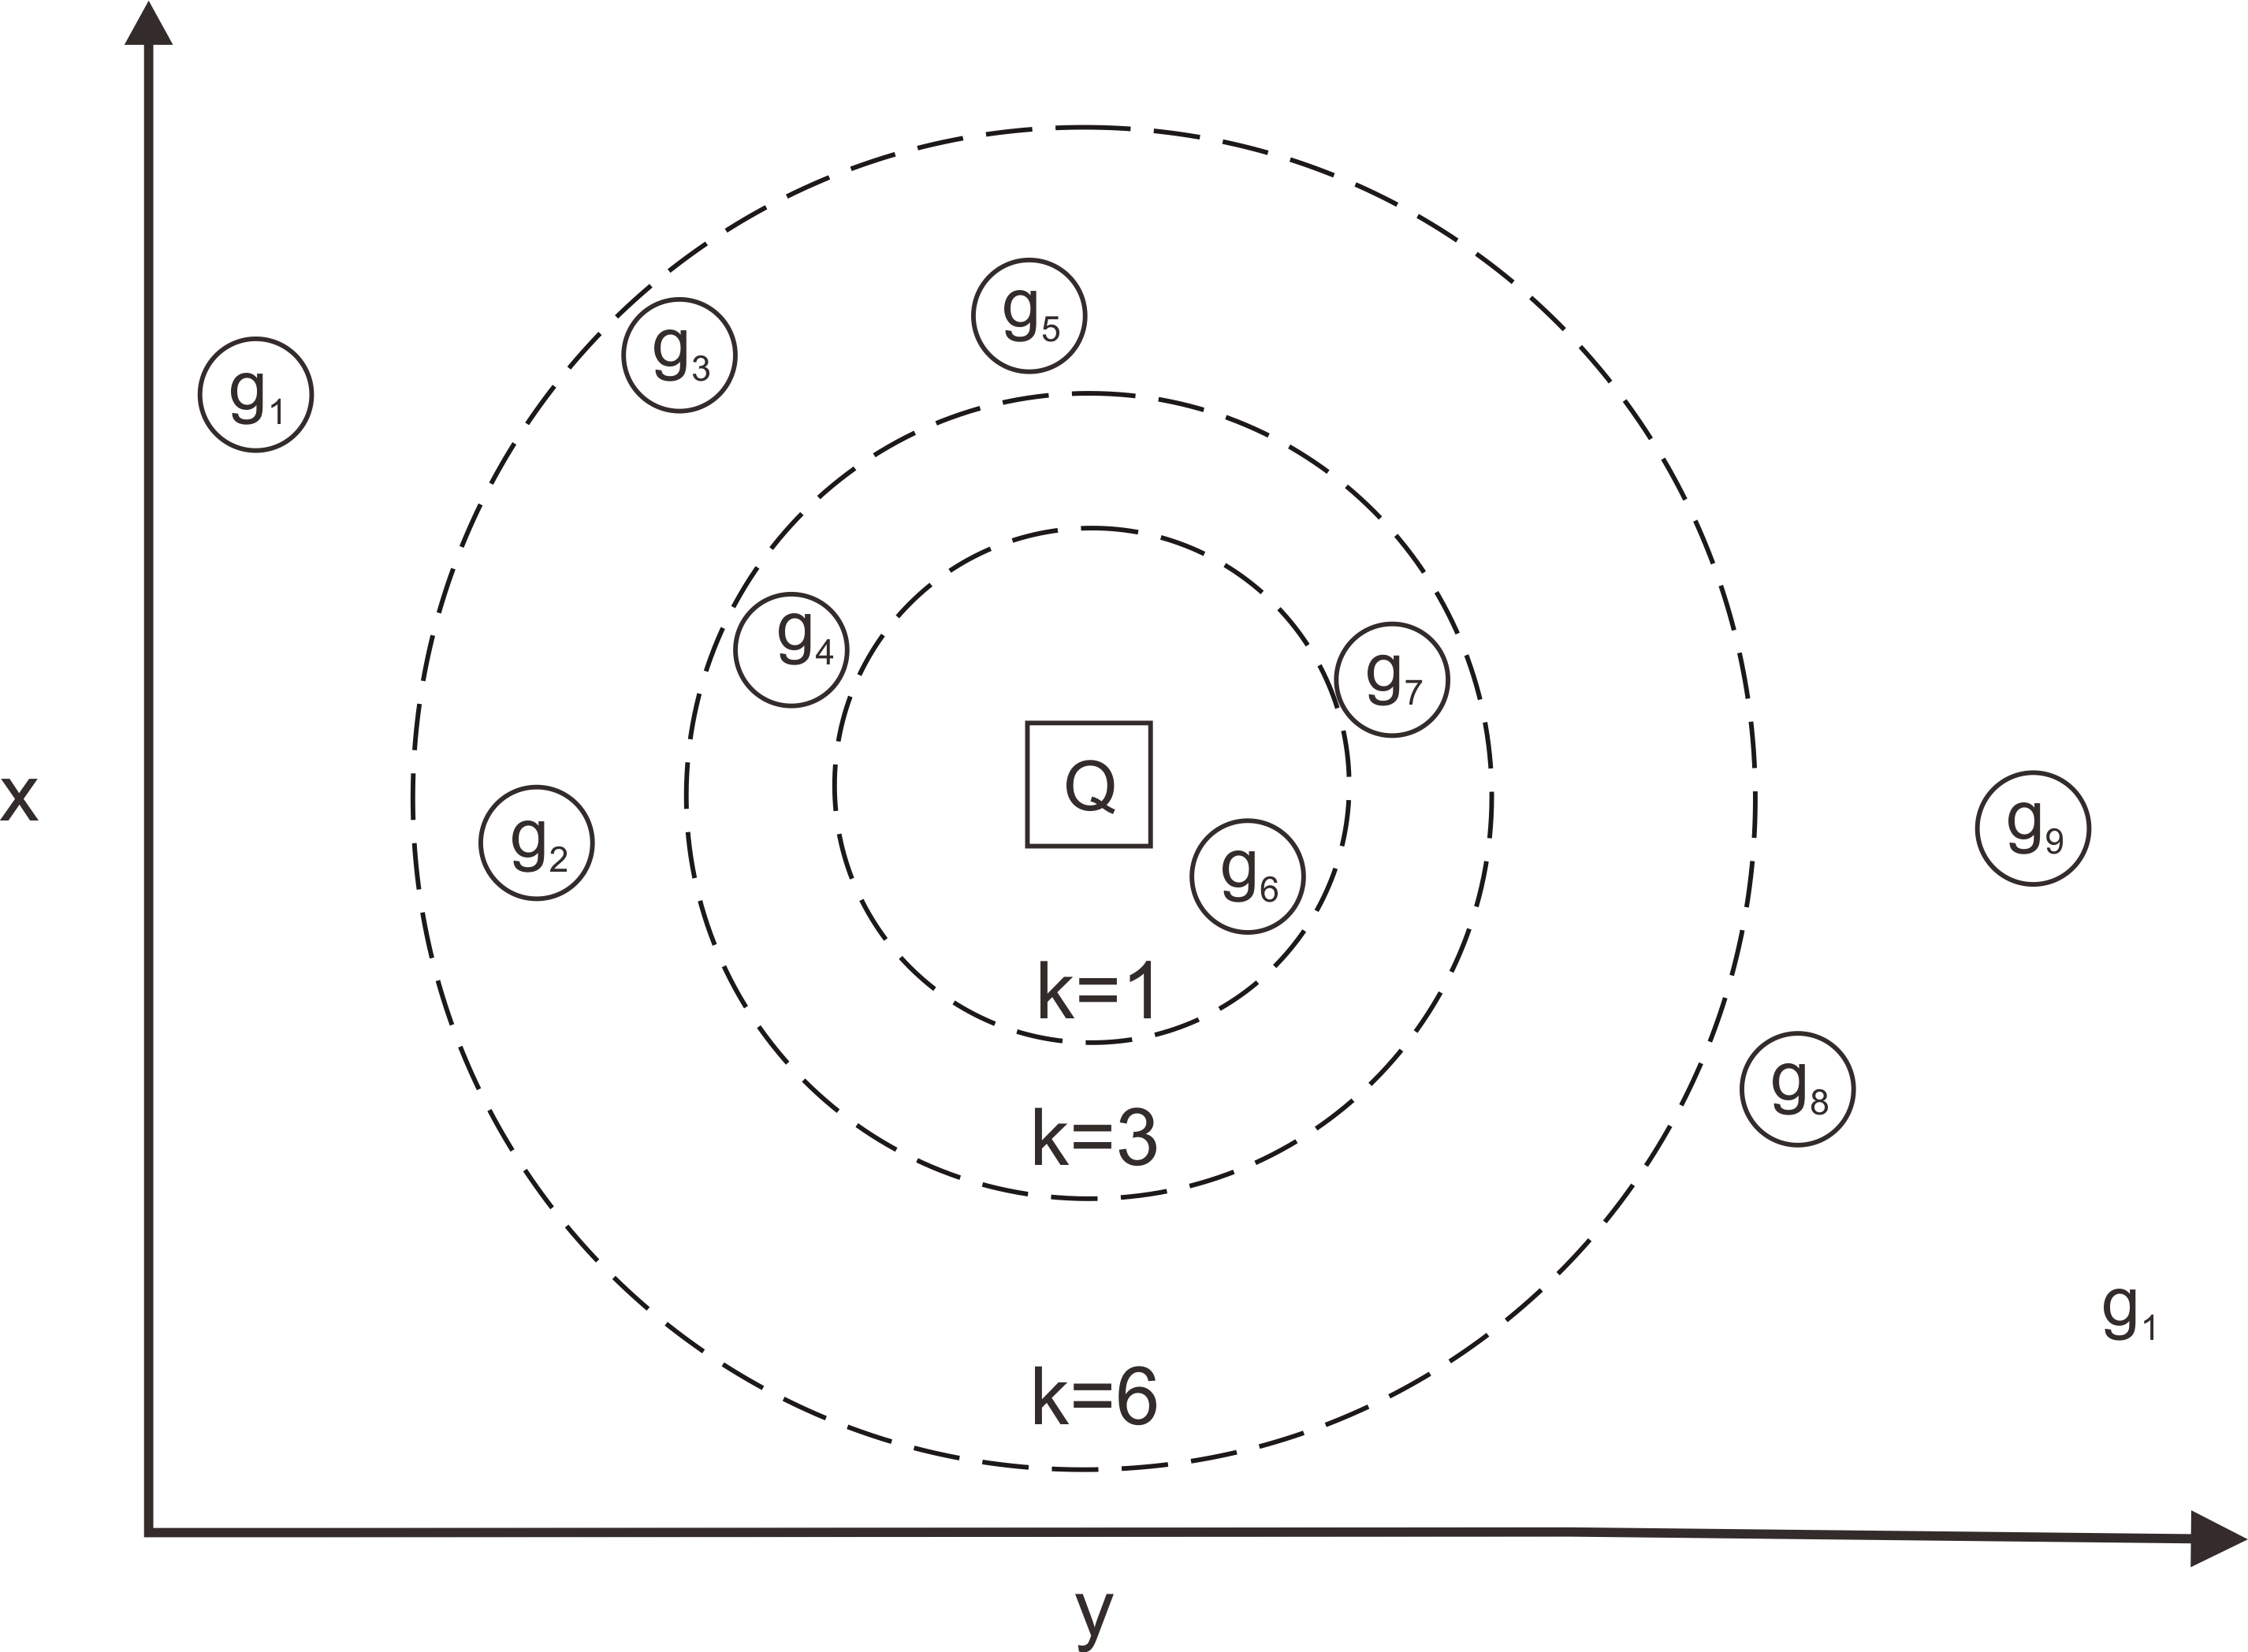
\includegraphics[scale=0.4]{knn.png}
    \caption{K-Nearest Neighbor}
    \label{fig:KNN}
\end{figure}



\subsection{Advantages and Disadvantages from KNN}
KNN algorithm has several advantages including KNN algorithm is a simple classification algorithm, the resilience of dataset interference, and effectiveness in the dataset adequate. However, the KNN algorithm also has disadvantages as follows \cite{zhang2013} :

\begin{enumerate}[label=- , leftmargin=*, topsep=5pt, itemsep=-1ex, partopsep=1ex, parsep=2ex]
\item KNN algorithm has a high computational cost. To determine the nearest k-neighbor of a data testing, all similarities between the data testing and the dataset must be calculated.
\item KNN algorithm has a dependency on the dataset. The resulting classification is only based on the sample dataset and does not use any additional data. This makes the KNN algorithm highly dependent on the dataset.
\item KNN algorithm also has weaknesses in terms of low accuracy in multidimensional data sets, K parameters, and distance calculation methods.
\end{enumerate}


\section{Voronoi Diagram}
The Voronoi Diagram has been applied to many location problems \cite{okabe2000}. The Voronoi diagram is data structure extensively in the domain of computatuional geometry. Originally, it characetrizes regions of proximity for a set of $k$ sites in the plane where distance poinrs is defined by their Euclidean distance. Optimal algortihms exist to compute the Voronoi diagram in $0(k log k)$ time, and the Voronoi diagram can be represented in $0(k)$ space \cite{erwig2000}.

\begin{figure}[H]
    \centering
    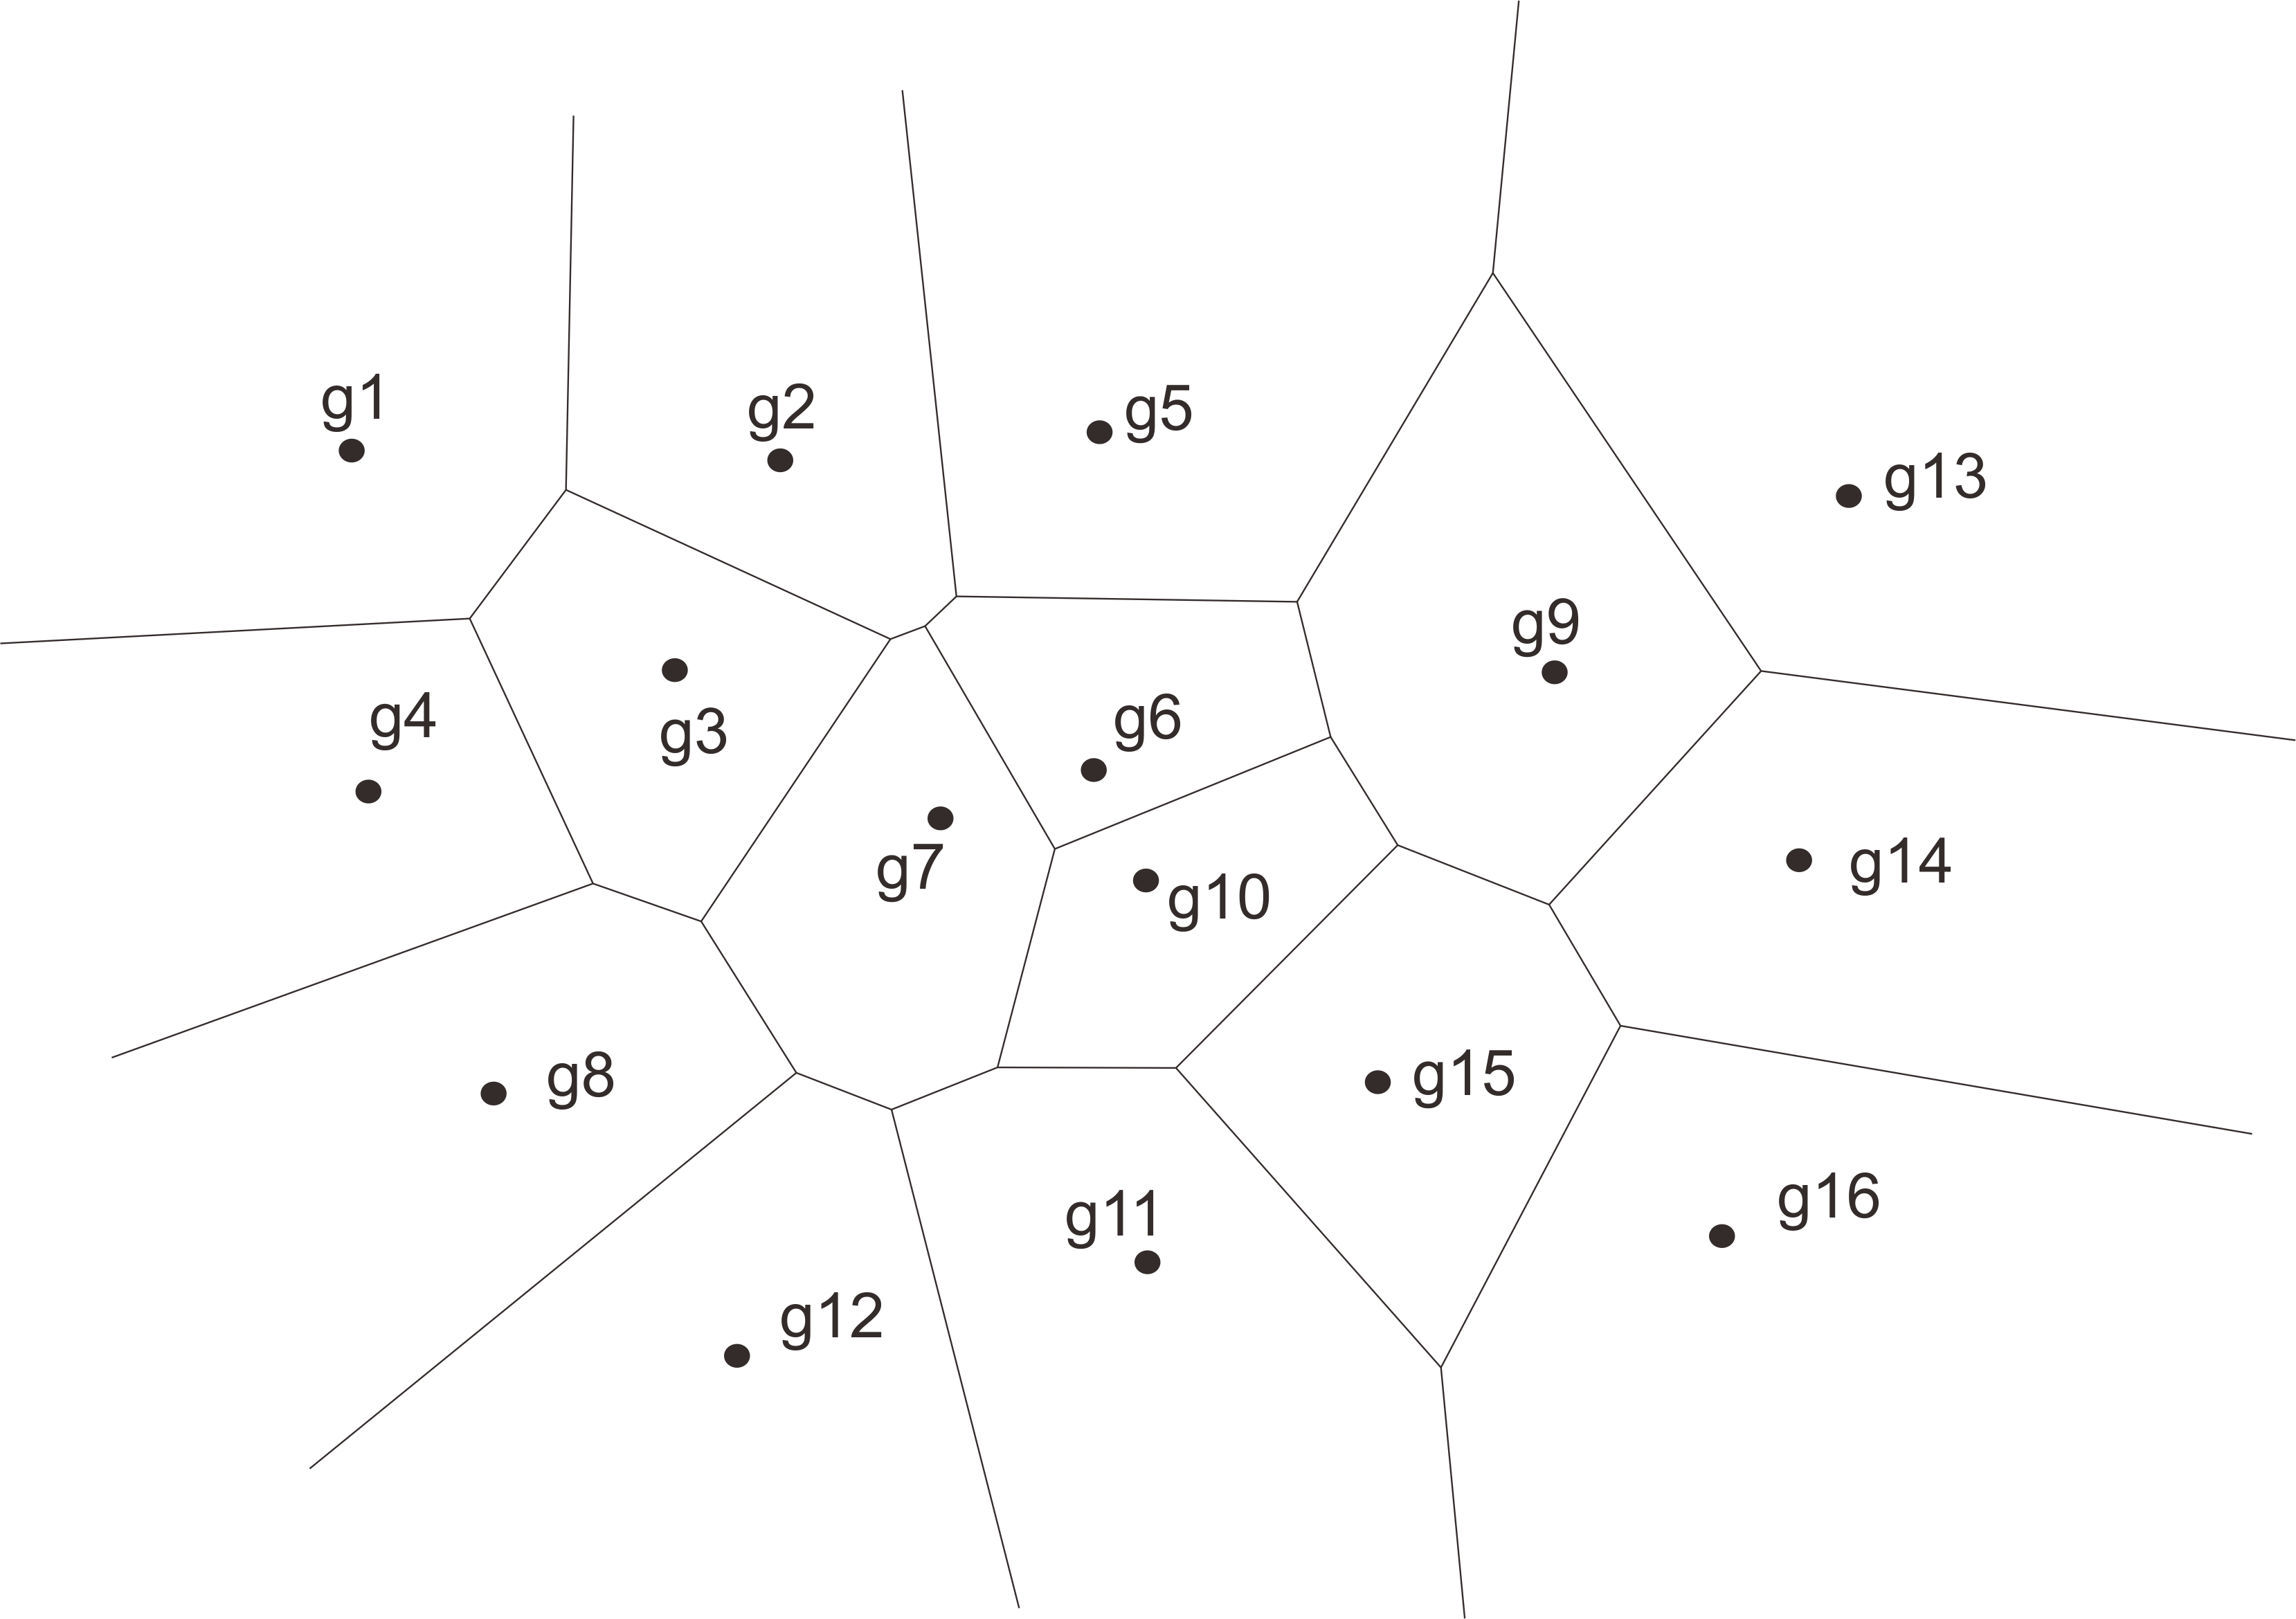
\includegraphics[scale=0.4]{voronoi-diagram.png}
    \caption{Voronoi Diagram}
    \label{fig:my_label}
\end{figure}

For example there is a set point generator on Euclidean field (in general, the generator can be any type of spatial objects). Consider all locations in the area has been associate for their closest generator. Set the location assigned to each generator forming region called Voronoi cell. This Voronoi Cell basically based of it generator. More specifically, Voronoi polygon formed by dividing border point which is the middle point betweens the generator with it adjacent generators. Set of Voronoi polygon formed is called a Voronoi diagram.

There are 4 review from basic geometric properties of the Voronoi diagrams as follows \cite{kolah2004} :
\begin{enumerate}[label=- , leftmargin=*, topsep=5pt, itemsep=-1ex, partopsep=1ex, parsep=2ex]
	\item Property 1: The Voronoi diagram of a point set $G$, $VD(G)$, is unique.
	\item Property 2: The nearest generator point of $g_{i}$ (e.g., $g_{j}$) is among the generator points whose Voronoi polygons share similar Voronoi edges with V P(pi).
	\item Property 3: Let $n$ and $n_{e}$ be the number of generator points and Voronoi edges, respectively, then $n_{e} \leq 3n - 6$.
	\item Property 4: From property 3, and the fact that every Voronoi edge is shared by exactly two Voronoi polygons, notice that the average number of Voronoi edges per Voronoi polygon is at most 6, i.e., $2(3n-6)/n = 6/12n \leq 6$. This means that on average, each generator has 6 adjacent generators.
\end{enumerate}



\section{Network Voronoi Diagram}
Voronoi diagram in the plane is sometimes inadequate for the location problem \cite{takehiro2005}. The reason is that the distances can not be measured by the Euclidean distances in some problems. So there’s a network and defined by nodes and arcs which is the partition of the two.

\begin{figure}[H]
    \centering
    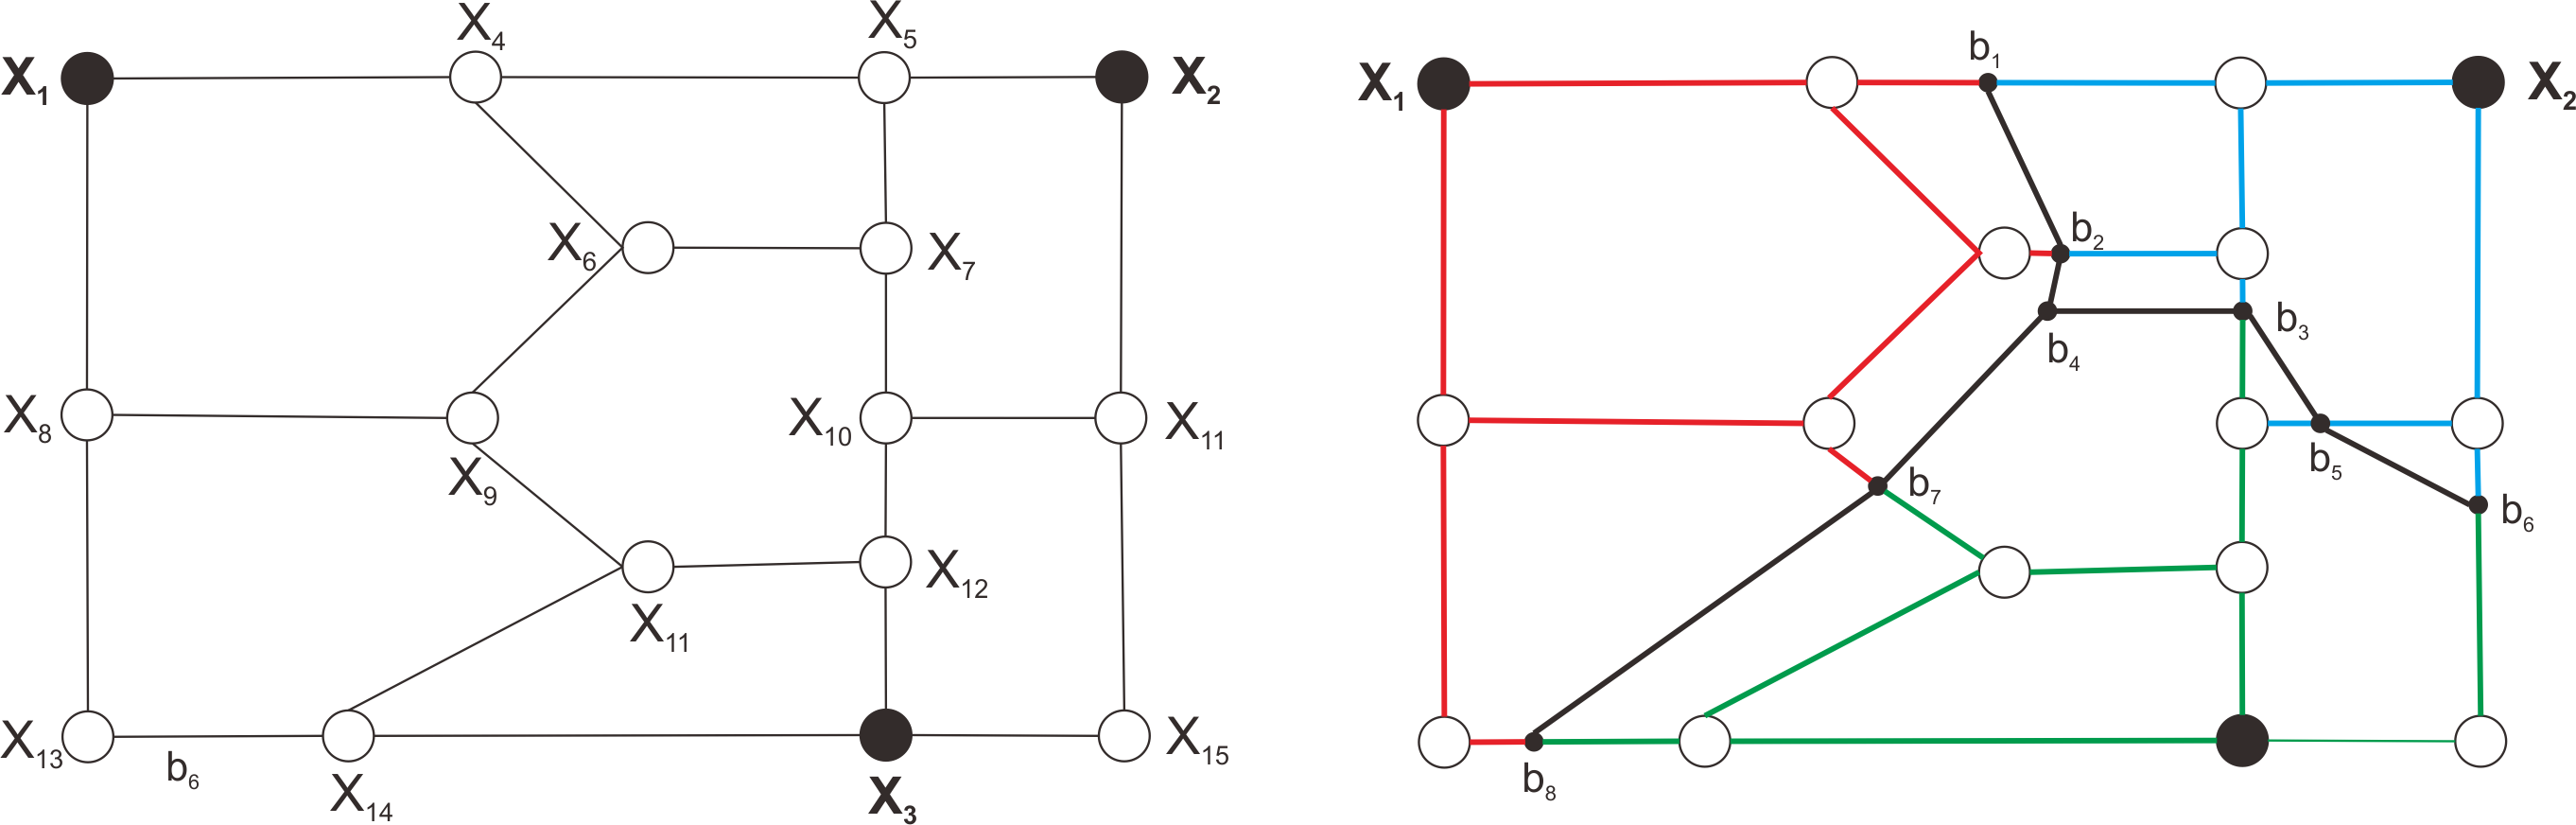
\includegraphics[scale=0.6]{network-voronoi-diagram.png}
    \caption{Network Voronoi Diagram}
    \label{fig:my_label}
\end{figure}    
    
\pagebreak
Network Voronoi diagram is based on Djikstra's algorithm calculates in  a connected network \cite{erwig2000}. NVD is defined by consider a network $N(V, E)$ and a set of vertices $V = {x_{1}, x_{n}, x_{n+1} ..., x_{o}} \subseteq V$, where the first $n$ elements (ie., $G = {g_{1}, ..., g_{n}}$) are the generators (e.g., points of interest in road network). Each edge in $N(V, E)$ has positive length. All vertices that are closer to $g_{i}$ represent $g_{i}$ dominance over its adjacent generator. The set $b(g_{i}, g{j})$, called border points between $g_{i}$ and $g_{j}$, specifies all points in all edge that are equally distance from $g_{i}$ and $g_{j}$.

The algorithm for computing the Network Voronoi Diagram is shown in the following pseudocode.

\begin{algorithm}
\caption{Network Voronoi Diagram Algorithm}
\begin{algorithmic}[1]
\Procedure{constructNVD}{}
\ForEach {$v \in S$}:
	\If{$v \in G$}
		\State $V(v)\gets g$
		\State $d(v)\gets 0$
		\State $insert(v)$
	\Else
		\State $V(v)\gets null$
		\State $d(v)\gets \infty$
	\EndIf
\EndFor

\While{$Queue\not=empty$}
	\State $v_{min}\gets extractmin()$
	\State mark  $v$
	\ForEach{$neighbor(v, w)$ with $w$ not marked}
		\State $\Delta\gets d(v_{min}) + l(v, w)$
		\If{$d(w) = \infty$}
			\State $d(w)\gets \Delta$
			\State $V(w)\gets V(v_{min})$
			\State $insert(w)$
		\Else
			\State $V(w)\gets V(v)$
			\State $decreaseKey(w, \delta)$
		\EndIf
	\EndFor
\EndWhile
\EndProcedure
\end{algorithmic}
\end{algorithm}

\pagebreak
\section{K-Nearest Neighbor in Network Voronoi Diagram} 

The k-nearest neighbor Voronoi diagram has also important uses in computation geometry and in location problems. Given the set of the generator g in a space S and query point QP. Let d(g) denotes distance g to QP. For each g, d(g) will be computed and store it at queue. After that, queue being sorted by minimum distance. So by looking into queue order k-nearest generator will be found.
\begin{figure}[H]
    \centering
    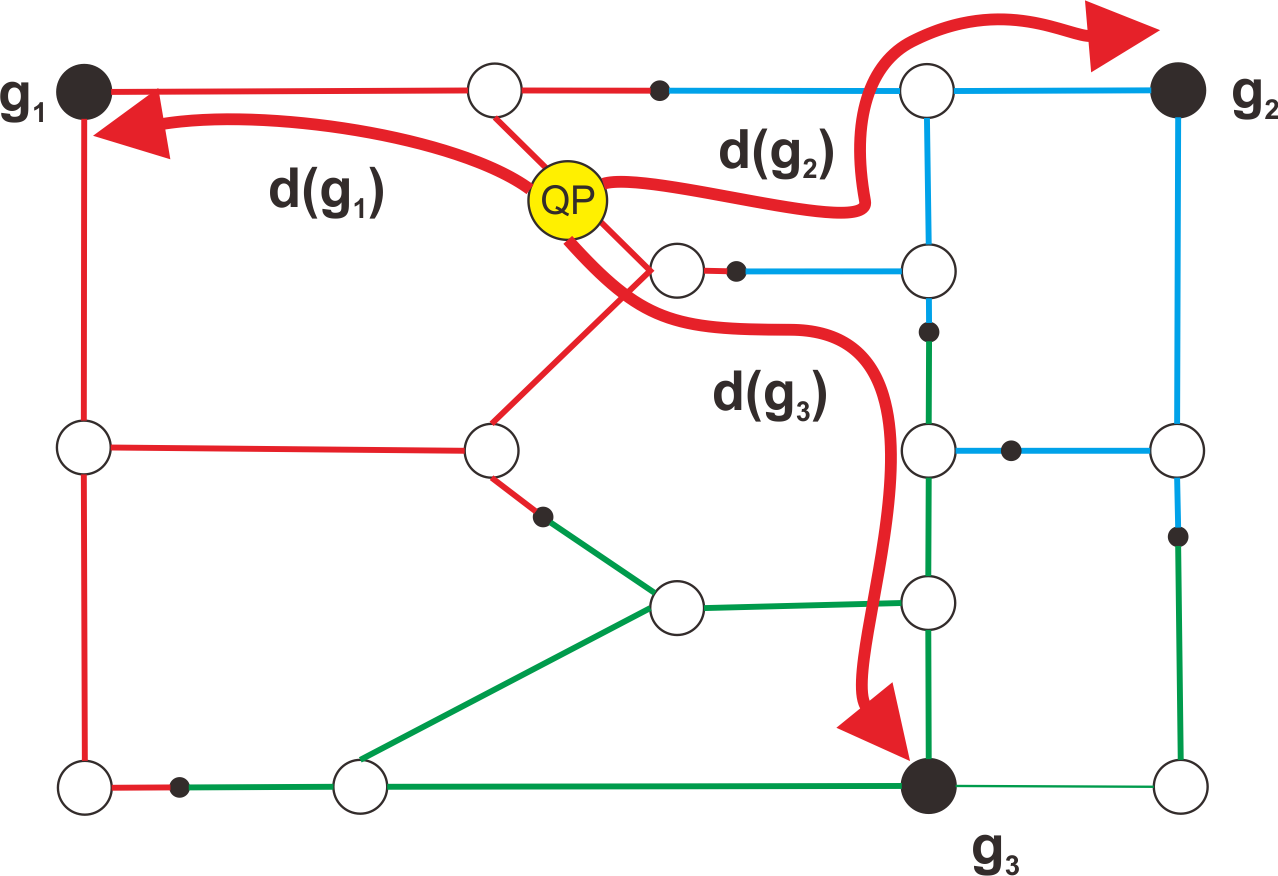
\includegraphics[scale=0.8]{knn_basic.png}
    \caption{KNN algorithm in road network}
    \label{fig:my_label}
\end{figure} 

The algorithm for computing the K-Nearest Neighbor in Network Voronoi Diagram is shown in the following pseudocode.

\begin{algorithm}
\caption{Basic KNN Algorithm in NVD}
\begin{algorithmic}[1]
\Function{KNN($QP$, $k$)}{}
\ForEach {$g \in S$}:
	\State $d(g) \gets count_distance(g, QO)$
	\State $insert(g)$
\EndFor
\State $sort Queue by minimum d$
\Return $Queue[k]$
\EndFunction
\end{algorithmic}
\end{algorithm}

%
\chapter{Method of Investigation}
A study requires a methodology to minimize errors in decision making. This chapter describes systematically the overview of the methodology used in this study. The steps performed are shown in figure \ref{fig:research_methodology_flow_diagram_1} and \ref{fig:research_methodology_flow_diagram_2} below :

\begin{figure}[H]
    \centering
    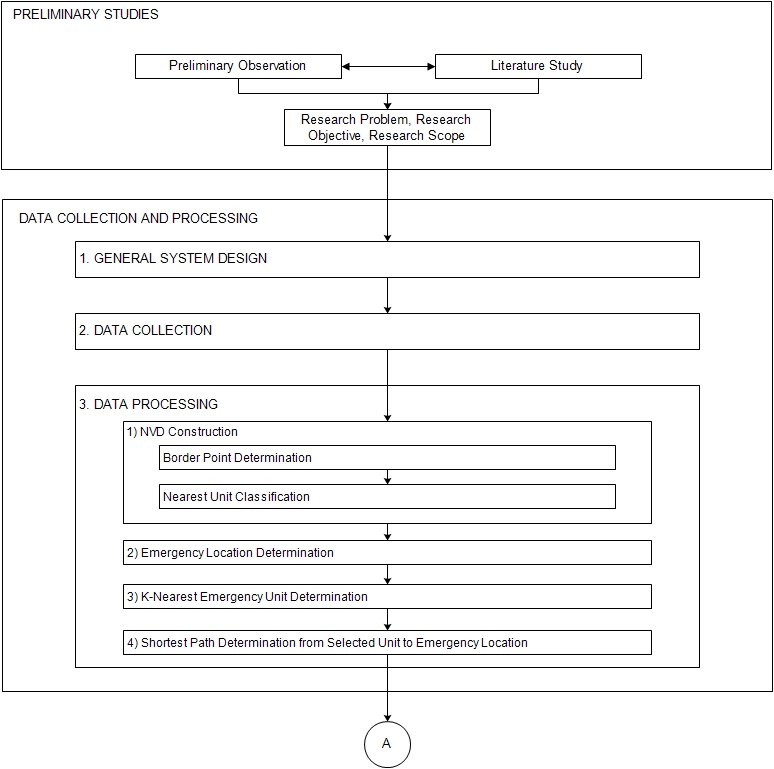
\includegraphics[scale=0.65]{flow_diagram_metodologi_penelitian_1.jpg}
    \caption{Methodology Flow Diagram (1)}
    \label{fig:research_methodology_flow_diagram_1}
\end{figure}

\begin{figure}[H]
    \centering
    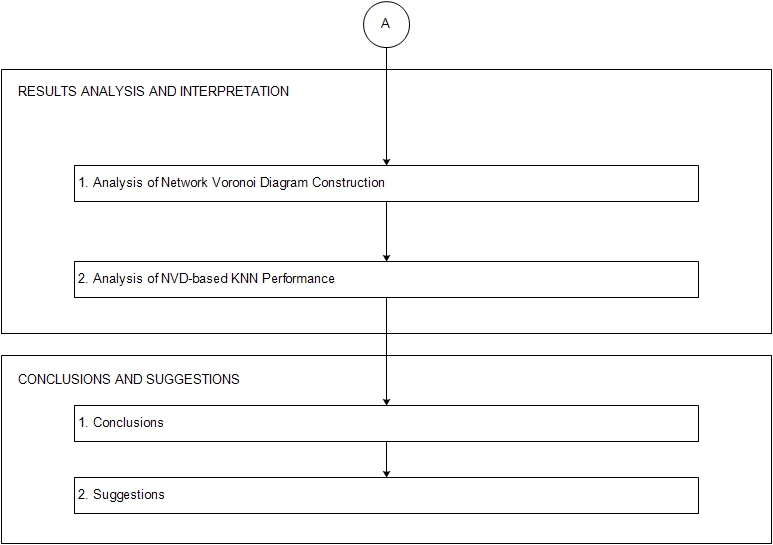
\includegraphics[scale=0.65]{flow_diagram_metodologi_penelitian_2.jpg}
    \caption{Methodology Flow Diagram (2)}
    \label{fig:research_methodology_flow_diagram_2}
\end{figure}

\section{Preliminary Studies}
Initial observations are made by observation to the field directly. Field observation process provides an overview of the problems that exist, then this problem put together into the formulation of the problem. Formulation of problems that arise that is how to determine the nearest emergency unit from emergency location and compute route to it based on the shortest path.

This literature study was conducted to support the process for this study. Some of the literature used are the study of first aid emergency, the study of network voronoi diagram, the study of k-nearest neighbor, and analysis of the road network using geographic information system. Sources of literature comes from books, journals, previous study related, and also sources of information from the internet.
\pagebreak

\section{General System Design}
The purpose of system design in general is to provide a general overview of the system built and identify the components of the systems that will be designed in detail.

\subsection{System Description}
The system built on this research is the first aid emergency system by using Network Voronoi Diagram based K-Nearest Neigbor. In general, the system can be seen in figure \ref{fig:system_description} below. First, system accepts input user location where emergency happens. Then the system will process the input to determine nearest emergency units to emergency location that has been divide using Network Voronoi Diagram. If the selected unit is on duty, system will looking for next nearest emergency unit using K-Nearest Neighbor. After k-nearest emergency unit selected, system determines the shortest path from their location to emergency location. And the last, system sends data to the results of this process to each selected emergency unit so that they can immediately go to the emergency location to do first aid.

\begin{figure}[H]
    \centering
    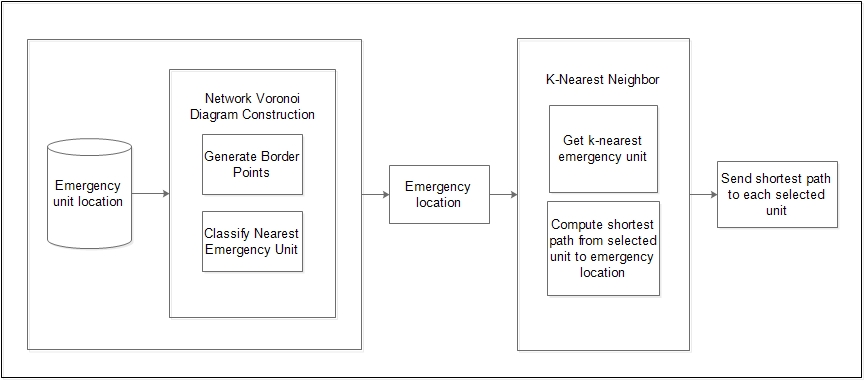
\includegraphics[scale=0.6]{system-desc.jpg}
    \caption{System Description}
    \label{fig:system_description}
\end{figure}
\pagebreak

\subsection{System Flowchart}

\begin{figure}[H]
    \centering
    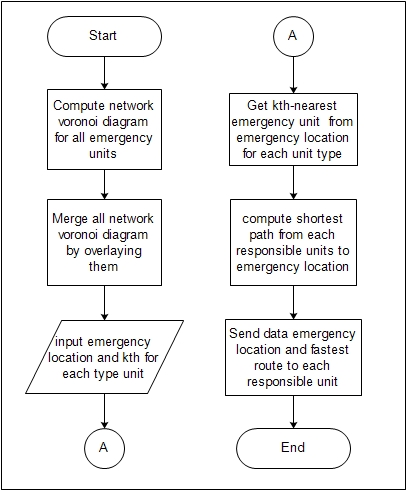
\includegraphics[scale=0.7]{system-flow.jpg}
    \caption{System Flowchart}
    \label{fig:system_flowchart}
\end{figure}


\begin{enumerate}[leftmargin=*, topsep=5pt, itemsep=-1ex, partopsep=1ex, parsep=2ex]
	\item System determining border points for all emergency units as a middle point between adjacent units.
    \item System construct network voronoi diagram to get each vertex perspective about its nearest emergency unit so it will make a territory for each unit in same unit type.
    \item System merge all network voronoi diagram (nvd for ambulance, nvd for police, and nvd for fire brigade), which has been constructed by overlaying all of them.
    \item System gets emergency location inputs where emergency occurs.
    \item System determining nearest unit to emergency location. If selected unit is on duty, system will looking into next nearest unit. Until system find it an appoint it as responsible unit.
    \item System compute shortest path from each responsible units to emergency location.
    \item System sends data emergency coordinates location and shortest path from each responsible units to the location.
\end{enumerate}
\pagebreak


\section{Data Collection and Processing}
Data collection and processing are used to get the final result of the nearest emergency units(police, ambulance, fire brigade) from emergency location (traffic accident) and compute route to it.

\subsection{Data Collection}
Data collection needed as support for determining nearest emergency unit from emergency location. The data collected are:

\begin{enumerate}[label=- , leftmargin=*, topsep=5pt, itemsep=-1ex, partopsep=1ex, parsep=2ex]
\item Bandung road network map\\
These map contains some public road network in Bandung City partially including south side, west side, east side, and center side. The public road network includes arteries and collector road type.
\item Coordinate location data of ambulance units\\
These coordinate location data of ambulance units are obtained from portal data Bandung.
\item Coordinate location data of police units\\
These coordinate location data of police units are obtained from Kepala Polisi Resor Bandung and portal data Bandung.
\item Coordinate location data of fire brigade units\\
The coordinate location data of police units are obtained from Dinas Pemadam Kebakaran Bandung and portal data Bandung.
\end{enumerate}

\subsection{Data Processing}
Data processing step serves to find responsible units and generate shortest path from them to emergency location. This step can be explained as follows:

\subsubsection{3.3.3.2.1 Process of Constructing NVD}
This step works by divide Bandung into coverage area for each emergency unit. The coverage area denotes that every location inside the coverage area will return its emergency unit as nearest emergency unit. NVD construction also looking for neighborhoods between adjacent emergency unit which used for searching next nearest emergency unit. NVD Construction consists of the process of determining border points and process of nearest unit classification.

\pagebreak

\subsubsection{Process of Determining Border Point}
\begin{enumerate}[label=Input\hspace{5mm} :\hspace{2mm}, leftmargin=*, topsep=0pt, itemsep=-1ex, partopsep=1ex, parsep=1ex]
\item road network, ambulance units coordinate point, police units coordinate point, fire brigade units coordinate point
\end{enumerate}
\begin{enumerate}[label=Output\hspace{2mm} :\hspace{2mm}, leftmargin=*, topsep=0pt, itemsep=-1ex, partopsep=1ex, parsep=1ex]
\item ambulance units border point, police border point, fire brigade border point
\end{enumerate}
Border point denotes middle distance from two adjacent emergency units. Border point will act as outer parts from a emergency unit's territory. To determining border points, system needs to read road network and also coordinate point of each emergency unit. After system reads the input, each emergency units will be selected as starting point and expand to other vertex which share same edge with them. Border point obtained when expanding process meets another emergency unit.

\begin{figure}[H]
    \centering
    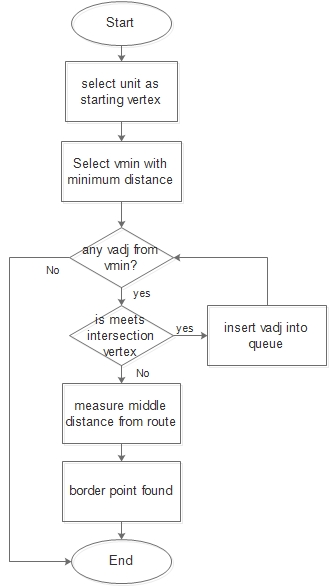
\includegraphics[scale=0.8]{flowchart_bp.jpg}
    \caption{Flowchart Border Point Determination}
    \label{fig:bp_pol}
\end{figure}

\pagebreak
\subsubsection{Process of Classifying nearest unit}
\begin{enumerate}[label=Input\hspace{5mm} :\hspace{2mm}, leftmargin=*, topsep=0pt, itemsep=-1ex, partopsep=1ex, parsep=1ex]
\item road network, ambulance units coordinate point, ambulance units border point, police units coordinate point, police units border point, fire brigade units coordinate point, fire brigade units border point
\end{enumerate}
\begin{enumerate}[label=Output\hspace{2mm} :\hspace{2mm}, leftmargin=*, topsep=0pt, itemsep=-1ex, partopsep=1ex, parsep=1ex]
\item ambulance units network voronoi diagram, police network voronoi diagram, fire brigade network voronoi diagram
\end{enumerate}
This step works by classifying nearest generator (1-NN) for each vertex in plane. Network voronoi diagram will shows territory of each unit in same type. To construct NVD, system needs to read road network and all vertex including generator, border points, or normal vertex. This process will be computed three times because there are three types of units (police, ambulance, fire brigade).

\begin{figure}[H]
    \centering
    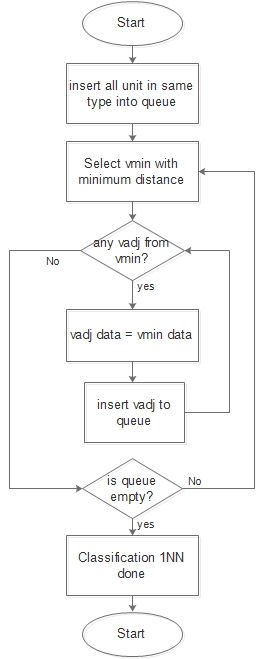
\includegraphics[scale=0.75]{flowchart_classify.jpg}
    \caption{Flowchart Nearest Unit Classification}
    \label{fig:bp_pol}
\end{figure}

\pagebreak
\subsubsection{3.3.3.2.2 Process of Determining Emergency Location}
\begin{enumerate}[label=Input\hspace{5mm} :\hspace{2mm}, leftmargin=*, topsep=0pt, itemsep=-1ex, parsep=1ex]
\item emergency coordinate location
\end{enumerate}
\begin{enumerate}[label=Output\hspace{2mm} :\hspace{2mm}, leftmargin=*, topsep=0pt, itemsep=-1ex, parsep=1ex]
\item map with emergency location
\end{enumerate}
This step is works by determining coordinates of emergency location based on emergency request. When emergency call comes, network connectivity points (e.g., cellular towers of cellular networks) will detect user coordinate location and report it to emergency service system. The emergency location become endpoint in route determination to finding shortest path from selected unit.

\subsubsection{3.3.3.2.3 Process of Determining K-Nearest Emergency Unit}
\begin{enumerate}[label=Input\hspace{5mm} :\hspace{2mm}, leftmargin=*, topsep=0pt, itemsep=-1ex, parsep=1ex]
\item emergency coordinate location, k-selected
\end{enumerate}
\begin{enumerate}[label=Output\hspace{2mm} :\hspace{2mm}, leftmargin=*, topsep=0pt, itemsep=-1ex, parsep=1ex]
\item selected unit
\end{enumerate}
This step intended to selecting number of k for type unit which emergency needed. If the nearest unit on duty, system will determine next nearest unit with adjacency generator list as control. The nearest emergency unit's neighbour becomes candidate to next nearest unit. These candidates will sorted by minimum distance to emergency location. Then, system pick up k-nearest emergency unit to emergency location The selected unit will become starting point in route determination.

\begin{figure}[H]
    \centering
    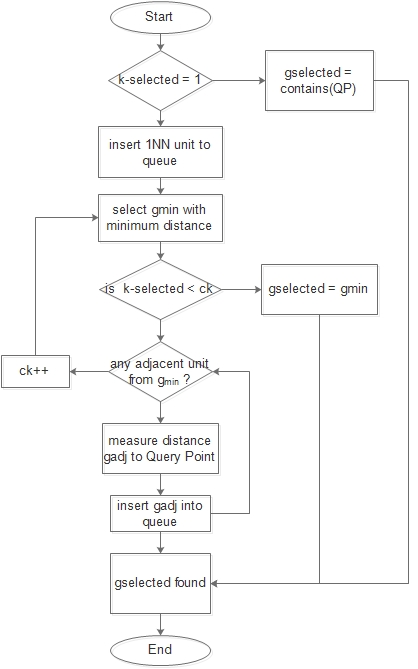
\includegraphics[scale=0.56]{flowchart_knn.jpg}
    \caption{Flowchart K-Nearest Emergency Unit Determination}
    \label{fig:bp_pol}
\end{figure}

\pagebreak
\subsubsection{3.3.3.2.4 Process of Determining Shortest Path from Selected Emergency Unit to Emergency Location}
\begin{enumerate}[label=Input\hspace{5mm} :\hspace{2mm}, leftmargin=*, topsep=0pt, itemsep=-1ex, parsep=1ex]
\item selected unit location, emergency location
\end{enumerate}
\begin{enumerate}[label=Output\hspace{2mm} :\hspace{2mm}, leftmargin=*, topsep=0pt, itemsep=-1ex, parsep=1ex]
\item nearest route
\end{enumerate}
This step used to send shortest path information to selected emergency units so they can immediately do first aid. It will reduce or even prevent fatal impact from emergency. These selected unit will becomes starting point and the emergency location will becomes end point. System will expanding road network and select vertex with minimum distance from starting point to end point.

\section{Analysis and Interpretation Data}
In this section, data analysis and interpretation of the results based on data collection and processing in the previous section. The purpose of this section is to provide clearer information about the results and able to provide solutions to emerging research problems.


\subsection{Analysis of NVD Construction}
Analysis of NVD construction results is used to determine coverage area of each emergency unit to determine nearest emergency unit from an emergency location.

\subsection{Analysis of NVD-based KNN Performance}
The result of k-nearest emergency unit analysis is done to show the performance of accuracy and execution time between NVD-based KNN and basic KNN in case determining k-nearest emergency unit.


\section{Conclusions and Suggestion}
The conclusions and suggestions step is the final step of this final project which contains the conclusions of the overall results and analysis that refers to the initial objectives. It also provides advice related to the development that can be built for further research.
%
\definecolor{gray}{gray}{0.75}

\chapter{Data Collection and Processing}
In this section will be described on the process of collecting and processing data and analysis results are performed in accordance with the methodology described in the previous discussion.

\section{Data Collection}
At this stage, data are collected. Its to support kth nearest neighbour and route determination model. The data collected are as follows:

\subsection{Bandung road network map}
Data collected consist of Bandung administrative map and road network. Bandung road network map covers national road, provincial road, city road and some environmental road. However, the road network used in this study is only a network of arterial and collector class roads. To facilitate the processing of road network data, also required data vertex dividing the road network obtained based on the existing intersections.

\begin{figure}[H]
    \centering
    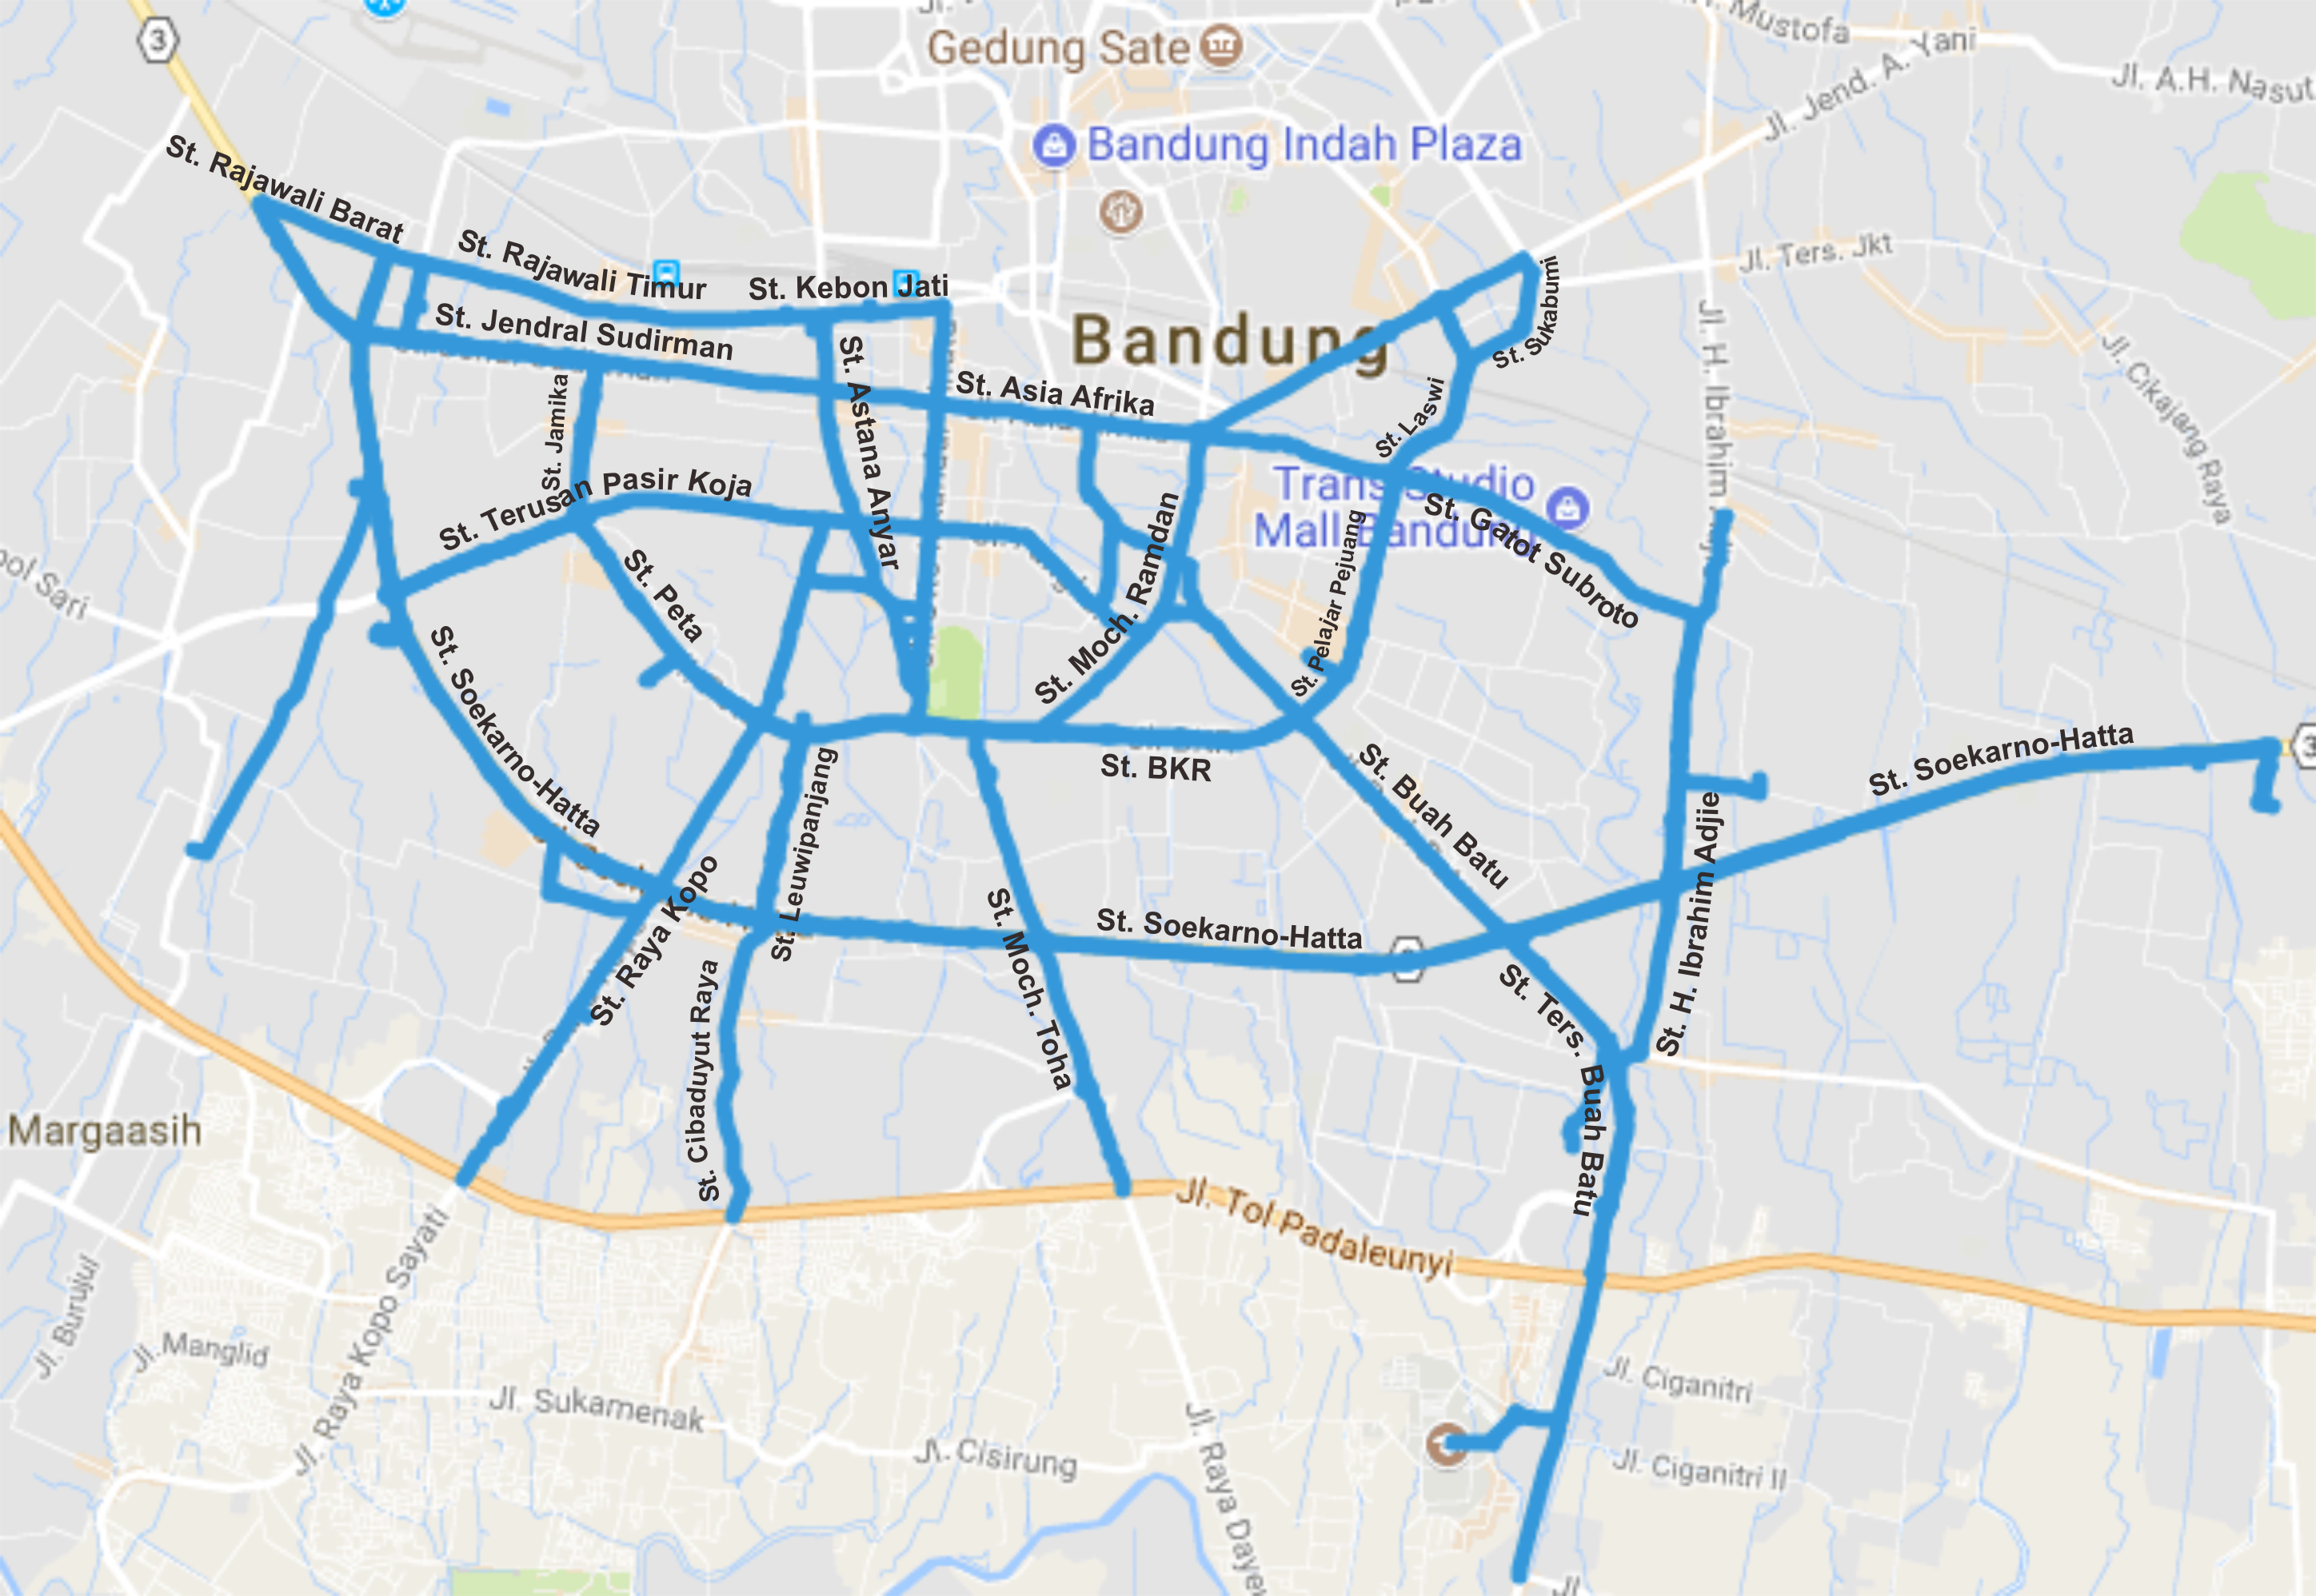
\includegraphics[scale=0.42]{data_coll1.png}
    \caption{Bandung administrative map}
    \label{fig:bandung_administrativ_map}
\end{figure}

\begin{table}[H] 
\centering
\begin{tabular}{|c|c|c|c|}
\hline
\rowcolor{gray}
\textbf{No} & \textbf{Name} & \textbf{Distance (km)} & \textbf{Status} \\
\hline
\multicolumn{2}{|l|}{\textit{Primary Artery Street}} &  & \\
\cline{1-4}
1. & \multicolumn{1}{|l|}{St. Jend. Sudirman} & 6,79 & National \\
\cline{1-4}
2. & \multicolumn{1}{|l|}{St. Asia Afrika} & 1,51 & National \\
\cline{1-4}
3. & \multicolumn{1}{|l|}{St. Soekarno-Hatta} & 18,46 & National \\

\cline{1-4}
\multicolumn{2}{|l|}{\textit{Secondary Artery Street}} &  & \\

\cline{1-4}
1. & \multicolumn{1}{|l|}{St. Peta} & 2,46 & Province \\
\cline{1-4}
2. & \multicolumn{1}{|l|}{St. BKR} & 2,30 & Province \\
\cline{1-4}
3. & \multicolumn{1}{|l|}{St. Pelajar Pejuang} & 1,56 & Province \\
\cline{1-4}
4. & \multicolumn{1}{|l|}{St. Laswi} & 1,17 & Province \\
\cline{1-4}
5. & \multicolumn{1}{|l|}{St. Gatot Subroto} & 1,68 & Province \\
\cline{1-4}
6. & \multicolumn{1}{|l|}{St. Jamika} & 0,91 & City \\
\cline{1-4}
7. & \multicolumn{1}{|l|}{St. Sukabumi} & 0,64 & City \\
\hline
\end{tabular}
\caption{Artery Road Data}
\label{table:street_data1}
\end{table}

\begin{table}[H] 
\centering
\begin{tabular}{|c|c|c|c|}
\hline
\rowcolor{gray}
\textbf{No} & \textbf{Name} & \textbf{Distance (km)} & \textbf{Status} \\
\hline
\multicolumn{2}{|l|}{\textit{Primary Collector Street}} &  & \\
\cline{1-4}
1. & \multicolumn{1}{|l|}{St. Pasir Koja} & 0,13 & Province \\
\cline{1-4}
2. & \multicolumn{1}{|l|}{St. Ters. Pasir Koja} & 2,72 & Province \\
\cline{1-4}
3. & \multicolumn{1}{|l|}{St. Raya Kopo} & 2,96 & Province \\
\cline{1-4}
4. & \multicolumn{1}{|l|}{St. Buah Batu} & 0,99 & Province \\
\cline{1-4}
5. & \multicolumn{1}{|l|}{St. Ters. Buah Batu} & 1,06 & Province \\
\cline{1-4}
6. & \multicolumn{1}{|l|}{St. H. Ibrahim Adjie} & 1,16 & Province \\
\cline{1-4}
7. & \multicolumn{1}{|l|}{St. Moch. Toha} & 3,47 & Province \\
\cline{1-4}
8. & \multicolumn{1}{|l|}{St. Leuwipanjang} & 1,08 & Province \\
\cline{1-4}
9. & \multicolumn{1}{|l|}{St. Cibaduyut Raya} & 1,72 & Province \\
\cline{1-4}
10. & \multicolumn{1}{|l|}{St. Astana Anyar} & 0,76 & City \\
\cline{1-4}
11. & \multicolumn{1}{|l|}{St. Moch. Ramdan} & 0,94 & City \\
\cline{1-4}
\multicolumn{2}{|l|}{\textit{Secondary Collector Street}} &  & \\
\cline{1-4}
1. & \multicolumn{1}{|l|}{St. Rajawali Barat} & 1,02 & Nasional \\
\cline{1-4}
2. & \multicolumn{1}{|l|}{St. Rajawali Timur} & 1,54 & Nasional \\
\cline{1-4}
3. & \multicolumn{1}{|l|}{St. Kebonjati} & 1,40 & Provinsi \\
\hline
\end{tabular}
\caption{Collector Road Data}
\label{table:street_data1}
\end{table}

\pagebreak

\subsection{Ambulance Location in Bandung}
The location point of the emergency unit in Bandung was obtained through field observation. Data coordinates the location of this emergency unit obtained from the Bandung data portal. Ambulance Location based on the coordinate point shown in figure \ref{fig:ambulance_location}
\begin{figure}[H]
    \centering
    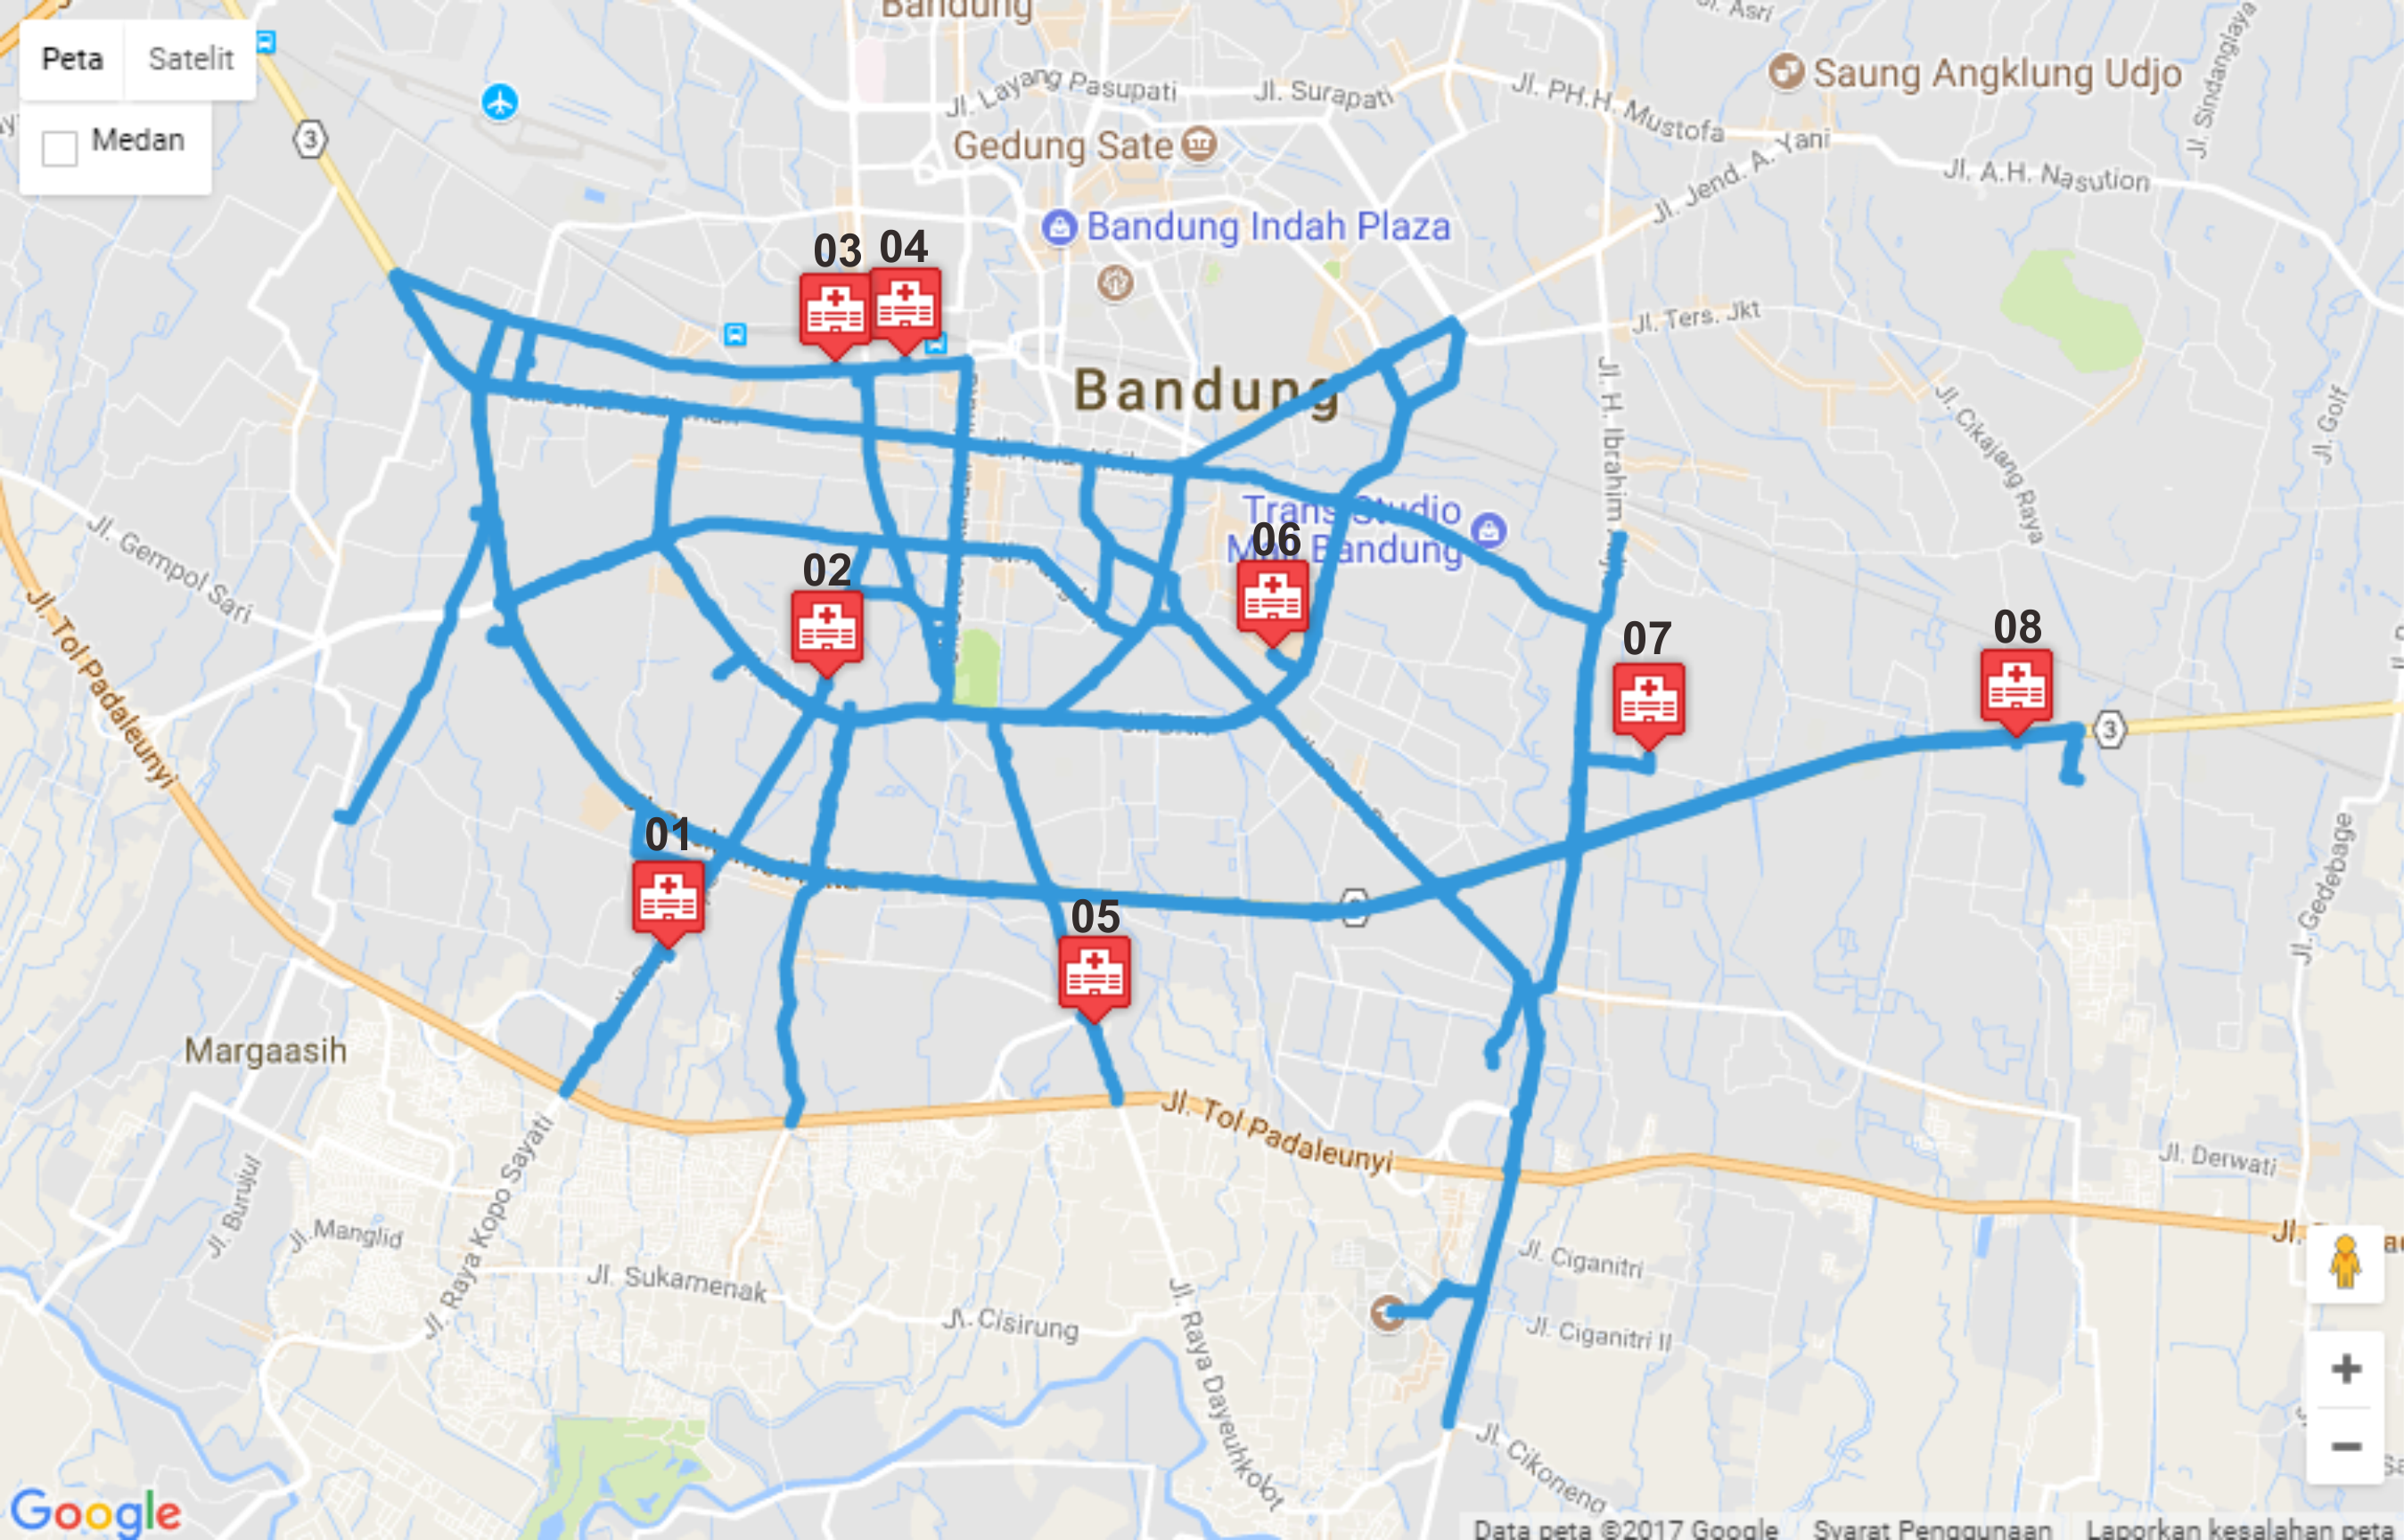
\includegraphics[scale=0.6]{data_coll2.png}
    \caption{Ambulance location in Bandung}
    \label{fig:ambulance_location}
\end{figure}

The symbols, captions, and coordinate points of figure \ref{fig:ambulance_location} are described in the table \ref{table:ambulance_data} below:

\begin{table}[H] 
\centering
\begin{tabular}{|c|c|c|c|c|}
\hline
\rowcolor{gray}
\textbf{No} & \textbf{Id} & \textbf{Name} & \textbf{Latitude} & \textbf{Longitude} \\
\hline
1. & AMB001 & \multicolumn{1}{|l|}{RSU Santosa Kopo} & -6.952198 & 107.586060 \\
\cline{1-5}
2. & AMB002 & \multicolumn{1}{|l|}{RSU Immanuel} & -6.935604 & 107.595856 \\
\cline{1-5}
3. & AMB003 & \multicolumn{1}{|l|}{RSU Kebonjati} & -6.916139 & 107.596306 \\
\cline{1-5}
4. & AMB004 & \multicolumn{1}{|l|}{RSU Santosa Bandung Central} & -6.915867 & 107.600533 \\
\cline{1-5}
5. & AMB005 & \multicolumn{1}{|l|}{RSU Sartika Asih} & -6.956771 & 107.612312 \\
\cline{1-5}
6. & AMB006 & \multicolumn{1}{|l|}{RSU Muhammadiyah} & -6.933718 & 107.623299 \\
\cline{1-5}
7. & AMB007 & \multicolumn{1}{|l|}{RSU KCK Pindad} & -6.939983 & 107.646523  \\
\cline{1-5}
8. & AMB008 & \multicolumn{1}{|l|}{RSU Al-Islam} & -6.939277 & 107.6691134 \\
\hline
\end{tabular}
\caption{Ambulance Data}
\label{table:ambulance_data}
\end{table}

\subsection{Police Location in Bandung}
The location point of the emergency unit in Bandung was obtained through field observation. Data coordinates the location of this emergency unit obtained from the Bandung data portal. Police Location based on the coordinate point shown in figure \ref{fig:police_location}

\begin{figure}[H]
    \centering
    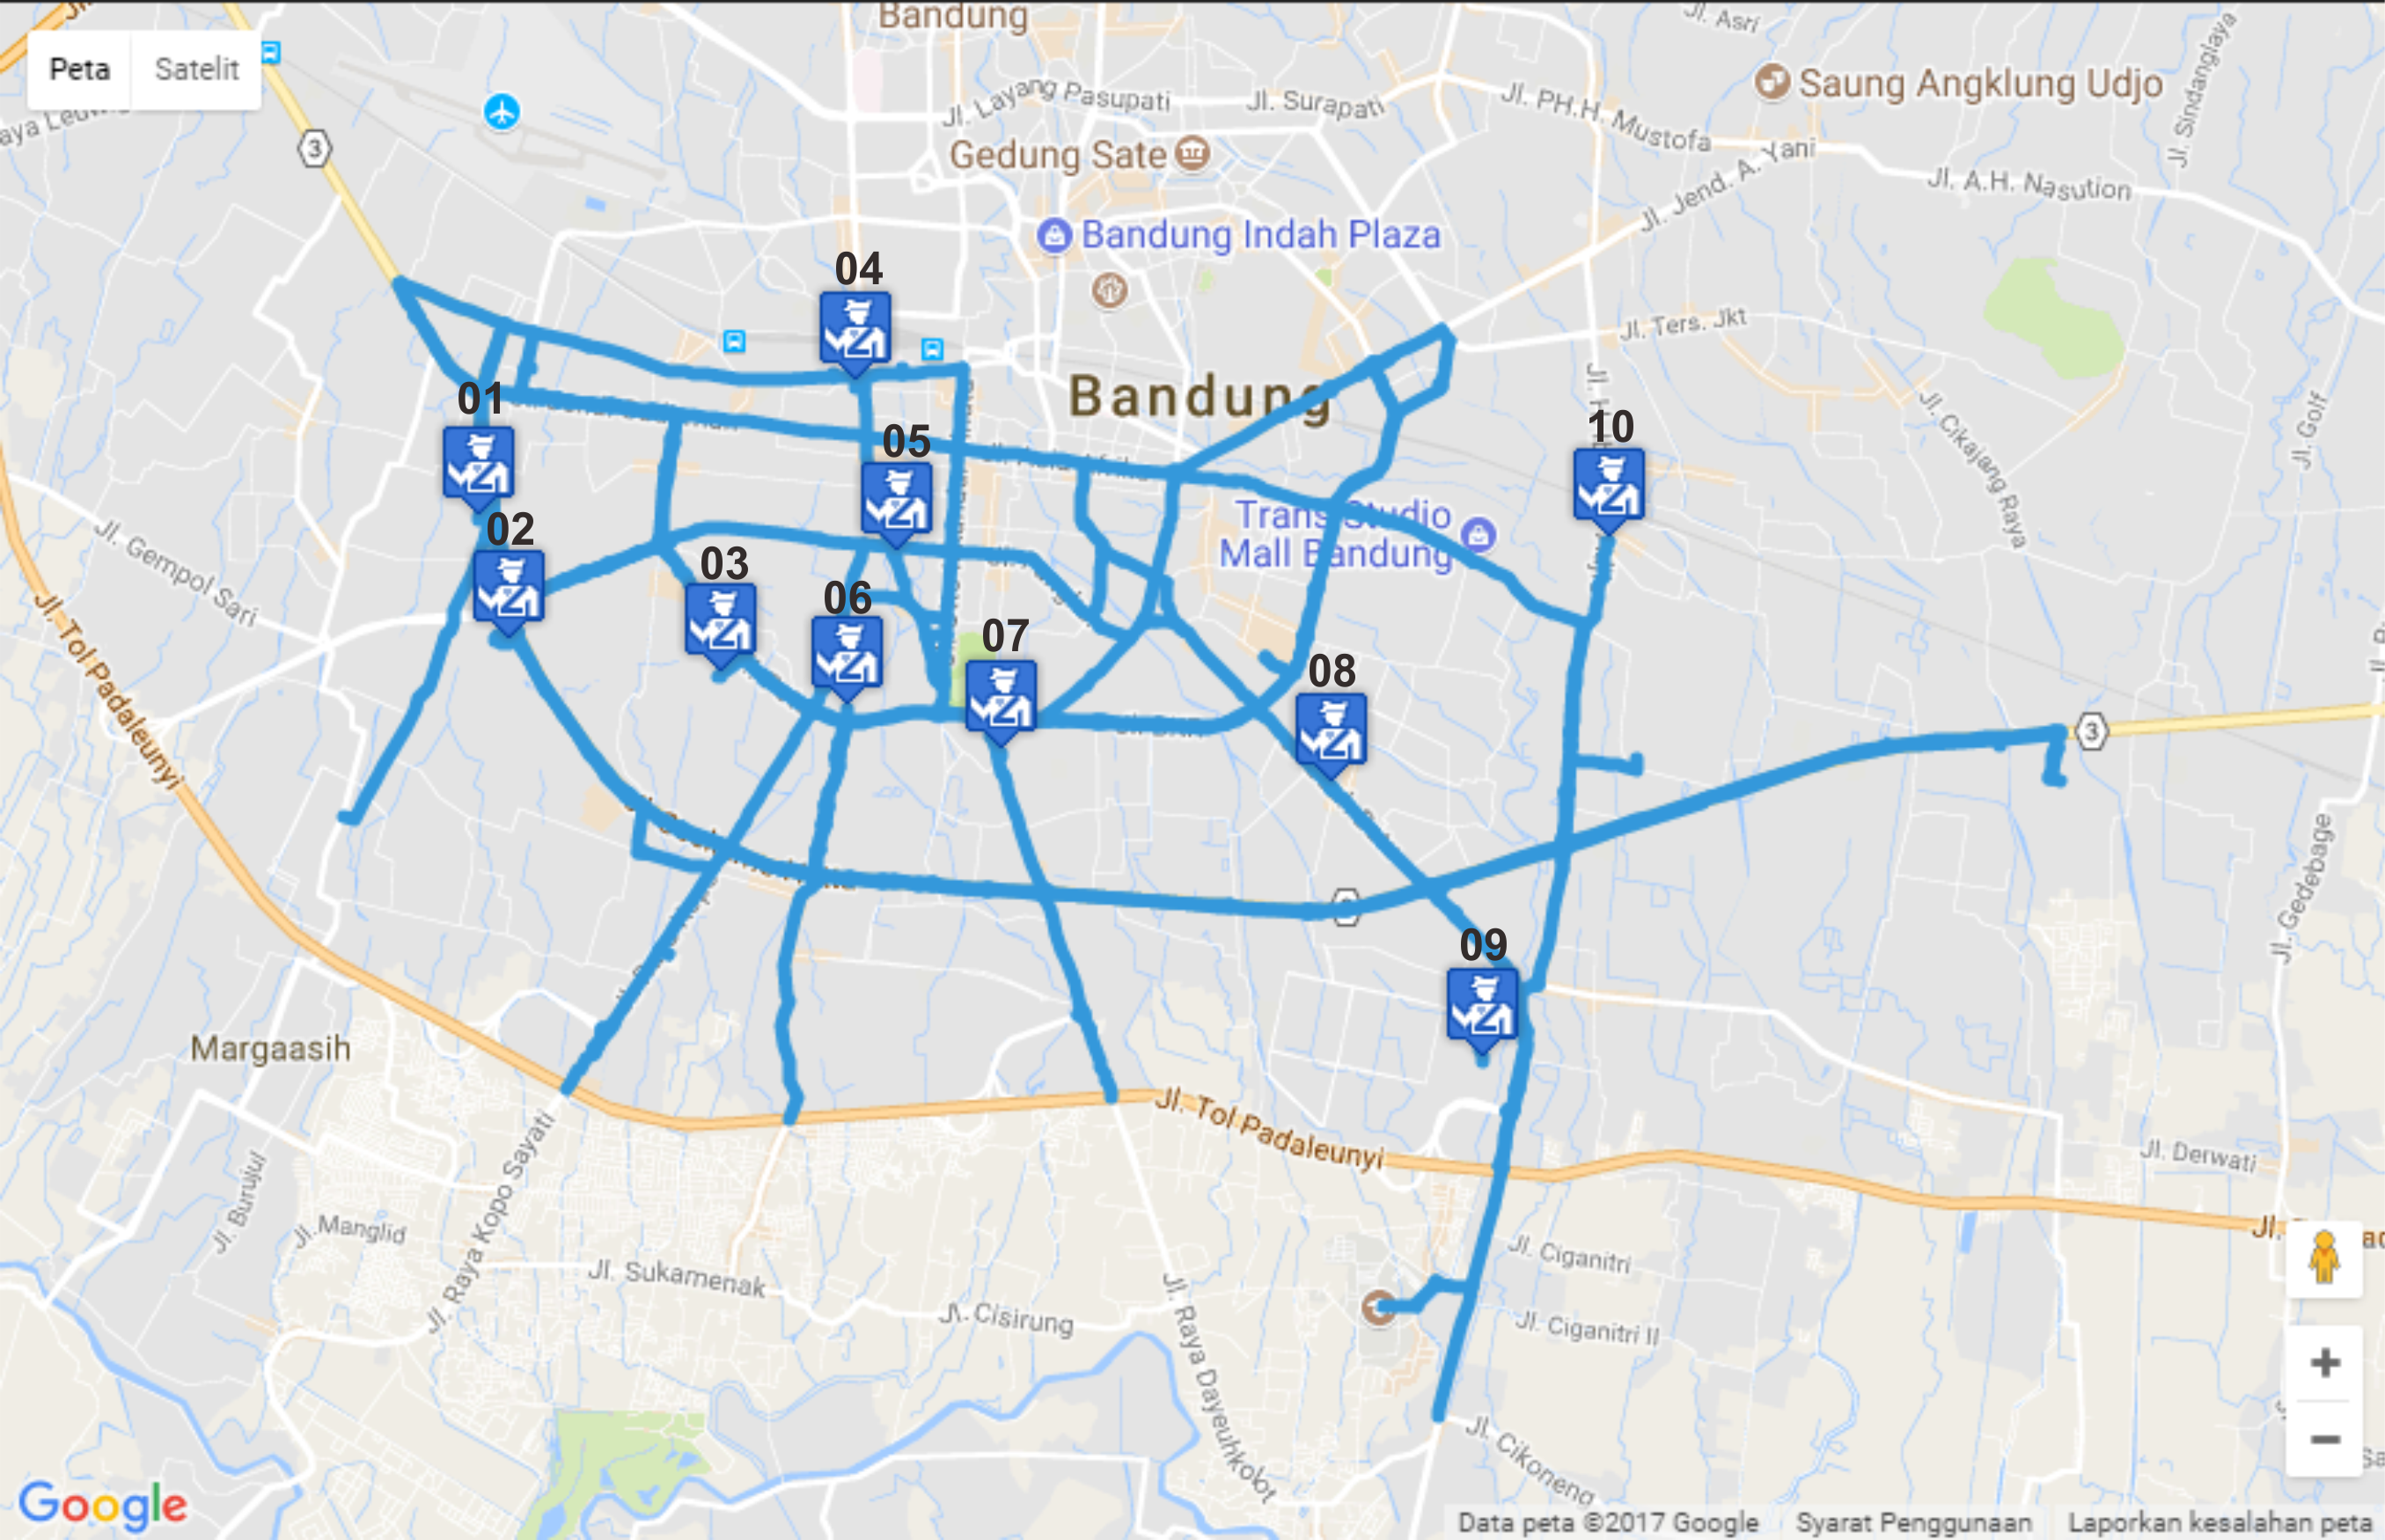
\includegraphics[scale=0.6]{data_coll3.png}
    \caption{Police location in Bandung}
    \label{fig:police_location}
\end{figure}

The symbols, captions, and coordinate points of figure \ref{fig:police_location} are described in the table \ref{table:police_data} below:

\begin{table}[H] 
\centering
\begin{tabular}{|c|c|c|c|c|}
\hline
\rowcolor{gray}
\textbf{No} & \textbf{Id} & \textbf{Name} & \textbf{Latitude} & \textbf{Longitude} \\
  \hline
1. & POL001 & \multicolumn{1}{|l|}{Polsek Bandung Kulon} & -6.925269 & 107.574158 \\
  \cline{1-5}
2. & POL002 & \multicolumn{1}{|l|}{Polsek Babakan Ciparay} & -6.932978 & 107.575981 \\
  \cline{1-5}
3. & POL003 & \multicolumn{1}{|l|}{Polsek Bojongloa Kaler} & -6.935009 & 107.589287 \\
  \cline{1-5}
4. & POL004 & \multicolumn{1}{|l|}{Polsek Andir} & -6.916926 & 107.597664 \\
  \cline{1-5}
5. & POL005 & \multicolumn{1}{|l|}{Polsek Astana Anyar} & -6.927466 & 107.600204 \\
  \cline{1-5}
6. & POL006 & \multicolumn{1}{|l|}{Polsek Bojongloa Kidul} & -6.937067 & 107.597115 \\
   \cline{1-5}
7. & POL007 & \multicolumn{1}{|l|}{Polsek Regol} & -6.939767 & 107.606819 \\
  \cline{1-5}
8. & POL008 & \multicolumn{1}{|l|}{Polsek Lengkong} & -6.941817 & 107.627449 \\
   \cline{1-5}
9. & POL009 & \multicolumn{1}{|l|}{Polsek Bandung Kidul} & -6.958753 & 107.636917  \\
   \cline{1-5}
10. & POL010 & \multicolumn{1}{|l|}{Polsek Kiaracondong} & -6.926602 & 107.644714 \\
  \hline
\end{tabular}
\caption{Police Data}
\label{table:police_data}
\end{table}


\subsection{Fire Brigade in Bandung}
The location point of the emergency unit in Bandung was obtained through field observation. Data coordinates the location of this emergency unit obtained from the Bandung data portal. Police Location based on the coordinate point shown in figure \ref{fig:fire_brigade_location}

\begin{figure}[H]
    \centering
    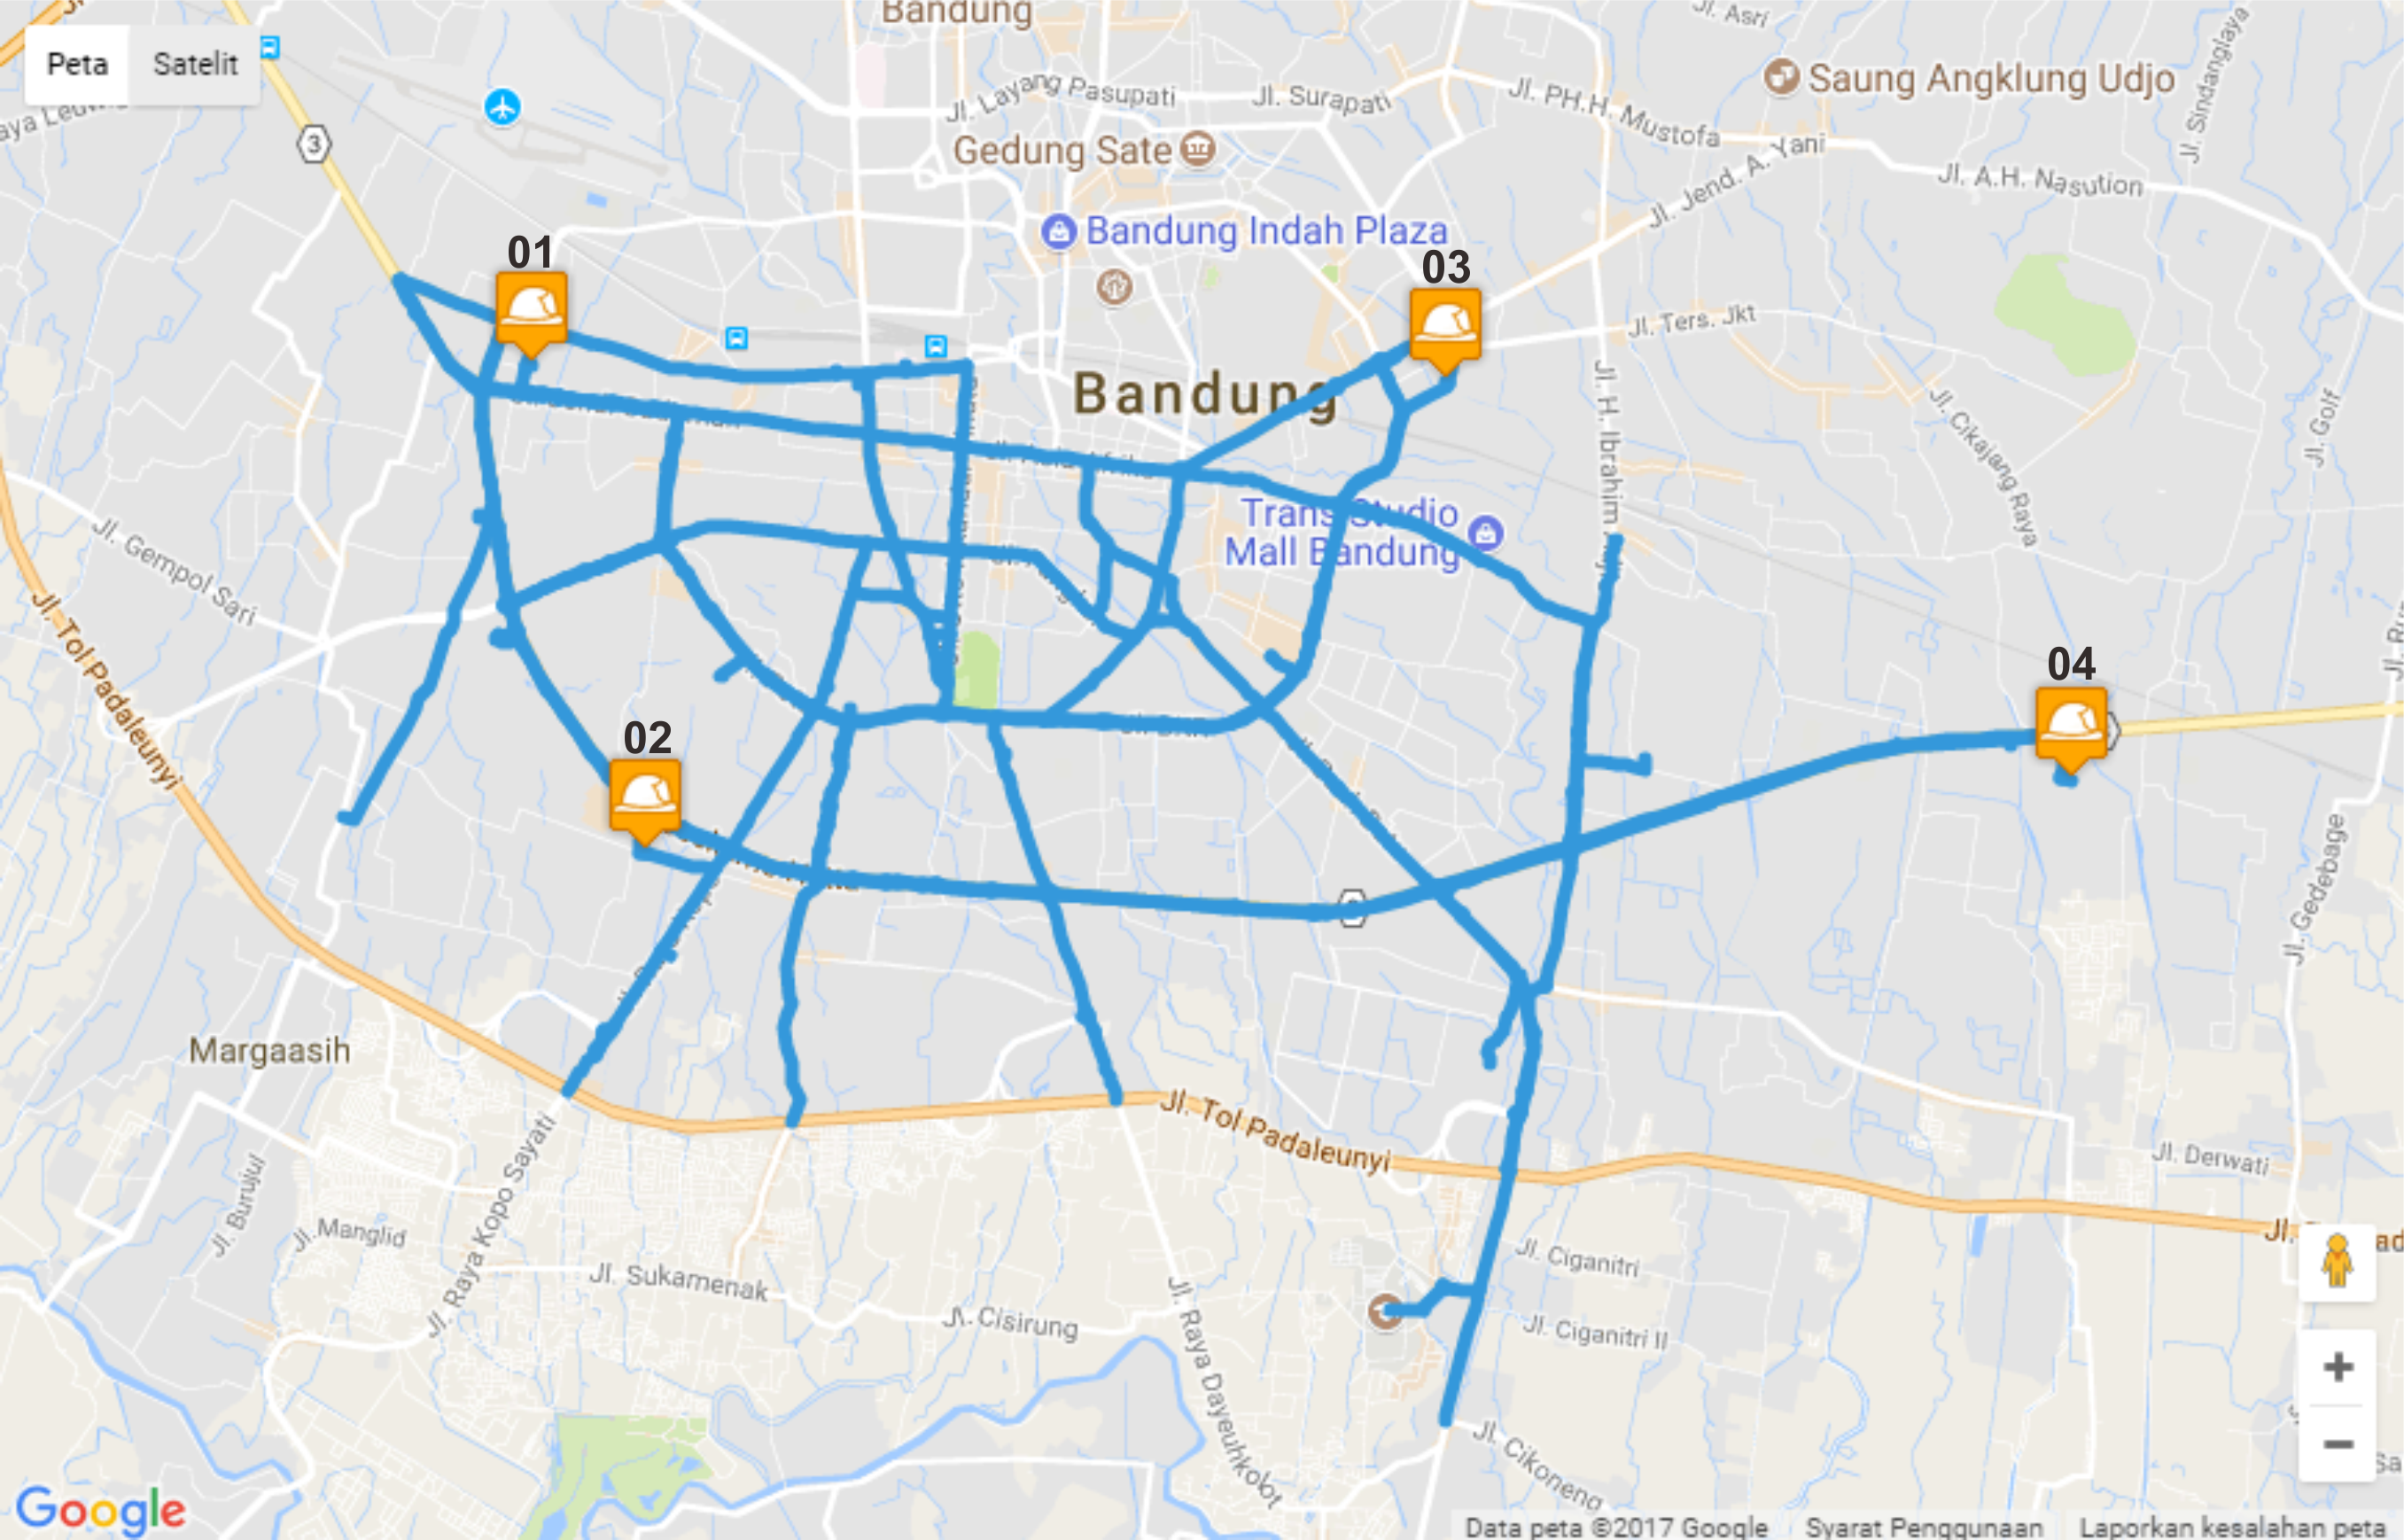
\includegraphics[scale=0.6]{data_coll4.png}
    \caption{Fire Brigade location in Bandung}
    \label{fig:fire_brigade_location}
\end{figure}

The symbols, captions, and coordinate points of figure \ref{fig:fire_brigade_location} are described in the table \ref{table:fire_brigade_data} below:

\begin{table}[H] 
\centering
\begin{tabular}{|c|c|c|c|c|}
\hline
\rowcolor{gray}
\textbf{No} & \textbf{Id} & \textbf{Name} & \textbf{Latitude} & \textbf{Longitude} \\
\hline
1. & FBR001 & \multicolumn{1}{|l|}{UPT Damkar Wilayah Barat} & -6.915912 & 107.577354 \\
\cline{1-5}
2. & FBR002 & \multicolumn{1}{|l|}{UPT Damkar Wilayah Selatan} & -6.945922 & 107.584412  \\
\cline{1-5}
3. & FBR003 & \multicolumn{1}{|l|}{Dinas Kebakaran Kota Bandung} & -6.916825 & 107.634109 \\
\cline{1-5}
4. & FBR004 & \multicolumn{1}{|l|}{UPT Damkar Wilayah Timur} & -6.941342 & 107.672874 \\
\hline
\end{tabular}
\caption{Fire Brigade Data}
\label{table:fire_brigade_data}
\end{table}

\pagebreak

\section{Data Processing}
Data processing is done to get the nearest generator from query point and calculate optimal route from the generator to the query point based on the shortest route. In this case, a nearby generator search is made up of units such as police, ambulance, and fire brigade. Then calculate optimal route from selected units to the query point which is the scene of the accident.

\subsection{Constructing Network Voronoi Diagram}
This step intended to divides road network into subnetworks which are act as a coverage area for an emergency unit. These coverage area always returns its generator for nearest emergency unit. This step consists two following process which are border point determination and nearest emergency unit classification.

\subsubsection{- Determining Border Point}
This step intended to determine the border point between adjacent units by expanding each unit so that each unit has at least been a starting point. Expansion is done using queue which sorted by minimum distance. The following example presents an example of data processing to get the border points of the RSU Al-Islam to its neighbor generator.

\begin{figure}[H]
    \centering
    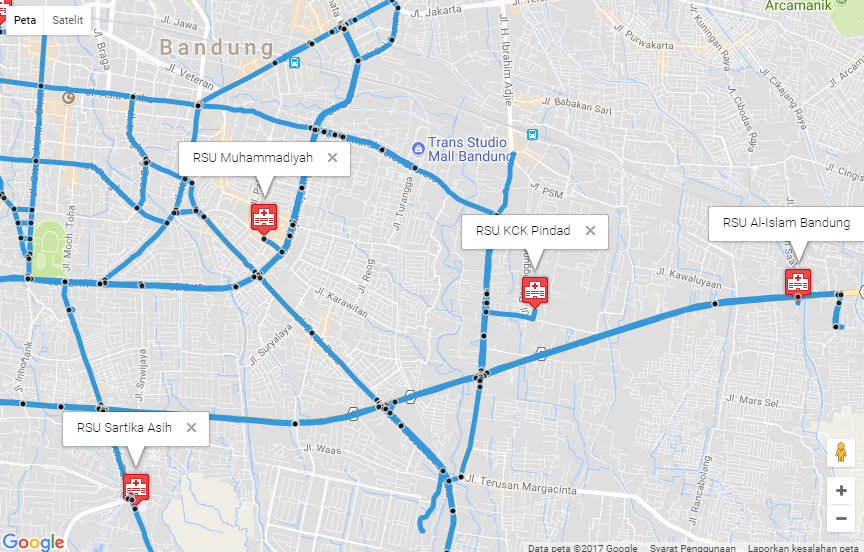
\includegraphics[scale=0.53]{data_proc_1_1.png}
    \caption{RSU Al-Islam Map}
    \label{fig:rsu_al-islam_map}
\end{figure}

\begin{table}[H]
\centering
\begin{tabular}{lll}
Id Vertex & = & 20           \\
Name      & = & RSU Al-Islam \\
Unit Type & = & Ambulance   
\end{tabular}
\end{table}

Vertex 20 inserted into the queue and act as $v_{selected}$. For each vertex that shares same edge with vertex 20 will be checked its type. So expanding process when meets another generator RSU KCK Pindad is shown in \ref{fig:alur_expand} below:

\begin{figure}[H]
    \centering
    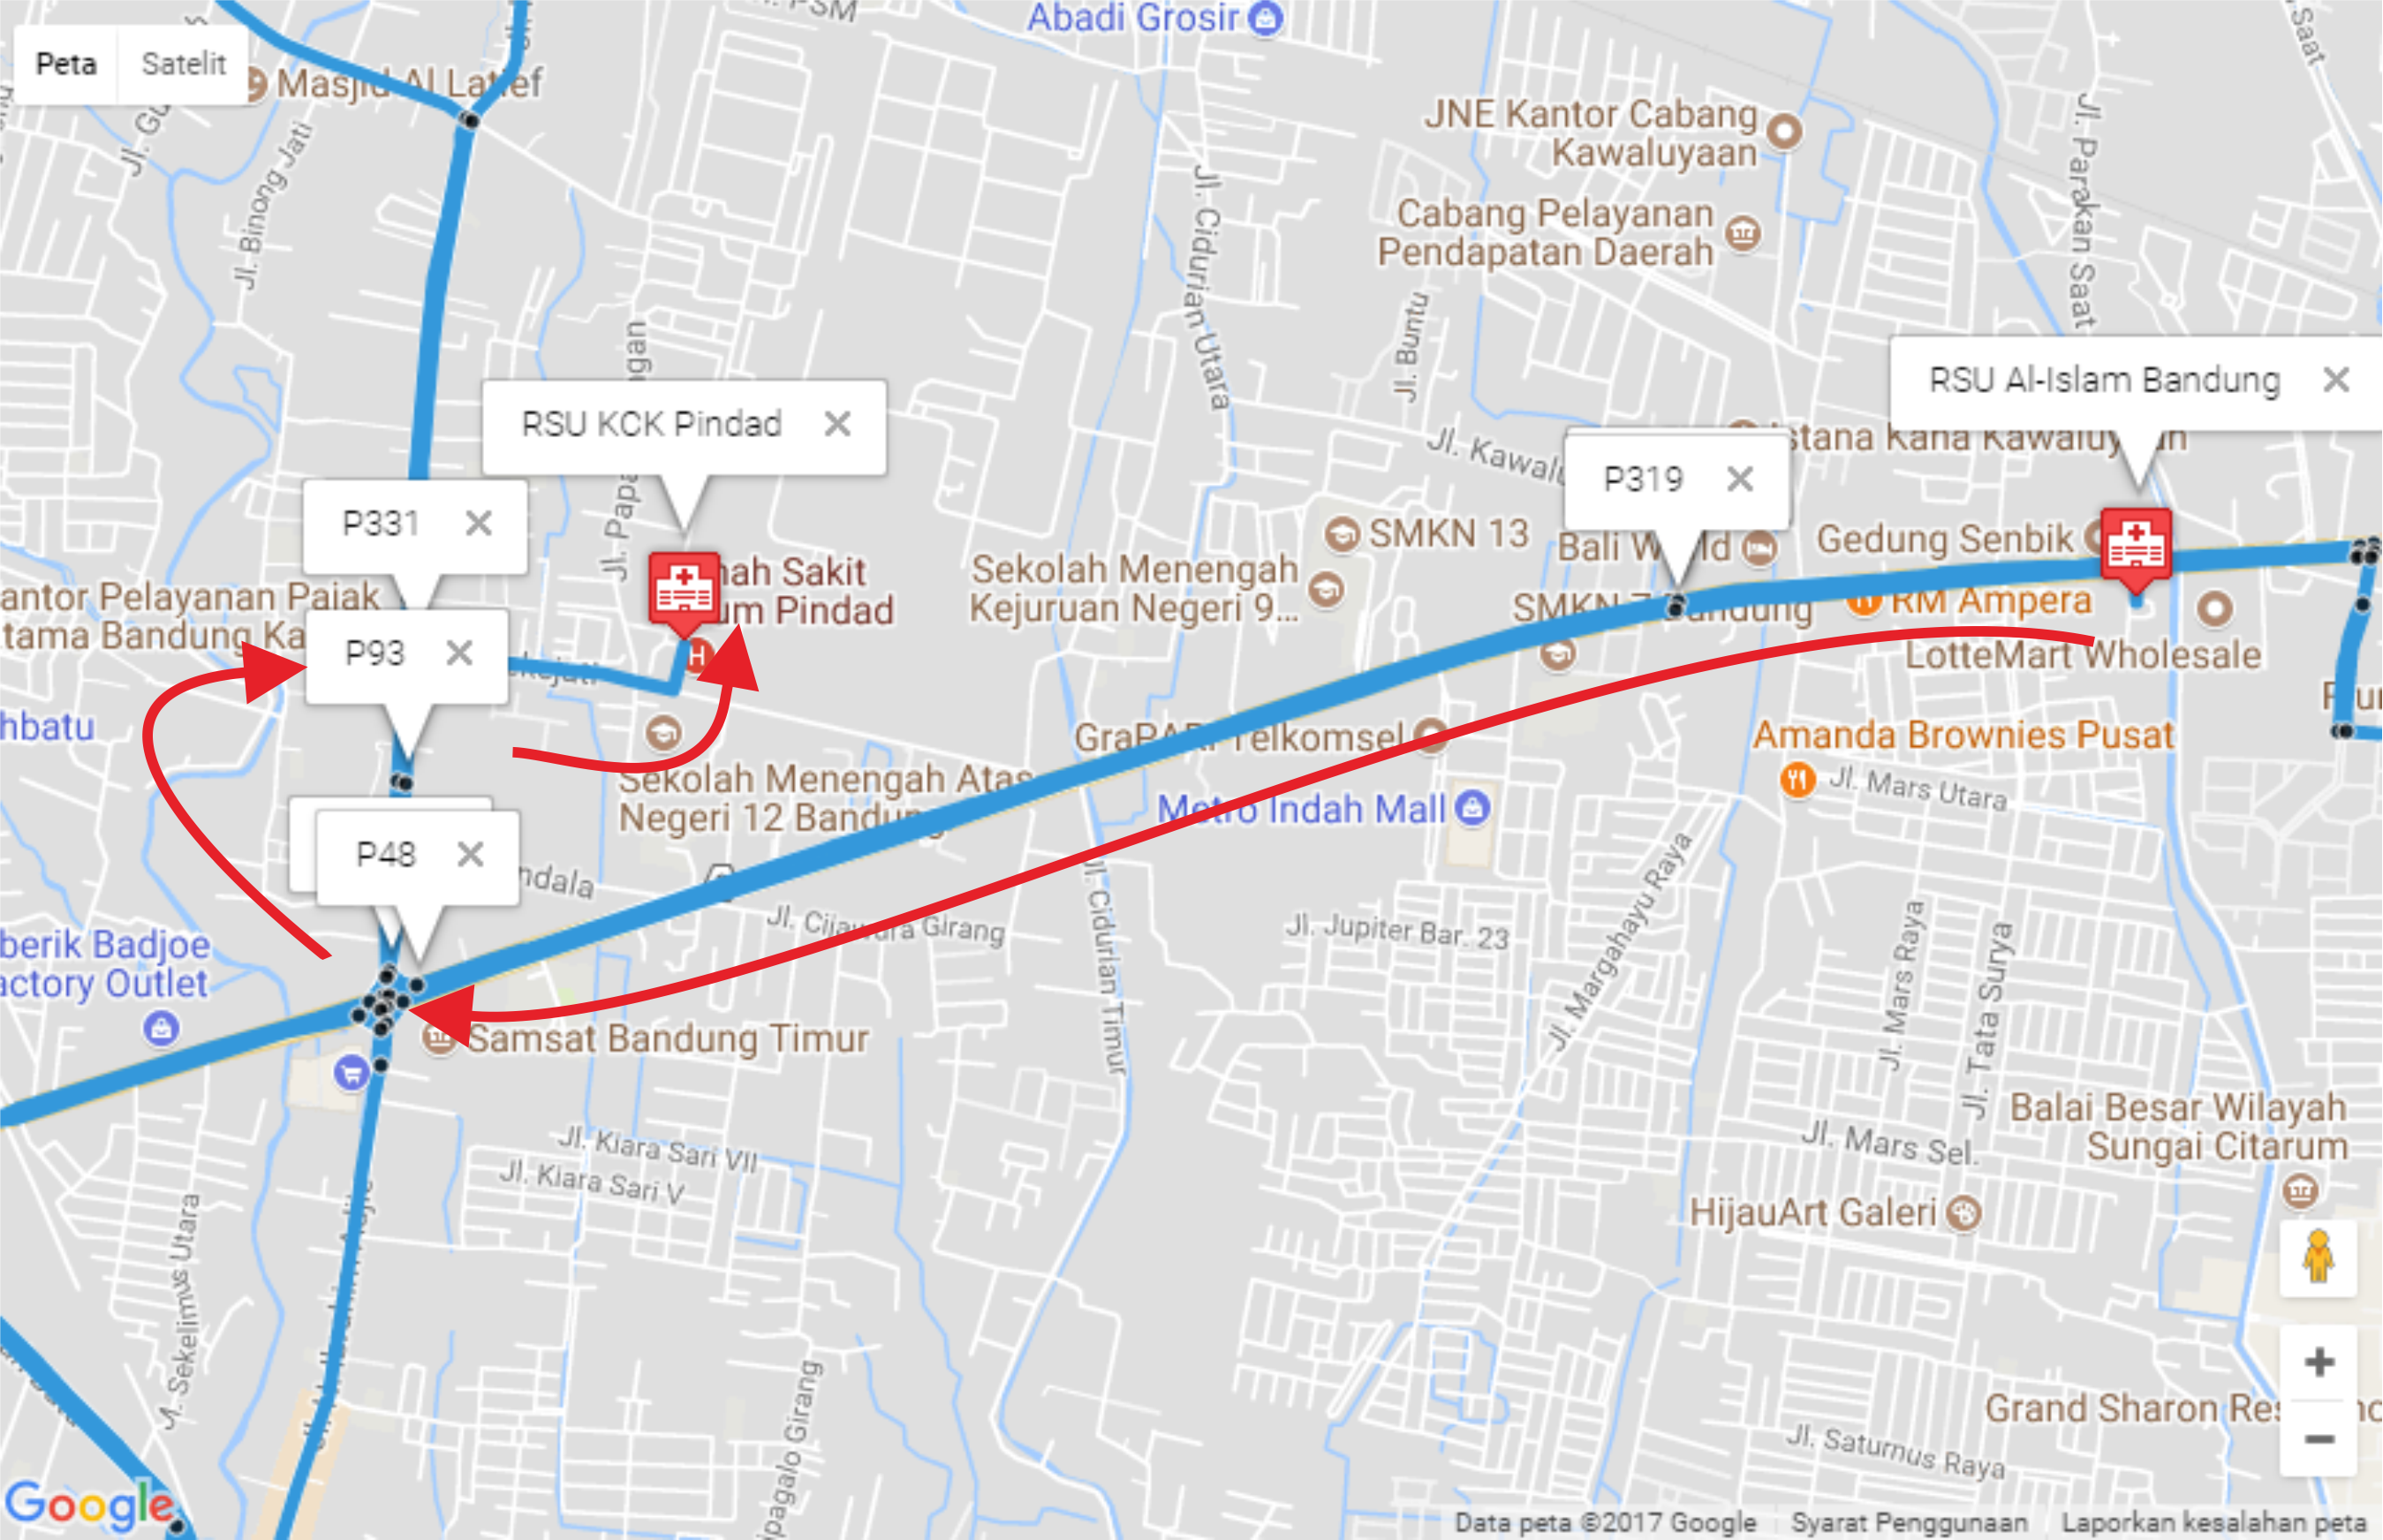
\includegraphics[scale=0.55]{data_proc_1_2.png}
    \caption{Expansion Flow of RSU Al-Islam Hospital to RSU KCK Pindad}
    \label{fig:alur_expand}
\end{figure}

\begin{table}[H]
\begin{tabular}{lll}
Path & = & 322-323-318-48-49-93-331-330 \\
Total Distance & = & 4.2903026796279 km\\
\end{tabular}
\end{table}

From the path data, border points can be obtained by determine middle distance from RSU Al-Islam and RSU KCK Pindad as follows:

\begin{table}[H]
\begin{tabular}{lll}
Mid Distance & = & 2,14515 km \\
Subdistance & = & 0,048559089918396 km\\
Edge Selected & = & N48N318\\
 & &\\
Edge Point 1 Id  & = & N48N318-08\\
Edge Point 1 Latitude & = & -6.943101\\
Edge Point 1 Longitude & = & 107.648819\\
 & &\\
Edge Point 2 Id  & = & N48N318-07\\
Edge Point 2 Id  & = & -6.942309\\
Edge Point 2 Id  & = & 107.651390\\
\end{tabular}
\end{table}

After that, calculation of the border point needs to determine its exact coordinates.

\begin{table}[H] 
\begin{tabular}{lll}
$fp$ & = & $subDistance / distance_{edgepoint2}$ \\
$fp$ & = & $0.048559089918396 / 0.299476$ \\
$fp$ & = & $0.16214684955855$ \\
\end{tabular}
\end{table}

\begin{table}[H] 
\begin{tabular}{lll}
$Lat_{mid}$ & = & $(Lat_{edgepoint2} \times (1-fp)) + (Lat_{edgepoint1} \times fp)$ \\
$Lat_{mid}$ & = & $(-6.943101 \times (1-0.16214)) + (-6.942309 \times 0.16214)$ \\
$Lat_{mid}$ & = & $-6.9424374203049$ \\
 & & \\
$Long_{mid}$ & = & $(Long_{edgepoint2} \times (1-fp)) + (Long_{edgepoint1} \times fp)$ \\
$Long_{mid}$ & = & $(107.651390 \times (1-0.16214)) + (107.648819 \times 0.16214)$ \\
$Long_{mid}$ & = & $107.6509731204$ \\
\end{tabular}
\end{table}

So the border point coordinates between RSU Al-Islam and RSU KCK Pindad is shown in \ref{fig:rsu_border_point} below:

\begin{figure}[H]
    \centering
    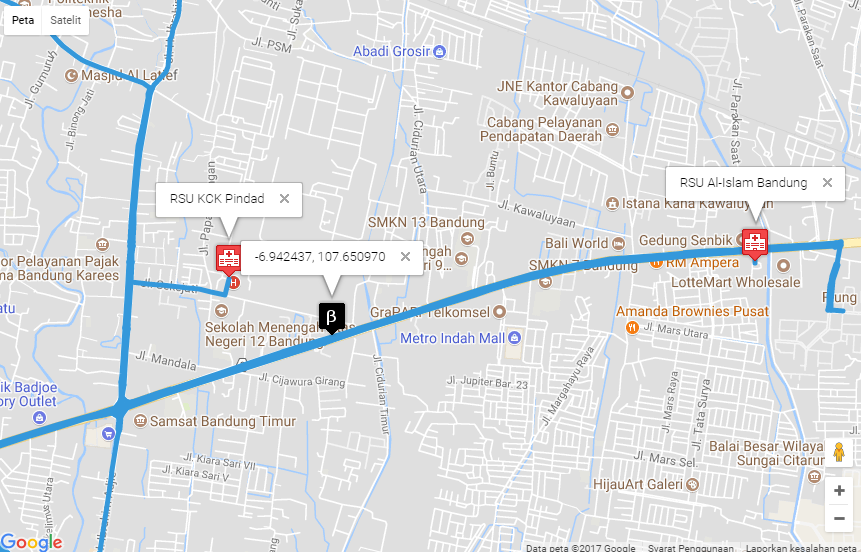
\includegraphics[scale=0.55]{data_proc_1_3.png}
    \caption{Border Point 441 Location}
    \label{fig:rsu_border_point}
\end{figure}

\begin{table}[H]
\centering
\begin{tabular}{lcl}
Id Vertex & =                     & 441              \\
Latitude  & =                     & -6.9424374203049 \\
Longitude & \multicolumn{1}{l}{=} & 107.65097312045 
\end{tabular}
\end{table}

\pagebreak

\subsubsection{- Classifying Nearest Emergency Unit}
The construction of network voronoi diagram is done by classifying nearest generator of all vertices. So network voronoi diagram will generating the coverage area of each generator which always returns its generator for nearest emergency unit. The following example shows the classification of the nearest ambulance generator of a vertex. Data attributes to be classified are as follows:

\begin{figure}[H]
    \centering
    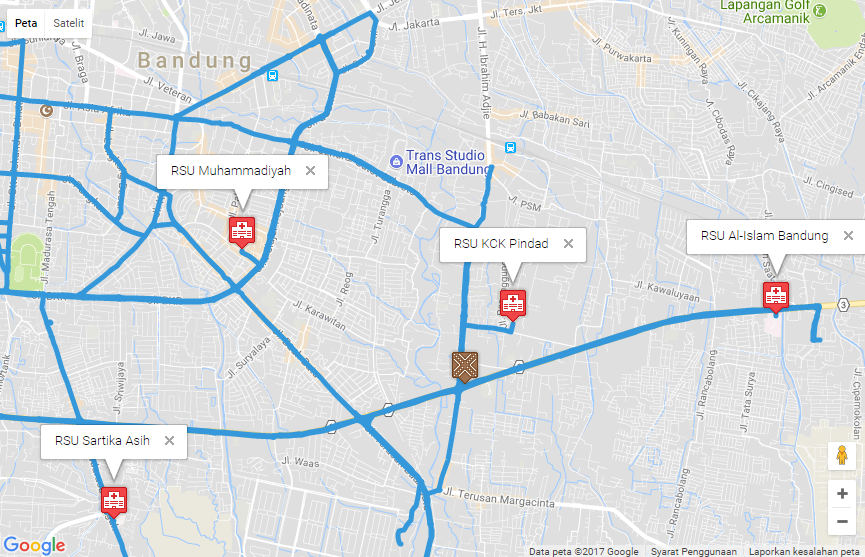
\includegraphics[scale=0.55]{data_proc_nvd_construction_1.png}
    \caption{Vertex 48 Location}
    \label{fig:rsu_border_point}
\end{figure}

\begin{table}[H]
\centering
\begin{tabular}{lll}
Id Vertex & = & 48 \\
Latitude & = & -6.945233 \\
Longitude & = & 107.642380 \\
\end{tabular}
\end{table}

Initialization queue is done first by entering data of each ambulance unit. Queue is sorted by the minimum distance to the emergency location (QP). After the insertion, the contents of queue are shown as follows.

\begin{table}[H] 
\centering
\begin{tabular}{|c|c|l|c|}
\hline
\textbf{No} & \textbf{$v_{id}$} & \textbf{$v_{data}$} & \textbf{$v_{distance}$}\\
\hline
1 &  322 & 322 (RSU Al-Islam Bandung) & 0\\
\hline
2 & 322 & 324 (RSU Kebonjati) & 0\\
\hline
3 & 328 & 328 (RSU Santosa Bandung Central) & 0\\
\hline
4 & 330 & 330 (RSU KCK Pindad) & 0\\
\hline
5 & 332 & 332 (RSU Sartika Asih) & 0\\
\hline
6 & 334 & 334 (RSU Santosa Bandung Kopo) & 0\\
\hline
7 & 336 & 336 (RSU Immanuel) & 0\\
\hline
8 & 338 & 338 (RSU Muhammadiyah Bandung) & 0\\
\hline
\end{tabular}
\caption{Queue initialization for Classifying 1NN}
\label{table:queue_inisialization}
\end{table}

Next iteration done with condition as long as queue is not empty. In each iteration $v_ {min}$ is extracted from queue which has minimum distance. For example, on the first iteration, the $v_{min}$ data obtained are shown as follows:

\begin{table}[H]
\begin{tabular}{lll}
$vmin_{id}$ & = & 49 \\
$vmin_{data}$ & = & 330 \\
$vmin_{distance}$ & = & 1,0821657 \\
\end{tabular}
\end{table}

From the $v_{min}$ data, then a $w$ search that shares the same edge with $v_ {min}$. Since $v_ {min}$ is selected adjacent with the vertex we want to classify, then $w$ data will we do the processing based on the vertex data you want to classify previously. So obtained the total distance as follows:

\begin{table}[H]
\begin{tabular}{lll}
$\Delta$ & = & $vmin_{distance}$ + distance($vmin{id}, w$) \\
$\Delta$ & = & 1,0821657 + 0,0569186 \\
$\Delta$ & = & 1,1390843 km \\
\end{tabular}
\end{table}


After getting the total distance to $w$, checks the condition of the meet. If $(w, v)_{distance} > \Delta$, then $(w, v)_{distance} \gets \Delta$ and reduce $(w, v)$ distance. But if $(w, v) \notin PQ$, then $(w, v)_{distance} \gets \Delta $ and $(w, v)$ inserted into queue.

\pagebreak
These steps are done continuously as long as queue condition is not empty. The result for vertex 48 on queue shown as follows:

\begin{figure}[H]
    \centering
    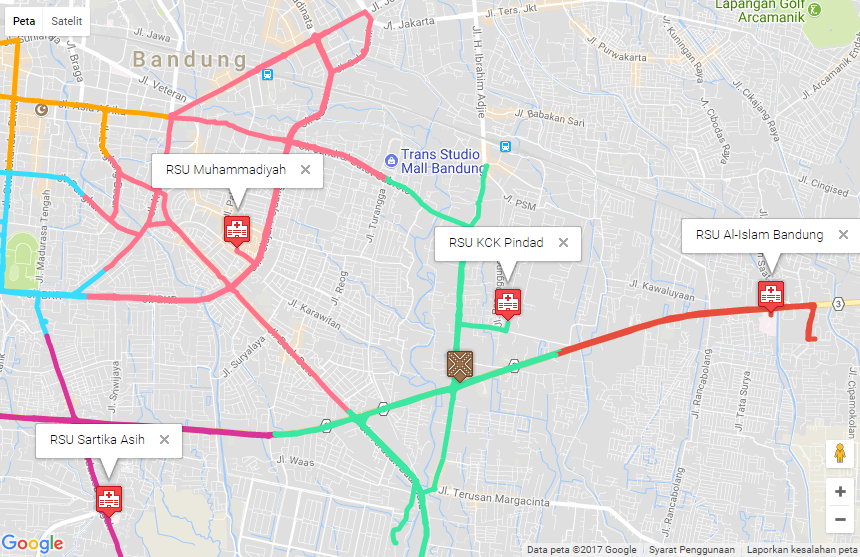
\includegraphics[scale=0.55]{data_proc_nvd_construction_2.png}
    \caption{Nearest Emergency Unit from Vertex 48}
    \label{fig:nn_vertex_48}
\end{figure}

\begin{table}[H]
\centering
\begin{tabular}{lll}
$v_{id}$       & = & 48                   \\
$v_{data}$     & = & 330 (RSU KCK Pindad) \\
$v_{distance}$ & = & 1.1390843           
\end{tabular}
\end{table}


\subsection{Determining Emergency Location}
This step is the process of determining coordinate point of emergency location. The location point of the emergency  will be the destination of the route to which selected emergency units assigned. The process of determining the location point of the incident is done by providing data in the form of latitude and longitude of the location. The location data of the emergency denote as query point (QP).

\pagebreak
For example, the determination of the location point of an emergency is shown as follows:

\begin{figure}[H]
    \centering
    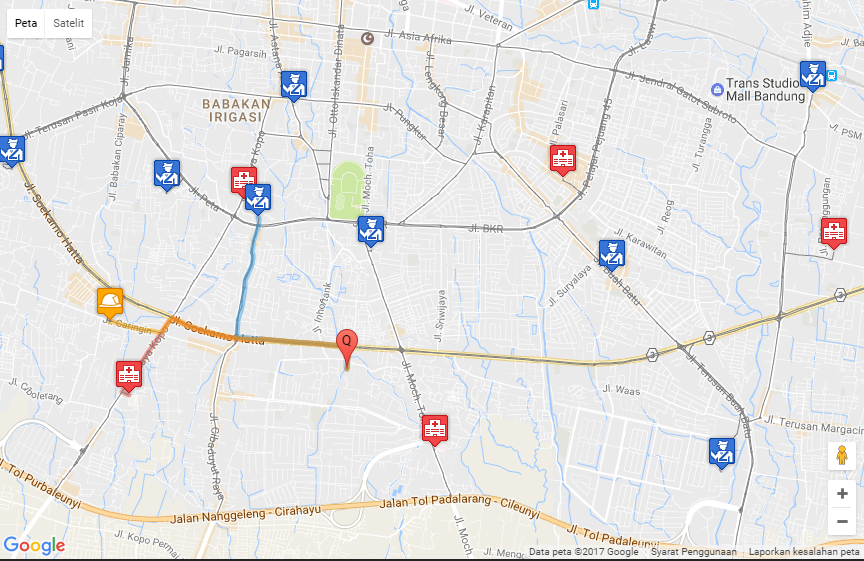
\includegraphics[scale=0.55]{data_proc_1.png}
    \caption{Emergency Location Coordinate}
    \label{fig:emergency_location_coordinate}
\end{figure}

\begin{table}[]
\centering
\begin{tabular}{lll}
Location  & = & Soekarno Hatta St. No. 396 D \\
Latitude  & = & -6.949942641719169           \\
Lomgitude & = & 107.6047620177269           
\end{tabular}
\end{table}


\subsection{Determining K-Nearest Unit to Emergency Location}
In this step, NVD-based KNN algorithms used to determining of k-nearest emergency unit. As an example of implementing the algorithm, suppose there is a query point (QP) in the form of emergency site location shown as following:

\begin{table}[H]
\centering
\begin{tabular}{lll}
Latitude   & = & -6.949942641719169 \\
Longitude  & = & 107.6047620177269  \\
Type Unit  & = & Ambulance          \\
K-Selected & = & 3                 
\end{tabular}
\end{table}

\pagebreak
NVD-based KNN algorithm requires network data voronoi diagram with k = 1 which has been done at nvd construction step. So that way, RSU Sartika Asih is the nearest emergency unit. The ambulance data inserted into the queue which sorted by the minimum distance shortest path as shown as follows:

\begin{table}[H] 
\centering
\begin{tabular}{|c|c|c|c|}
\hline
\textbf{No} & \textbf{Id} & \textbf{Name} & \textbf{Distance} \\
\hline
1 &  332 & RSU Sartika Asih & 1.6395278794745\\
\hline
\end{tabular}
\caption{Queue Initialization for Determining K-Nearest Emergency Unit}
\label{table:pq_initialization_3}
\end{table}

Furthermore, it is repeated with conditions for k obtained less or equal to the number of inputs k for this case k = 3. In each iteration $ v_ {min} $ selected by extracting emergency unit from queue which has minimum distance to emergency location (QP). Based on queue condition, the $ v_ {min} $ data obtained are as follows:

\begin{table}[H]
\centering{
\begin{tabular}{lll}
Id Generator & = & 332 \\
Name & = & RSU Sartika Asih \\
Distance & = & 1.6395278794745 \\
\end{tabular}}
\end{table}

Then, for every adjacent generator from $v_ {min}$ will be denoted as ($g_ {adj}$). Each $g_ {adj}$ inserted into queue and re-sorted queue by distance to QP. The result of inserting all $g_ {adj}$ from $v_ {min}$ is shown as follows:

\begin{table}[H] 
\centering
\begin{tabular}{|c|c|c|c|}
\hline
\textbf{No} & \textbf{Id} & \textbf{Name} & \textbf{Distance} \\
\hline
1 &  336 & RSU Immanuel & 2.531931093101\\
\hline
2 &  330 & RSU KCK Pindad & 5.4464306765158\\
\hline
\end{tabular}
\caption{PQ after Vertex 332's $g_{adj}$ inserted}
\label{table:tblhospital}
\end{table}

Then for k = 2 looping is done again. So based on queue above $v_min$ obtained as follows:

\begin{table}[H]
\centering{
\begin{tabular}{lll}
Id Generator & = & 336 \\
Name & = & RSU Immanuel \\
Distance & = & 2.531931093101 \\
\end{tabular}}
\end{table}

From the data $v_ {min}$ is done another search for $g_ {adj}$ which adjacent with $v_ {min}$. The result of inserting all $g_ {adj}$ from $v_ {min}$ is shown as follows:

\begin{table}[H] 
\centering
\begin{tabular}{|c|c|c|c|}
\hline
\textbf{No} & \textbf{Id} & \textbf{Name} & \textbf{Distance} \\
\hline
1 &  334 & RSU Immanuel & 2.6146168326924\\
\hline
2 &  338 & RSU Muhammadiyah Bandung & 4.2866445278889\\
\hline
2 &  324 & RSU Kebonjati & 4.8944211548207\\
\hline
2 &  328 & RSU Santosa Bandung Central & 4.9535388884729\\
\hline
2 &  330 & RSU KCK Pindad & 5.4464306765158\\
\hline
\end{tabular}
\caption{Hospital Data}
\label{table:tblhospital}
\end{table}

Due to the amount of looping has equal to value k which is 3, then based on queue the 3rd-nearest emergency unit shown as follows:

\begin{figure}[H]
    \centering
    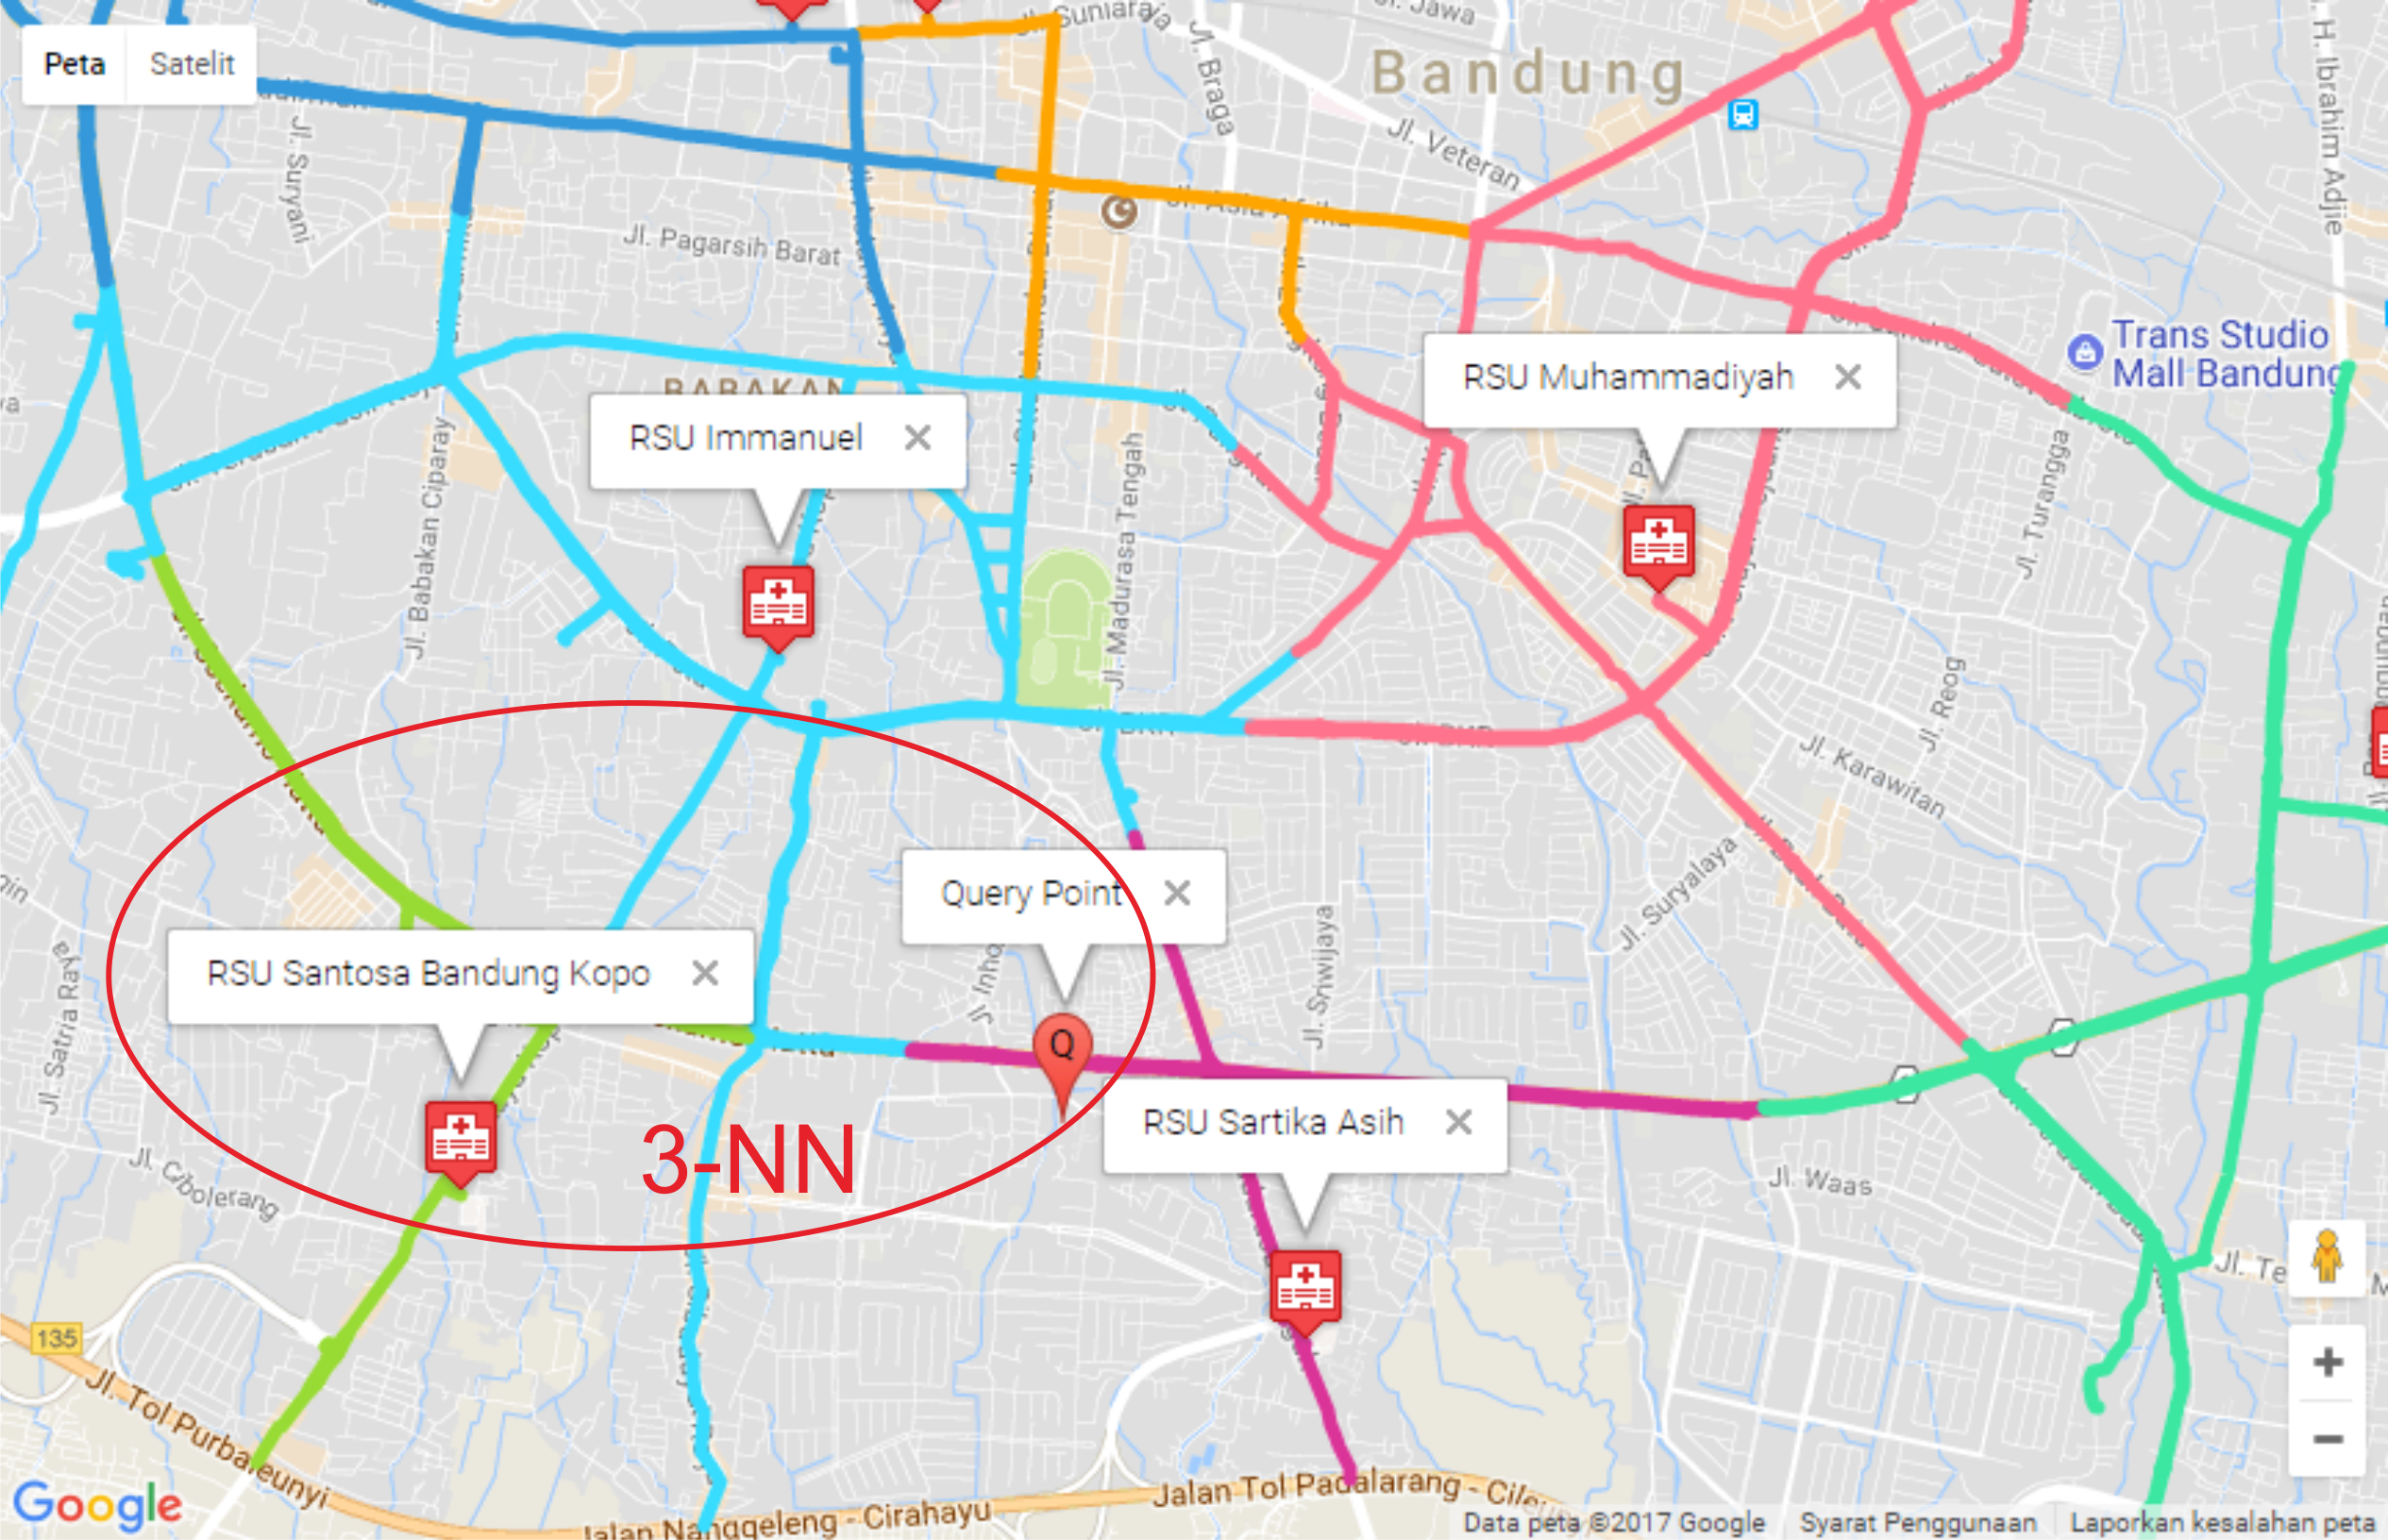
\includegraphics[scale=0.55]{data_proc_nvd-based_knn_3.png}
    \caption{3rd-Nearest Emergency Unit from QP}
    \label{fig:emergency_location_coordinate}
\end{figure}

\begin{table}[H]
\centering{
\begin{tabular}{lll}
Id Generator & = & 334 \\
Name & = & RSU Santosa Bandung Kopo \\
Latitude & = & -6.952198 \\
Longitude & = & 107.586060 \\
Type Unit & = & Ambulance \\
\end{tabular}}
\end{table}

\pagebreak
\subsection{Determining Shortest Path from Selected Emergency Unit to Emergency Location}
This step are based on the emergency location and selected units based on the previous step. The following are the data required for determining route from selected unit to emergency location:
\begin{table}[H]
\centering{
\begin{tabular}{lll}
Emergency Location & = & Jl. Soekarno Hatta \\
Latitude & = & -6.949942641719169 \\
Longitude & = & 107.6047620177269 \\
K-Selected & = & 3-NN \\
Responsible Ambulance & = & RSU Santosa Bandung Kopo \\
\end{tabular}}
\end{table}

So the shortest route from the ambulance unit responsible to the location point of the event is as follows:

\begin{figure}[H]
    \centering
    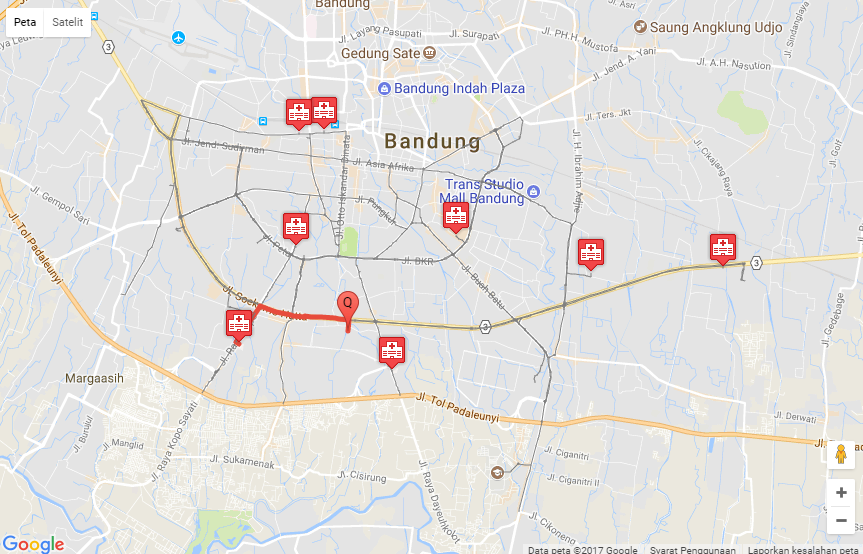
\includegraphics[scale=0.6]{rute_ambulans1.png}
    \caption{3-NN ambulance to emergency location}
    \label{fig:my_label}
\end{figure}

%
\chapter{Result and Discussion}
In this chapter will be described on the process of collecting and processing data and analysis results are performed in the methodology described in the previous discussion.

\section{Result of NVD Construction}
Determining nearest emergency unit required by dividing plane into each emergency unit coverage area. Every coverage area represent that the location inside it will returns its generator for nearest emergency unit. The NVD construction consists of several phases shown as below :

\subsubsection{Border Point Determination}
Conducted to obtain the outermost point of the power area of an emergency unit. Border point is done by tracing each path starting from the starting point of an emergency unit. Search continues until met to another emergency unit. Both units become neighbors separated by a border point that occupies the midpoint of the traced path.

The result of data processing to get border point is divided into 3 parts for each type of emergency unit. The second part is the determination of the border point for the police type unit that produces 44 border points and 16 neighborhoods. The second part is the determination of the border point for the emergency unit of ambulance which produces 29 border points and 10 neighborhoods. And the third part is the determination of the border point for the fire brigade unit that produces 19 border points and 4 neighborhoods. The result of determining the border point for each unit can be seen on figure \ref{fig:bp_pol}, \ref{fig:bp_amb}, and \ref{fig:bp_fbg}. While table \ref{table:adj_pol}, \ref{table:adj_amb}, and \ref{table:adj_fbg} shows neighbors between generators which share same border point.

\begin{figure}[H]
    \centering
    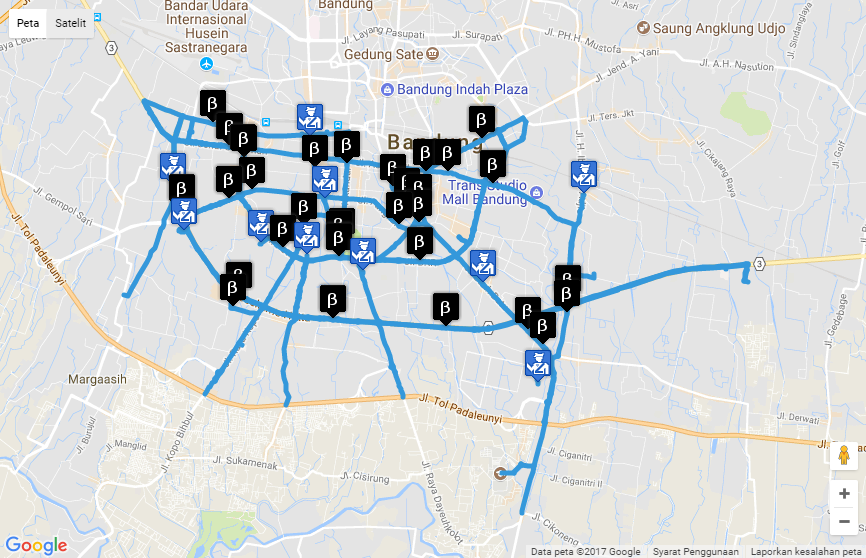
\includegraphics[scale=0.6]{v_border_point_pol.png}
    \caption{Border Point Determination Result for Police Unit}
    \label{fig:bp_pol}
\end{figure}

\begin{table}[H]
\centering
\begin{tabular}{|c|c|c|}
\hline
\textbf{No} & \textbf{Emergency Unit 1} & \textbf{Emergency Unit 2} \\ \hline
1           & Polsek Bandung Kidul      & Polsek Lengkong           \\ \hline
2           & Polsek Lengkong           & Polsek Regol              \\ \hline
3           & Polsek Lengkong           & Polsek Kiaracondong       \\ \hline
4           & Polsek Lengkong           & Polsek Astana Anyar       \\ \hline
5           & Polsek Lengkong           & Polsek Andir              \\ \hline
6           & Polsek Regol              & Polsek Bojongloa Kidul    \\ \hline
7           & Polsek Regol              & Polsek Astana Anyar       \\ \hline
8           & Polsek Andir              & Polsek Astana Anyar       \\ \hline
9           & Polsek Astana Anyar       & Polsek Bojongloa Kidul    \\ \hline
10          & Polsek Bojongloa Kaler    & Polsek Astana Anyar       \\ \hline
11          & Polsek Babakan Ciparay    & Polsek Bandung Kulon      \\ \hline
12          & Polsek Andir              & Polsek Bandung Kulon      \\ \hline
13          & Polsek Andir              & Polsek Bojongloa Kaler    \\ \hline
14          & Polsek Bojongloa Kidul    & Polsek Bojongloa Kaler    \\ \hline
15          & Polsek Bojongloa Kidul    & Polsek Babakan Ciparay    \\ \hline
16          & Polsek Bojongloa Kaler    & Polsek Babakan Ciparay    \\ \hline
\end{tabular}
\caption{Adjacency Generator Result for Police Unit}
\label{table:adj_pol}
\end{table}

\pagebreak



\begin{figure}[H]
    \centering
    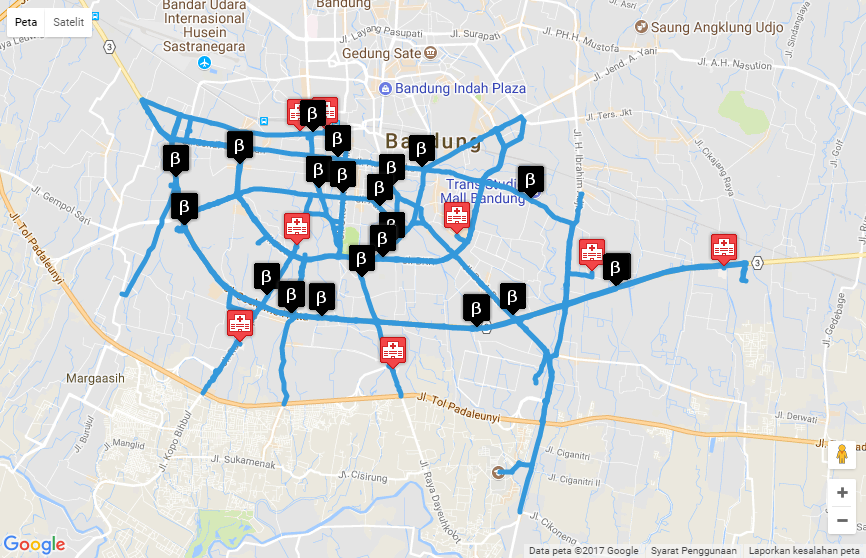
\includegraphics[scale=0.6]{v_border_point_amb.png}
    \caption{Border Point Determination Result for Ambulance Unit}
    \label{fig:bp_amb}
\end{figure}

\begin{table}[H]
\centering
\begin{tabular}{|c|c|c|}
\hline
\textbf{No} & \textbf{Emergency Unit 1} & \textbf{Emergency Unit 2} \\ \hline
1           & RSU Al-Islam              & RSU KCK Pindad            \\ \hline
2           & RSU Kebonjati             & RSU Santosa Central       \\ \hline
3           & RSU Immanuel              & RSU Kebonjati             \\ \hline
4           & RSU Immanuel              & RSU Santosa Central       \\ \hline
5           & RSU Muhammadiyah          & RSU Bandung Central       \\ \hline
6           & RSU Muhammadiyah          & RSU KCK Pindad            \\ \hline
7           & RSU Sartika Asih          & RSU KCK Pindad            \\ \hline
8           & RSU Immanuel              & RSU Sartika Asih          \\ \hline
9           & RSU Santosa Kopo          & RSU Immanuel              \\ \hline
10          & RSU Immanuel              & RSU Muhammadiyah          \\ \hline
\end{tabular}
\caption{Adjacency Generator Result for Ambulance Unit}
\label{table:adj_amb}
\end{table}

\pagebreak

\begin{figure}[H]
    \centering
    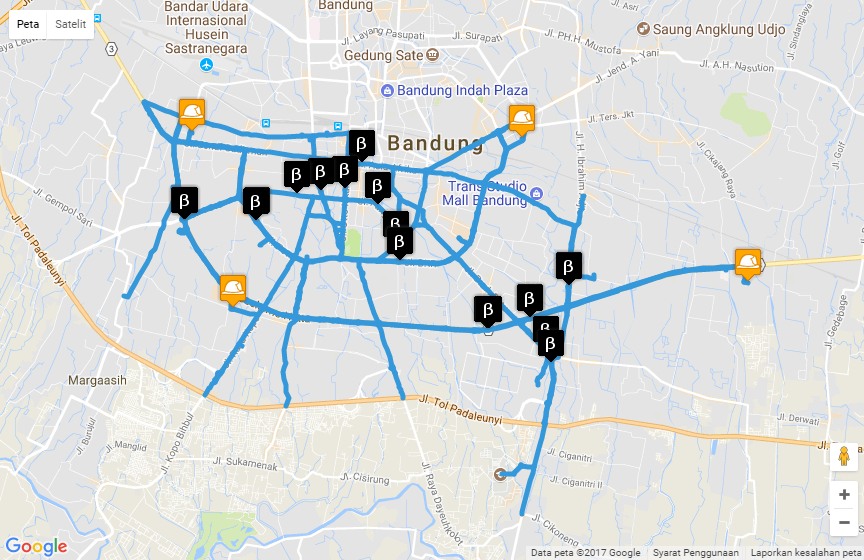
\includegraphics[scale=0.6]{v_border_point_fbg.png}
    \caption{Border Point Determination Result for Fire Brigade Unit}
    \label{fig:bp_fbg}
\end{figure}

\begin{table}[H]
\centering
\begin{tabular}{|c|c|c|}
\hline
\textbf{No} & \textbf{Emergency Unit 1} & \textbf{Emergency Unit 2} \\ \hline
1           & UPT Damkar Timur          & Dinas Kebakaran Bandung   \\ \hline
2           & UPT Damkar Barat          & Dinas Kebakaran Bandung   \\ \hline
3           & Dinas Kebakaran Bandung   & UPT Damkar Selatan        \\ \hline
4           & UPT Damkar Selatan        & UPT Damkar Barat          \\ \hline
\end{tabular}
\caption{Adjacency Generator Result for Fire Brigade Unit}
\label{table:adj_fbg}
\end{table}

\pagebreak
\subsubsection{Nearest Emergency Unit Classification}
The classification of the nearest emergency unit is used to classify the nearest unit for each location in Bandung so that each emergency unit has a coverage area indicating that the unit is the nearest unit. 

The results of the classification of the nearest emergency unit to obtain the coverage area of each unit is divided into 3 parts according to the type of emergency services. The first part is the nearest emergency unit classification for police which divides Bandung into 10 coverage area. The second part is the nearest emergency unit classification for ambulance that divides Bandung into 8 coverage area. The third part is the nearest emergency unit classification for fire brigade that divides Bandung into 4 coverage area. The results of NVD formation for each emergency unit can be shown on figure \ref{fig:nvd_pol}, \ref{fig:nvd_amb}, and \ref{fig:nvd_fbg}.

\begin{figure}[H]
    \centering
    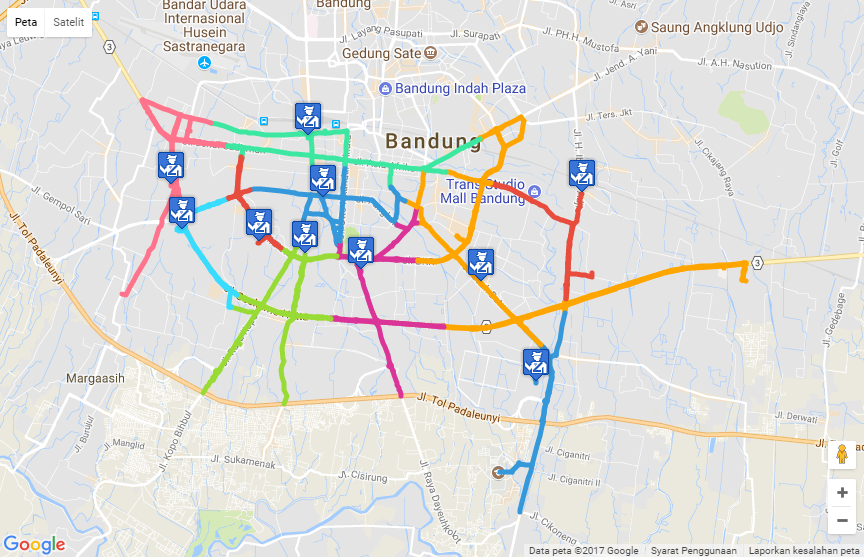
\includegraphics[scale=0.6]{v_nvd_pol.png}
    \caption{Network Voronoi Diagram for Police Unit}
    \label{fig:nvd_pol}
\end{figure}

\begin{figure}[H]
    \centering
    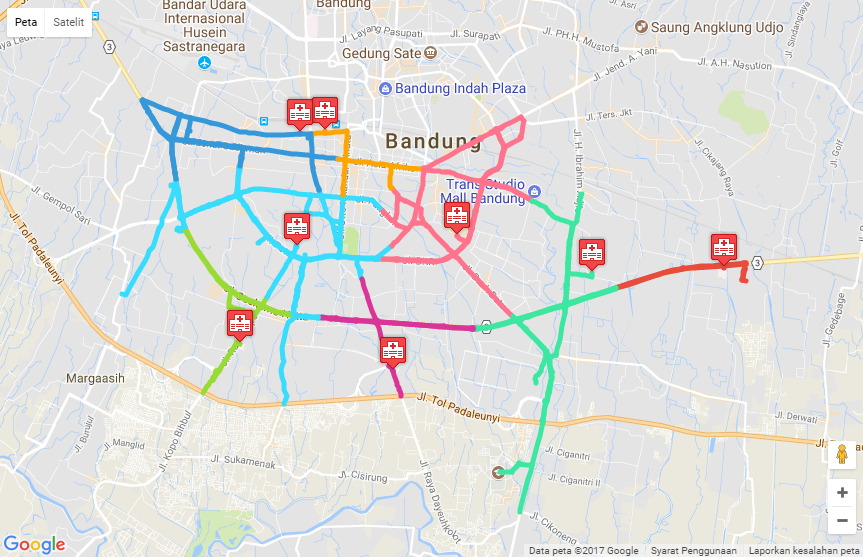
\includegraphics[scale=0.6]{v_nvd_amb.png}
    \caption{Network Voronoi Diagram for Ambulance Unit}
    \label{fig:nvd_amb}
\end{figure}

\begin{figure}[H]
    \centering
    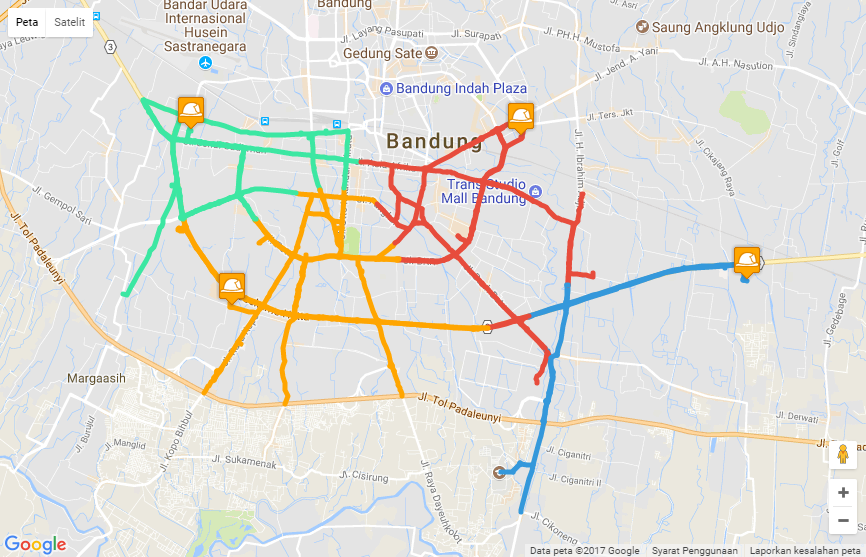
\includegraphics[scale=0.6]{v_nvd_fbg.png}
    \caption{Network Voronoi Diagram for Fire Brigade Unit}
    \label{fig:nvd_fbg}
\end{figure}

\pagebreak
\section{NVD-based KNN vs Basic KNN}
This experiment works by comparing overall performances of NVD-based KNN to basic KNN. The experiment used two real-world datasets. The first dataset consists a network of approximately 780 links and 500 nodes of the road system in Bandung. The second dataset consists of a set of points representing police, ambulance, and fire brigade in Bandung containing 10, 8 , and 4 objects, respectively. The experiment present the average results of 20 runs of k-nearest neighbor queries where k varied from 1 to 10.

\subsection{Accuracy}
The k-nearest emergency unit search accuracy test is divided into 2 parts using the NVD-based KNN and basic KNN algorithms. As shown in table \ref{table:accuracy_compare}, both algorithms returns 100\% of accuracy for finding k-nearest emergency unit. This means that both algorithm always get the right emergency units based on k-selected.

\begin{table}[H]
\centering
\resizebox{\textwidth}{!}{%
\begin{tabular}{|c|c|c|c|c|c|c|c|c|c|c|c|c|}
\hline
\multirow{3}{*}{\textbf{\begin{tabular}[c]{@{}c@{}}Emergency\\ Unit Type\end{tabular}}} & \multicolumn{12}{c|}{\textbf{Accuracy (\%)}}                                                                                                                                                                           \\ \cline{2-13} 
                                                                                        & \multicolumn{2}{c|}{\textbf{k=1}} & \multicolumn{2}{c|}{\textbf{k=2}} & \multicolumn{2}{c|}{\textbf{k=4}} & \multicolumn{2}{c|}{\textbf{k=6}} & \multicolumn{2}{c|}{\textbf{k=8}} & \multicolumn{2}{c|}{\textbf{k=10}} \\ \cline{2-13} 
                                                                                        & \textbf{NVD}    & \textbf{KNN}    & \textbf{NVD}    & \textbf{KNN}    & \textbf{NVD}    & \textbf{KNN}    & \textbf{NVD}    & \textbf{KNN}    & \textbf{NVD}    & \textbf{KNN}    & \textbf{NVD}     & \textbf{KNN}    \\ \hline
Police                                                                                  & 100             & 100             & 100             & 100             & 100             & 100             & 100             & 100             & 100             & 100             & 100              & 100             \\ \hline
Ambulance                                                                               & 100             & 100             & 100             & 100             & 100             & 100             & 100             & 100             & 100             & 100             & 100              & 100             \\ \hline
Fire Brigade                                                                            & 100             & 100             & 100             & 100             & 100             & 100             & 100             & 100             & 100             & 100             & 100              & 100             \\ \hline
\end{tabular}%
}
\caption{Accuracy Comparison between NVD-based KNN and basic KNN}
\label{table:accuracy_compare}
\end{table}

\begin{figure}[H]
    \centering
	\frame{    
    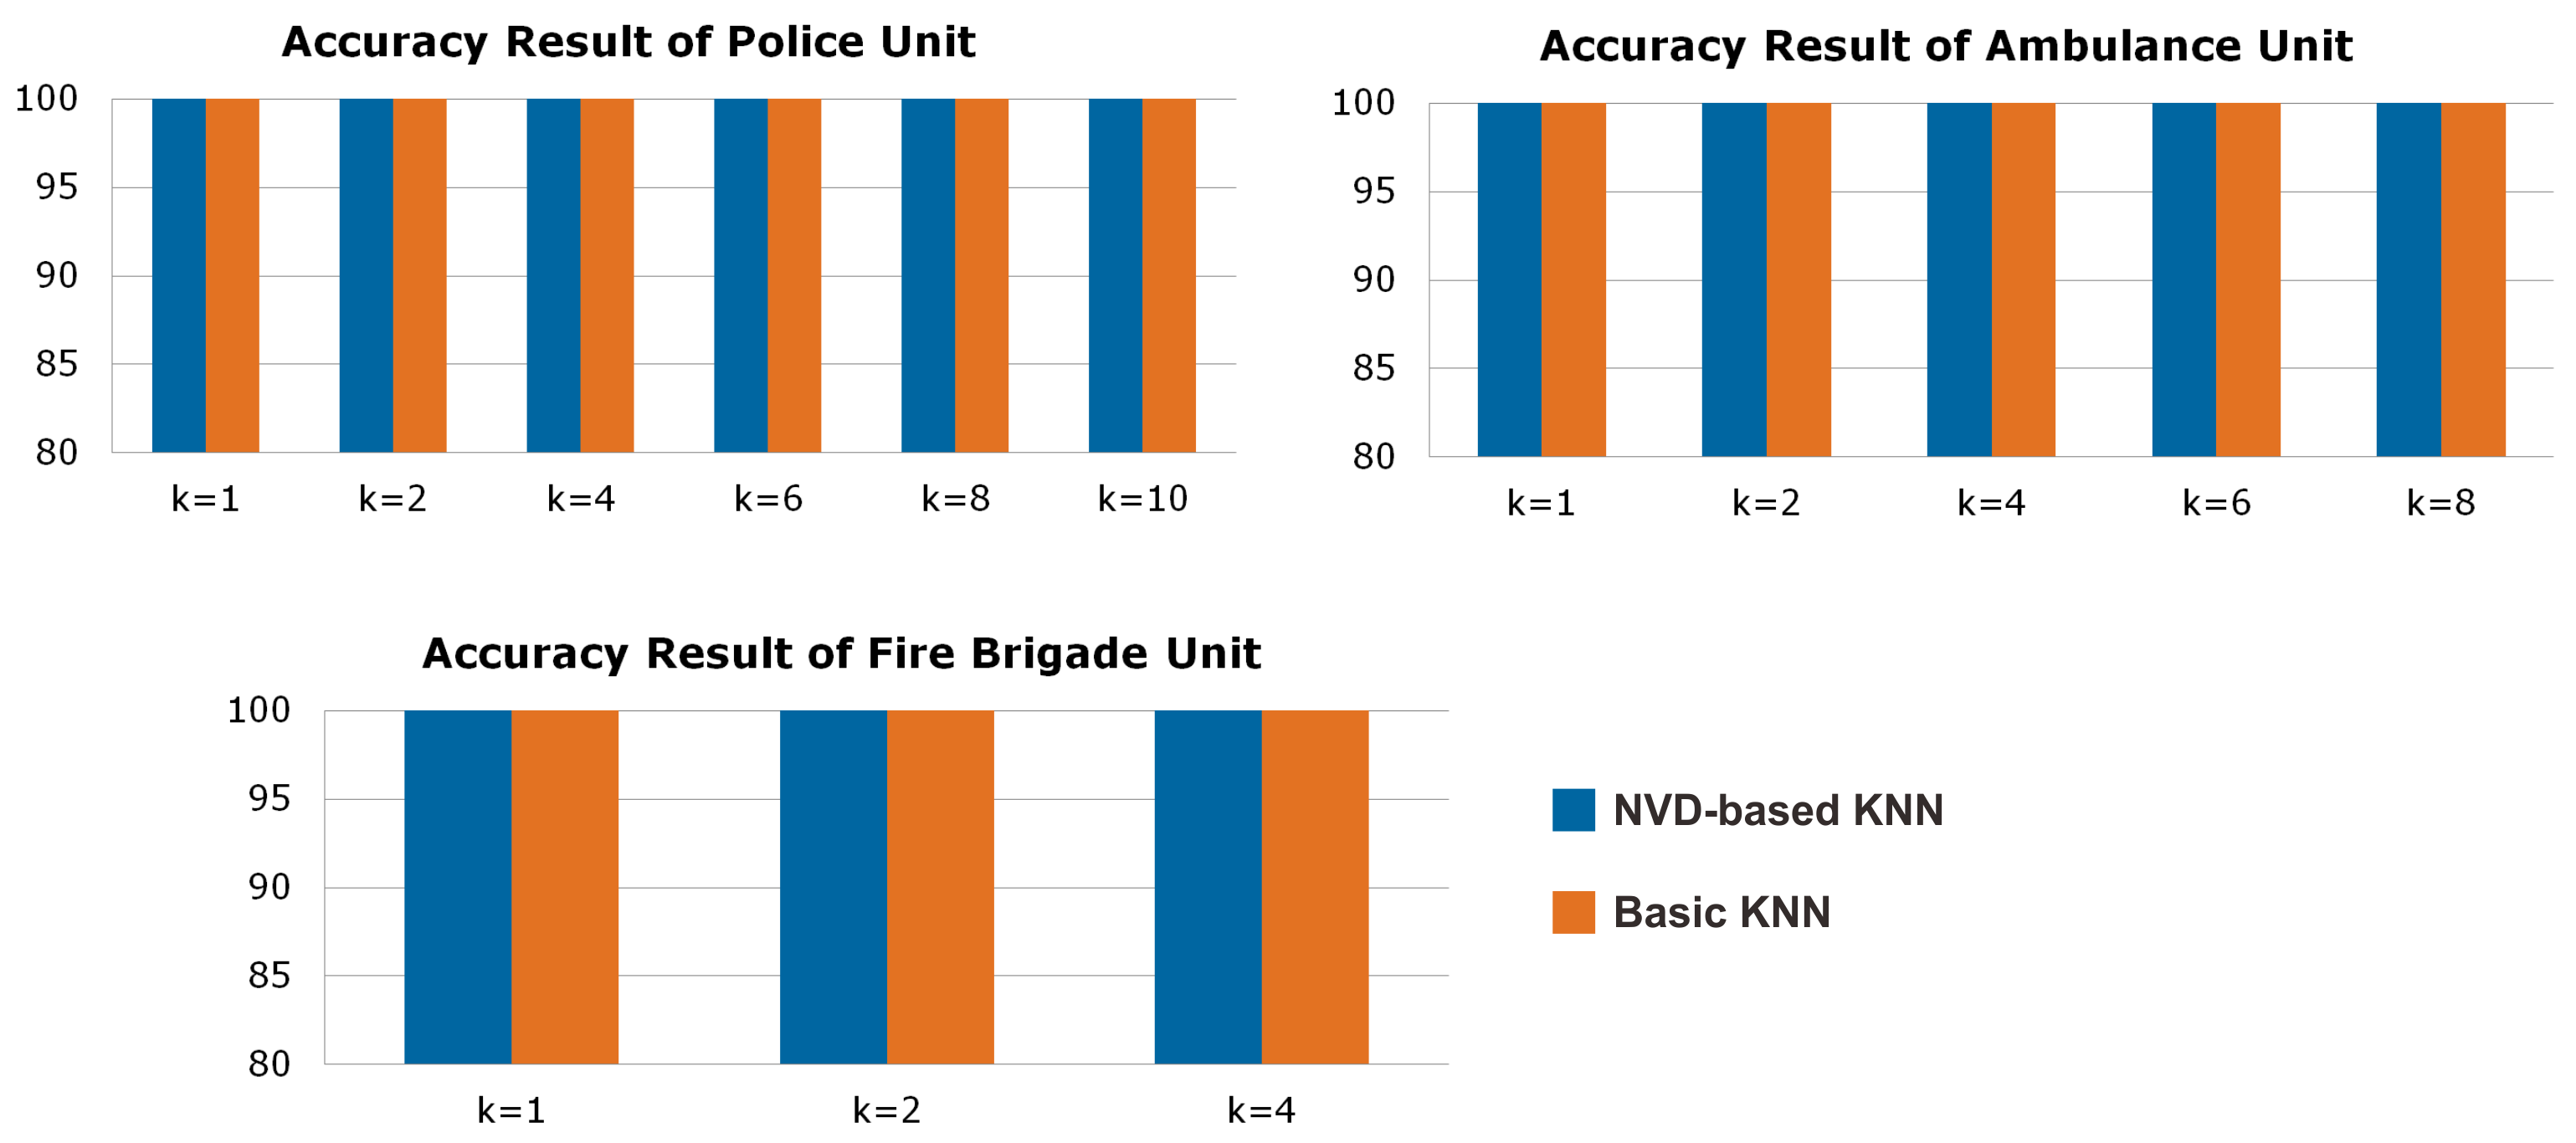
\includegraphics[scale=0.53]{v_accuracy.png}}
    \caption{Accuracy Comparison Chart \\ between NVD-based KNN and basic KNN}
    \label{fig:v_accuracy}
\end{figure}



\pagebreak
\subsection{Execution Time}
Experiment show that the total execution time of KNN based NVD less than that of KNN. Table \ref{table:execution_time_compare} shows the result of comparing total execution time between KNN based NVD and basic KNN. The first columns specify the emergency unit in Bandung. Note that for the given dataset, unit police and fire brigade represent the emergency units with the maximum and minimum number of units in Bandung. Basic KNN always returns stable execution time regardless k value. This because to find nearest emergency unit, KNN must measure all distance from emergency location to each emergency unit before sorting it based on minimum distance. So when k=1 NVD-based KNN generates the result set almost instantly. This is because NVD has generate territory for each emergency unit so its enough to find 1-NN by only looking for which unit emergency location exists. However, basic KNN requires between 0.25 to 0.57 seconds to provide 1-NN. For larger k, NVD-based KNN has a total execution time similarly with basic KNN. This is because each unit has been candidates and measured its  distance to emergency location.

\begin{table}[H]
\centering
\resizebox{\textwidth}{!}{%
\begin{tabular}{|c|c|c|c|c|c|c|c|c|c|c|c|c|}
\hline
\multirow{3}{*}{\textbf{\begin{tabular}[c]{@{}c@{}}Emergency\\ Unit Type\\ (density)\end{tabular}}} & \multicolumn{12}{c|}{\textbf{Execution Time (s)}}                                                                                                                                                                      \\ \cline{2-13} 
                                                                                                    & \multicolumn{2}{c|}{\textbf{k=1}} & \multicolumn{2}{c|}{\textbf{k=2}} & \multicolumn{2}{c|}{\textbf{k=4}} & \multicolumn{2}{c|}{\textbf{k=6}} & \multicolumn{2}{c|}{\textbf{k=8}} & \multicolumn{2}{c|}{\textbf{k=10}} \\ \cline{2-13} 
                                                                                                    & \textbf{KNN}    & \textbf{NVD}    & \textbf{KNN}    & \textbf{NVD}    & \textbf{KNN}    & \textbf{NVD}    & \textbf{KNN}    & \textbf{NVD}    & \textbf{KNN}    & \textbf{NVD}    & \textbf{KNN}     & \textbf{NVD}    \\ \hline
\begin{tabular}[c]{@{}c@{}}Police\\ (0.0127)\end{tabular}                                           & 0.57            & 0.04            & 0.57            & 0.17            & 0.57            & 0.34            & 0.57            & 0.41            & 0.57            & 0.53            & 0.57             & 0.54            \\ \hline
\begin{tabular}[c]{@{}c@{}}Ambulance\\ (0.0102)\end{tabular}                                        & 0.47            & 0.04            & 0.47            & 0.11            & 0.47            & 0.34            & 0.47            & 0.39            & 0.47            & 0.42            & -                & -               \\ \hline
\begin{tabular}[c]{@{}c@{}}Fire Brigade\\ (0.0051)\end{tabular}                                     & 0.25            & 0.05            & 0.25            & 0.14            & 0.25            & 0.2             & -               & -               & -               & -               & -                & -               \\ \hline
\end{tabular}%
}
\caption{Execution Time Comparison \\ between NVD-based KNN and basic KNN}
\label{table:execution_time_compare}
\end{table}


\begin{figure}[H]
    \centering
	\frame{    
    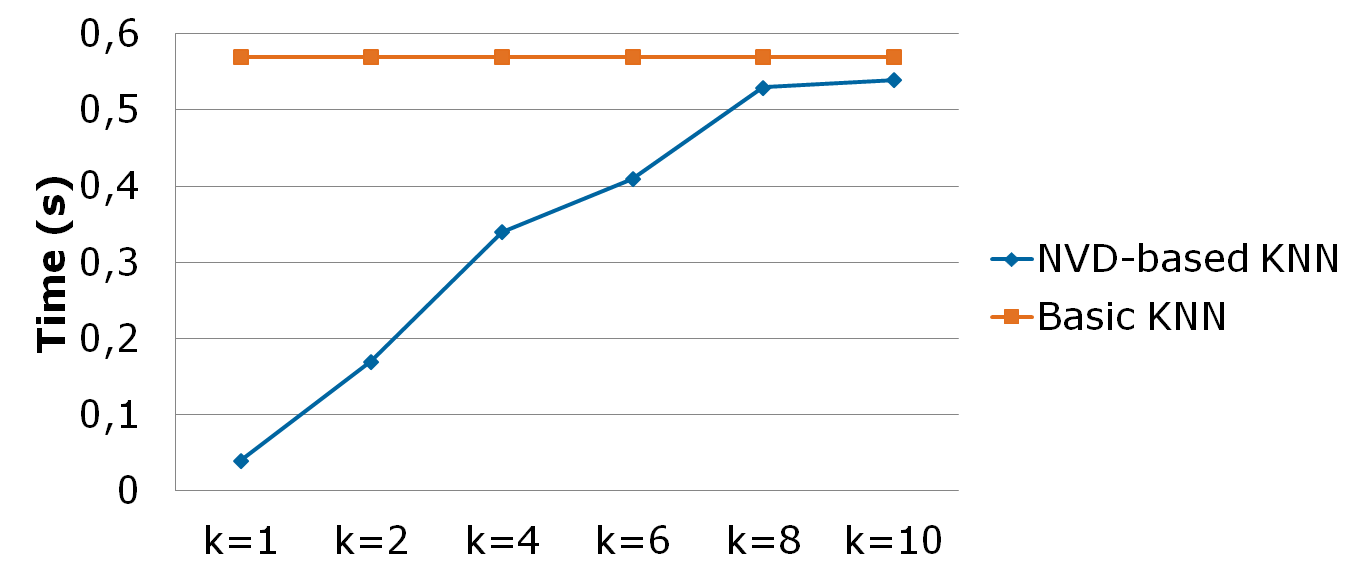
\includegraphics[scale=0.5]{execution_time_comparison_pol.png}}
    \caption{Execution Time Comparison Graph for Police Unit}
    \label{fig:v_bp_ambulance}
\end{figure}

\begin{figure}[H]
    \centering
	\frame{    
    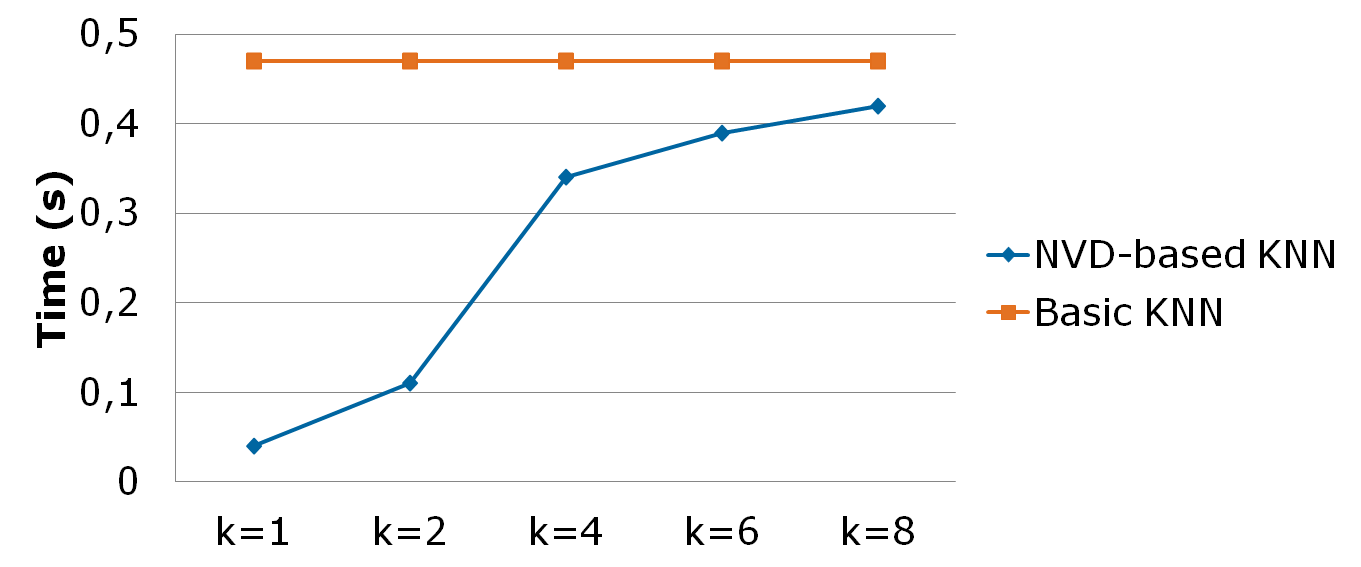
\includegraphics[scale=0.5]{execution_time_comparison_amb.png}}
    \caption{Execution Time Comparison Graph for Ambulance Unit}
    \label{fig:v_bp_ambulance}
\end{figure}

\begin{figure}[H]
    \centering
	\frame{    
    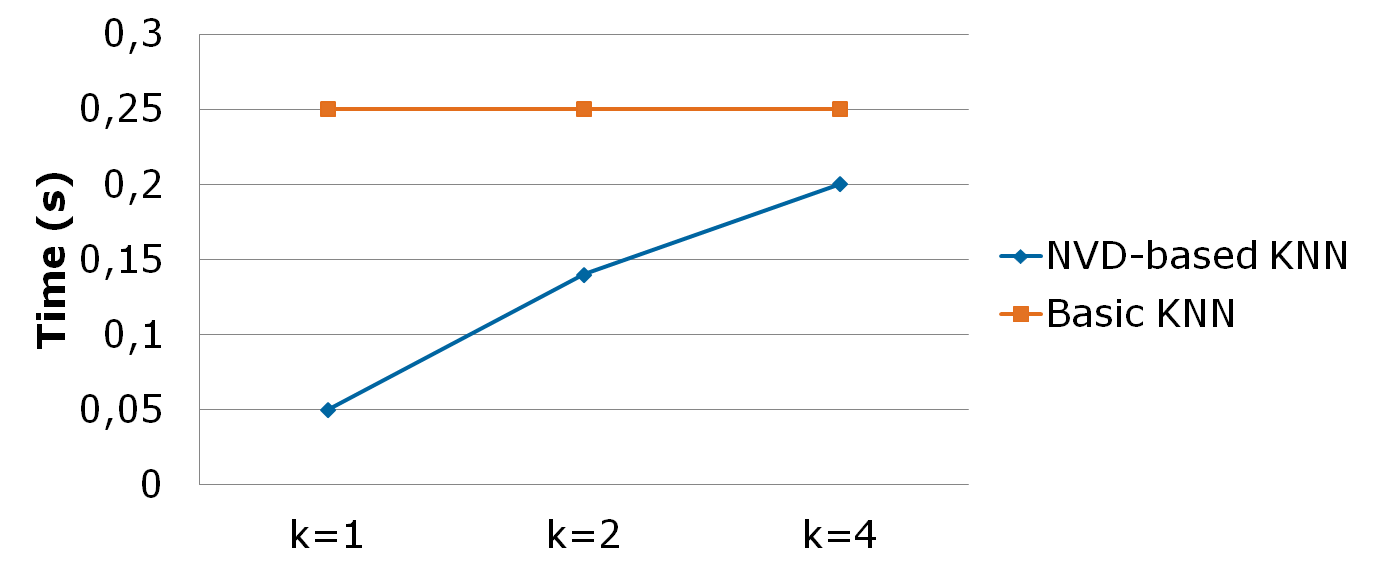
\includegraphics[scale=0.5]{execution_time_comparison_fbg.png}}
    \caption{Execution Time Comparison Graph for Fire Brigade Unit}
    \label{fig:v_bp_ambulance}
\end{figure}


%
\chapter{Conclusion and Suggestion}
This chapter describes conclusions of this final project that has been done and also suggestions which contain the things that should be considered for further development. The conclusions and suggestions are described in detail in the following sub-chapters:
\section{Conclusion}
Based on the results of this final project that has been done, can be drawn conclusions that refers to the objectives into the following subsection:
\begin{enumerate}
\item All objectives are successfully designed implemented using NVD-based KNN approach

\item NVD-based KNN and basic KNN has 100\% accuracy levels which means both algorithms always return correct k-nearest emergency units.

\item NVD-based KNN outperforms basic KNN in execution time by a factor of 1.05 to 14.25 depending on the value of k for determining nearest emergency units.
\end{enumerate}

\section{Suggestion}
Suggestions that can be submitted from the results of this study for further research development are as follows:
\begin{enumerate}
\item Adding another emergency services.
\item Finding k-nearest emergency unit based on travel time by considering road conditions.
\end{enumerate}

%
\cleardoublepage
\addcontentsline{toc}{chapter}{References}
\bibliographystyle{acm} %harvard style
\bibliography{References}
%
%\pagebreak
\end{document}
